\documentclass{book}

% Packages
\usepackage{amsmath}
\usepackage{array}
\usepackage{enumitem}
\usepackage{float}
\usepackage[T1]{fontenc}
\usepackage{geometry}
\usepackage{graphicx}
\usepackage[colorlinks=true,linkcolor=blue,urlcolor=blue,citecolor=blue]{hyperref}     
\usepackage[utf8]{inputenc}
\usepackage{listings}
\usepackage{tabularx}
\usepackage{tcolorbox}
\usepackage{tikz}
\usepackage{xcolor}
\usepackage[table]{xcolor}
\usepackage{verbatim}


% Define colors
\definecolor{grayheavy}{gray}{0.7}
\definecolor{graylight}{gray}{0.8}
\definecolor{graysuperlight}{gray}{0.9}

\usetikzlibrary{shapes.geometric}
\usetikzlibrary{positioning}  

% Page layout
\geometry{margin=1in}

\tikzstyle{startstop} = [rectangle, rounded corners, minimum width=3cm, minimum height=1cm,text centered, draw=black, fill=red!30]
\tikzstyle{process} = [rectangle, minimum width=3cm, minimum height=1cm, text centered, draw=black, fill=blue!30]
\tikzstyle{condition} = [diamond, minimum width=3cm, minimum height=1cm, text centered, draw=black, fill=white!100]
\tikzstyle{file} = [rectangle, minimum width=3cm, minimum height=1cm, text centered, draw=black, fill=gray!30]
\tikzstyle{arrow} = [thick,->,>=stealth]  
\tikzstyle{line} = [thick,-,>=stealth]  

% Functions
\tcbset{
    attentionbox/.style={
        colback=red!5, % Background color
        colframe=red!75!black, % Border color
        coltitle=black, % Title color
        boxrule=0.8mm, % Thickness of the border
        left=2mm, % Left padding
        before skip=5mm, % Space before the box
        after skip=5mm, % Space after the box
        sharp corners, % Sharp corners for the box
        fonttitle=\bfseries, % Bold title font
        attach boxed title to top left={yshift=-2mm,xshift=2mm}, % Title position
        boxed title style={
            size=small,
            colback=red!50,
            colframe=red!75!black,
            sharp corners,
        },
    }
}

% % Code formatting
\lstset{
    language=Python,
    basicstyle=\ttfamily\fontsize{9}{10}\selectfont,
    breaklines=true,
    frame=single,
    keywordstyle=\color{blue},
    commentstyle=\color{green!70!black},
    stringstyle=\color{red},
    showstringspaces=false,
    numbers=left,
    numberstyle=\tiny\color{gray},
    stepnumber=1,
    numbersep=10pt,
    xleftmargin=5mm,
}

\newcommand{\mypart}[1]{\setcounter{chapter}{0} \part{#1}}
\renewcommand{\theHsection}{\thepart.section.\thesection}

\title{The HDF5\_BLS package and its user interface}
\author{Pierre Bouvet}
\date{\today}

\begin{document}

\maketitle

\tableofcontents

\chapter*{Introduction}\addcontentsline{toc}{chapter}{Introduction}
    Welcome to the interactive UI tutorial. This book will guide you through the steps to create and use the UI effectively.

The HDF5\_BLS package is a Python library for handling Brillouin light scattering (BLS) data and converting it into a standardized HDF5 format. The library provides functions to open raw data files, store their properties, convert them into a Power Spectral Density (PSD) and analyze the PSD with a standardized treatment protocol. The library is currently compatible with the following file formats:
\begin{itemize}
    \item \textbf{*.dat} files: spectra returned by the GHOST software or obtained using Time Domain measurements
    \item \textbf{*.tif} files: an image format that can be used to export 2D detector images.
    \item \textbf{*.npy} files: an arbitrary numpy array
    \item \textbf{*.sif} files: image files obtained with Andor cameras
\end{itemize}

The package comes with a graphical user interface (GUI) that allows users to easily open, edit, and save data. This interface is the preferred way to use the package and the subject of this tutorial. The GUI is currently compatible with the following spectrometers:
\begin{itemize}
    \item Tandem Fabry-Perot (TFP) spectrometers
    \item Angle-resolved VIPA (ar-VIPA) spectrometers 
\end{itemize}

    
\chapter*{Preamble: The project in a nutshell}\addcontentsline{toc}{chapter}{Preamble: The project in a nutshell}
    \section*{HDF5 file structure}\addcontentsline{toc}{section}{HDF5 file structure}
        \subsection*{Basic file structure}\addcontentsline{toc}{subsection}{Basic file structure}
            The vision of the project is to unify all BLS data into a single HDF5 file. This file will be used to store all the data and metadata of the BLS. The data will be stored in a hierarchical structure, all the data related to BLS being stored the "Data" group. This choice allows results from other techinques to be stored in the same file, only in other, independent groups, to minimize the risk of nomenclature competition between techinques. The "Data" group will contain all the data. These data are arranged in groups, whose identifiers are "Data\_i". Each group can only contain one measure, in the form of an array, whose dimension is however not restricted. This measure will be called "Raw\_data". The attributes of the measure are stored in the group attributes.

The following structure represents the base structure of the file:

\begin{verbatim}
    file.h5
    +-- Data (group)
    |   +-- Data_1 (group)
    |   |   +-- Raw_data (dataset)
\end{verbatim}

        
        \subsection*{Meta-files}\addcontentsline{toc}{subsection}{Meta-files}
            The Hierarchical Data Format (HDF5) finds its interest in storage for our community, of different measures. These result in "meta-files" where data corresponding to different experiments can be found. The organization of such a file will follow a structure similar to this one:

\begin{verbatim}
    file.h5
    +-- Brillouin (group)
    |   +-- RWPE1 organoids (group)
    |   |   +-- Morphogenesis day 1 (group)
    |   |   |   +-- Sample 1 (group)
    |   |   |   |   +-- Measure (dataset)
    |   |   |   +-- Sample 2 (group)
    |   |   |   +-- ...
    |   |   +-- Morphogenesis day 2 (group)
    |   |   +-- ...
    |   +-- H6C7 organoids
    |   ...
\end{verbatim}

Although no rules are imposed on the way to organize the file, we propose to associate a hierarchical level to an hyperparameter that has been varied for the experiment. In the given example:
\begin{itemize}
    \item The first hierarchical level is associated to the cell line that is observed
    \item The second hierarchical level is associated to the day of the experiment
    \item The third hierarchical level is associated to the sample that was measured
\end{itemize}

Note that the format does not impose any restriction on the names of the groups nor the measures. This choice allows you to create user-friendly files that can be opened with any software that can read HDF5 files (e.g. HDFView, HDFCompass, Fiji, H5Web, etc.).
        
        \subsection*{Attributes}\addcontentsline{toc}{subsection}{Attributes}
            \subsubsection*{Storing the attributes of the data in its metadata}

    HDF5 file format allows the storage of attributes in the metadata of the groups and datasets. We therefore propose to store all the attributes concerning an experiment in the metadata of its parent group:
    \begin{verbatim}
        file.h5
        +-- Brillouin (group)
        |   +-- Measure (group) -> attributes of the measure
        |   |   +-- Measure (dataset) 
    \end{verbatim}

    Being a hierarchical format, we also propose to store attributes hierarchically: all attributes of parent group apply to childre groups (if not redefined in children groups). Storing attributes in large files can therefore be done the following way:
    \begin{verbatim}
        file.h5
        +-- Brillouin (group) -> attributes shared by Measure 0 and Measure 1
        |   +-- Measure 0 (group) -> other attributes specific to Measure 0
        |   |   +-- Measure (dataset)
        |   +-- Measure 1 (group) -> other attributes specific to Measure 1
        |   |   +-- Measure (dataset)
    \end{verbatim}

    Note that the access to the whole list of attributes applying to a group or dataset will be possible with the HDF5\_BLS package (see \hyperref[subchapter:wrapper.get_attributes]{Wrapper.get\_attributes}).

\subsubsection*{Types of attributes}

    In an effort to avoid any incompatibility, we propose to store the values of the attributes as ascii-encoded text. The library will then convert the strings to the appropriate type (e.g. float, int, etc.).

\subsubsection*{Organization of the attributes}

    \paragraph*{Prefix}
    We differentiate 5 types of attributes, that we differentiate using the following prefixes:
    \begin{itemize}
        \item \textbf{SPECTROMETER} - Attributes that are specific to the spectrometer used, such as the wavelength of the laser, the type of laser, the type of detector, etc. These attributes are recognized by the capital letter word "SPECTROMETER" in the name of the attribute.
        \item \textbf{MEASURE} - Attributes that are specific to the sample, such as the date of the measure, the name of the sample, etc. These attributes are recognized by the capital letter word "MEASURE" in the name of the attribute.
        \item \textbf{FILEPROP} - Attributes that are specific to the original file format, such as the name of the file, the date of the file, the version of the file, the precision used on the storage of the data, etc. These attributes are recognized by the capital letter word "FILEPROP" in the name of the attribute.
        \item \textbf{PROCESS} - Attributes that are specific to the storage of algorithms. These attributes are recognized by the capital letter word "PROCESS" in the name of the attribute.
        \item Attributes that are used inside the HDF5 file, such as the "Brillouin\_type" attribute. These attributes are the only ones without a prefix.
    \end{itemize}

    \paragraph*{Units}
    The name of the attributes contains the unit of the attribute if it has units, in the shape of an underscore followed by the unit in parenthesis. Some parameters will also be given following a given norm, such as the ISO8601 for dates. These norms are not specified in the name of the attribute. Here are some examples of attributes:
    \begin{itemize}
        \item "SPECTROMETER.Detector\_Type" is the type of the detector used.
        \item "MEASURE.Sample" is the name of the sample.
        \item "MEASURE.Exposure\_(s)" is the exposure of the sample given in seconds
        \item "MEASURE.Date\_of\_measurement" is the date of the measurement, stored following the ISO8601 norm.
        \item "FILEPROP.Name" is the name of the file.
    \end{itemize}

\subsubsection*{Unifification and Versioning of attributes}
    To unify the name of attributes between laboratories, we propose to use a spreadsheet that contains the list of attributes, their definition, their unit and an example of value. This spreadsheet is available on the project repository and is updated as new attributes are added to the project. Each attribute has a version number that is also stored in the attributes of each data attribute (under FILEPROP.version).

    This spreadsheet will also be the preferred way to define attributes for the measures and the HDF5\_BLS package allows to read and import the attributes directly from this spreadsheet (see \hyperref[subchapter:wrapper.import_properties_data]{Wrapper.import\_properties\_data}).
    
\subsubsection*{Storing analysis and treatment processes}

    Analysis and treatment processes are stored in the "PROCESS" attribute of the treatment groups. This attribute is a JSON file converted to a string, which contains the list of treatment steps performed on the data. This JSON file has the following structure:
    \begin{verbatim}
{
    "name": "The name of the algorithm",
    "version": "v 0.1",
    "author": "Author name and affiliation",
    "description": "The description of the algorithm",
    "functions": [
    {
        "function": "The 1st function name in the class",
        "parameters": {
            "parameter_1": value,
            "parameter_2": value,
            ...
        },
        "description": "The description of the function"
    },
    {
        "function": "The 2nd function name in the class",
        "parameters": {
            "parameter_1": value,
            "parameter_2": value,
            ...
        },
        "description": "The description of the function"
    },
    ...
    ]
}
    \end{verbatim}

    When the treatment is performed using the modules of the HDF5\_BLS package, this attribute is automatically updated. Note that custom treatments can also be stored in this attribute by the user.

    This attribute can be exported to a standalone JSON file using the library. This attribute also allows the library to re-apply the treatment to the data, and modify steps of the treatment if needed.
    
        
        \subsection*{The BLS\_type attribute}\addcontentsline{toc}{subsection}{The BLS\_type attribute}\label{subsec:preamble.file_structure.complete_structure}
            To improve user-friendliness of the format for the BioBrillouin community, we propose to add a new attribute: \textit{BLS\_type} to the groups and datasets of the file. This attribute will allow the user to quickly differentiate the content of the groups and datasets, and will also allow the automation of certain tasks.

For groups, this attribute can have the following values:
\begin{itemize}
    \item "Calibration\_spectrum": the group contains a calibration spectrum.
    \item "Impulse\_response": the group contains an impulse response function.
    \item "Measure": the group contains a measure (value by default).
    \item "Root": used to specify that the group is a structure group that contains other groups.
    \item "Treatment": the group contains treated data derived from a PSD and frequency arrays located in its parent group.
\end{itemize}

For datasets, this attribute can have the following values:
\begin{itemize}
    \item "Abscissa\_...": An abscissa array for the measures where the dimensions on which the dataset applies are given after the underscore.
    \item "Amplitude": The dataset contains the values of the fitted amplitudes.
    \item "Amplitude\_err": The dataset contains the error of the fitted amplitudes.
    \item "BLT": The dataset contains the values of the fitted amplitudes.
    \item "BLT\_err": The dataset contains the error of the fitted amplitudes.
    \item "Frequency": A frequency array associated to the power spectral density
    \item "Linewidth": The dataset contains the values of the fitted linewidths.
    \item "Linewidth\_err": The dataset contains the error of the fitted linewidths. 
    \item "PSD": A power spectral density array
    \item "Raw\_data": The dataset containing the raw data obtained after a BLS experiment.
    \item "Shift": The dataset contains the values of the fitted frequency shifts.
    \item "Shift\_err": The dataset contains the error of the fitted frequency shifts.
    \item "Other": The dataset contains other data that will not be used by the library.
\end{itemize}


\paragraph*{Example of an abscissa dataset:}
Let's consider a dataset consisting of 10x10 point mappings of cells in a grid of $10\mu m$ by $10\mu m$. We can store the abscissa in two ways:
\begin{itemize}
    \item We can store the abscissa as two 1D array of 10 elements each, for axis x and y for example. The array corresponding to the x axis will be stored in the dataset with the attribute "Brillouin\_type" set to "Abscissa\_0\_1". The array corresponding to the y axis will be stored in the dataset with the attribute "Brillouin\_type" set to "Abscissa\_1\_2".
    \item We can store the abscissa as a 2D array of 10x10 elements. This array will be stored in the dataset with the attribute "Brillouin\_type" set to "Abscissa\_0\_2".
\end{itemize}
A dedicated function is meant to do this step without the user having to worry about the attribute names. 

% Examples of HDF5 files with mappings can be found in the repository under the "guides/Tutorial/examples" folder.

\textbf{Note:} The "Brillouin\_type" attribute is not mandatory, but it is highly recommended to use it to differentiate the content of the groups and datasets. If this parameter is not present, the library will assume that group are "Root" group if they contain other groups and a "Measure" dataset if not, and that datasets are "Other" datasets.
        
        \subsection*{A base example}\addcontentsline{toc}{subsection}{A base example}\label{subsec:preamble.file_structure.some_examples}
            A single measure that has been treated, together with a calibration spectrum and an impulse response (both stored as a couple of Power Spectra Density and Frequency), will be stored in the following structure (the "Brillouin\_type" attribute is indicated in slanted text):

\noindent file.h5\\
+ Brillouin (group, \textit{Root})\\
|\indent + IRF (group, \textit{Impulse\_response})\\
|\indent |\indent + PSD (dataset, \textit{PSD})\\
|\indent |\indent + Frequency (dataset, \textit{Frequency})\\
|\indent + Calibration Water (group, \textit{Calibration\_spectrum})\\
|\indent |\indent + PSD (dataset, \textit{PSD})\\
|\indent |\indent + Frequency (dataset, \textit{Frequency})\\
|\indent + Measure (group, \textit{Measure})\\
|\indent |\indent + Raw measure (dataset, \textit{Raw\_data})\\
|\indent |\indent + PSD (dataset, \textit{PSD})\\
|\indent |\indent + Frequency (dataset, \textit{Frequency})\\
|\indent |\indent + Treatment (dataset, \textit{Treatment})\\
|\indent |\indent |\indent + Shift (dataset, \textit{Shift})\\
|\indent |\indent |\indent + Linewidth (dataset, \textit{Linewidth})\\
|\indent |\indent |\indent + Shift error (dataset, \textit{Shift\_err})\\
|\indent |\indent |\indent + Linewidth error (dataset, \textit{Linewidth\_err})\\


Note: The name of the groups and datasets are left to the user, note that the Brillouin\_type attribute allows to unambiguously differentiate each group and dataset.

Other examples can be found in \hyperref[chap:examples_file_structures]{appendix}


    \section*{A unified way to go from Measure to Results}\addcontentsline{toc}{section}{A unified way to go from Measure to Results}
        This format is designed to unify the way to store data in the BioBrillouin Community. From there, we propose to unify the treatment and analysis of the data. The storage being independent from the analysis, we propose to create an intermediate step where a Power Spectral Density is obtained.

The treatment of any PSD being essentially the same: a fitting of one or several lineshapes that takes into account the response of the instrument to deconvolve its effect, we further propose to unify the analysis after obtaining the PSD. This results in the following pipeline for any BLS experiment

\begin{figure}[H]
    \centering
    \small
    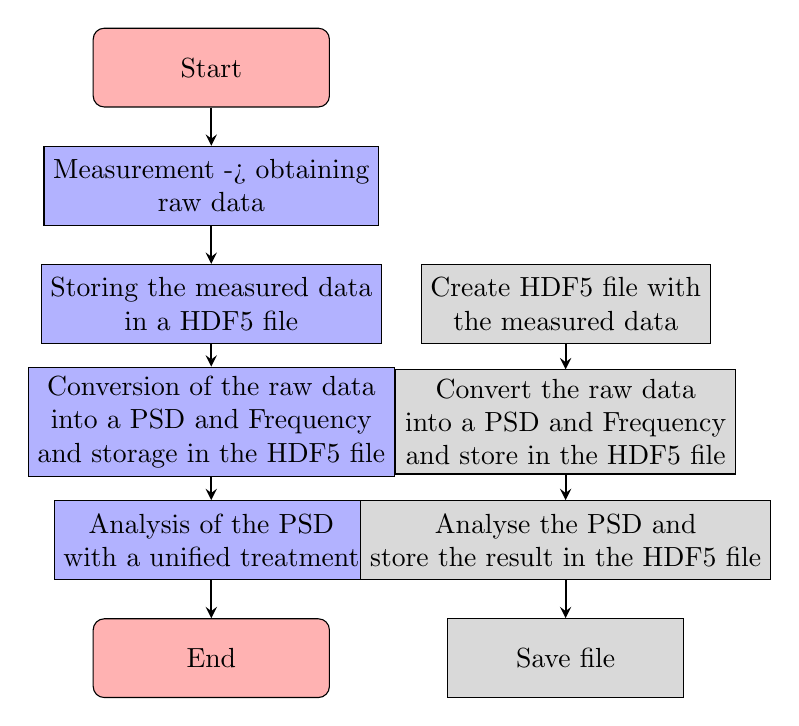
\begin{tikzpicture}[node distance=1.5cm]
        \node (start) [startstop] {Start};
        \node (acquire) [process, below of=start, align=center] {Measurement -> obtaining\\ raw data};
        \node (storage) [process, below of=acquire, align=center] {Storing the measured data\\ in a HDF5 file};
        \node (psd) [process, below of=storage, align=center] {Conversion of the raw data\\ into a PSD and Frequency\\ and storage in the HDF5 file};
        \node (fits) [process, below of=psd, align=center] {Analysis of the PSD\\ with a unified treatment};
        \node (end) [startstop, below of=fits] {End};

        \draw [arrow] (start) -- (acquire);
        \draw [arrow] (acquire) -- (storage);
        \draw [arrow] (storage) -- (psd);
        \draw [arrow] (psd) -- (fits);
        \draw [arrow] (fits) -- (end);

        \node (filestart) [file, right of=storage, xshift=3cm, align=center] {Create HDF5 file with\\ the measured data};
        \node (fileraw) [file, below of=filestart, align=center] {Convert the raw data\\ into a PSD and Frequency\\ and store in the HDF5 file};  
        \node (filetreat) [file, below of=fileraw, align=center] {Analyse the PSD and\\ store the result in the HDF5 file};
        \node (fileend) [file, below of=filetreat] {Save file};

        \draw [arrow] (filestart) -- (fileraw);
        \draw [arrow] (fileraw) -- (filetreat);
        \draw [arrow] (filetreat) -- (fileend);
    \end{tikzpicture}
    \caption{Flowchart of the pipeline}
\end{figure}




\mypart{HDF5\_BLS package tutorial}\label{chapter:tutorial}
    \chapter*{Installation and presentation}\addcontentsline{toc}{chapter}{Installation and presentation}
        \section{Installation}
    To get started, you need to install the repository. Follow the instructions below:

\begin{itemize}
    \item Step 1: Make sure you have Python 3.10 or higher installed. You can download Python at \href{https://www.python.org/downloads/}{this link}.
    \item Step 2: Clone the repository at \href{https://github.com/bio-brillouin/HDF5_BLS/tree/main}{this link}.    
    \item Step 3: Create a virtual environment and install the requirements. To do so, open a terminal, navigate to the repository folder and install the requirements. For windows users, you can open the terminal into the cloned and extracted repository (shift+left click over the folder -> Open in terminal) and use the following command:
\begin{lstlisting}
python -m venv venv
.\venv\Scripts\activate
pip install -r requirements_GUI.txt
\end{lstlisting}
    For Mac users, you can navigate to the repository, make sure you can view the path bar at the bottom of Finder (if not, check View/Show Path Bar in the menu bar), then press control and left click on the folder and select "Open in Terminal". Then, use the following command:
\begin{lstlisting}
python -m venv venv
source venv/bin/activate
pip install -r requirements_GUI.txt
\end{lstlisting}
    For Linux users, you can navigate to the repository, open a terminal in the folder and use the same command as for Mac users.
    \item Step 4: Run the \texttt{HDF5\_BLS\_GUI/main.py} file with
\begin{lstlisting}
python HDF5\_BLS\_GUI/main.py
\end{lstlisting}
\end{itemize}

\section{Presentation}
    The HDF5\_BLS\_GUI is a graphical user interface for the HDF5\_BLS package, designed to facilitate the exploration and analysis of HDF5 files. It provides a user-friendly environment for users to interact with their data, visualize results, and manage their workflows.

The GUI is built using the PySide6 library, which is a Python binding for the Qt framework. This library allows the GUI to be developed using a similar syntax to traditional Python code, making it easier to understand and maintain.

The GUI opens to the following window:
\begin{figure}[H]
    \centering
    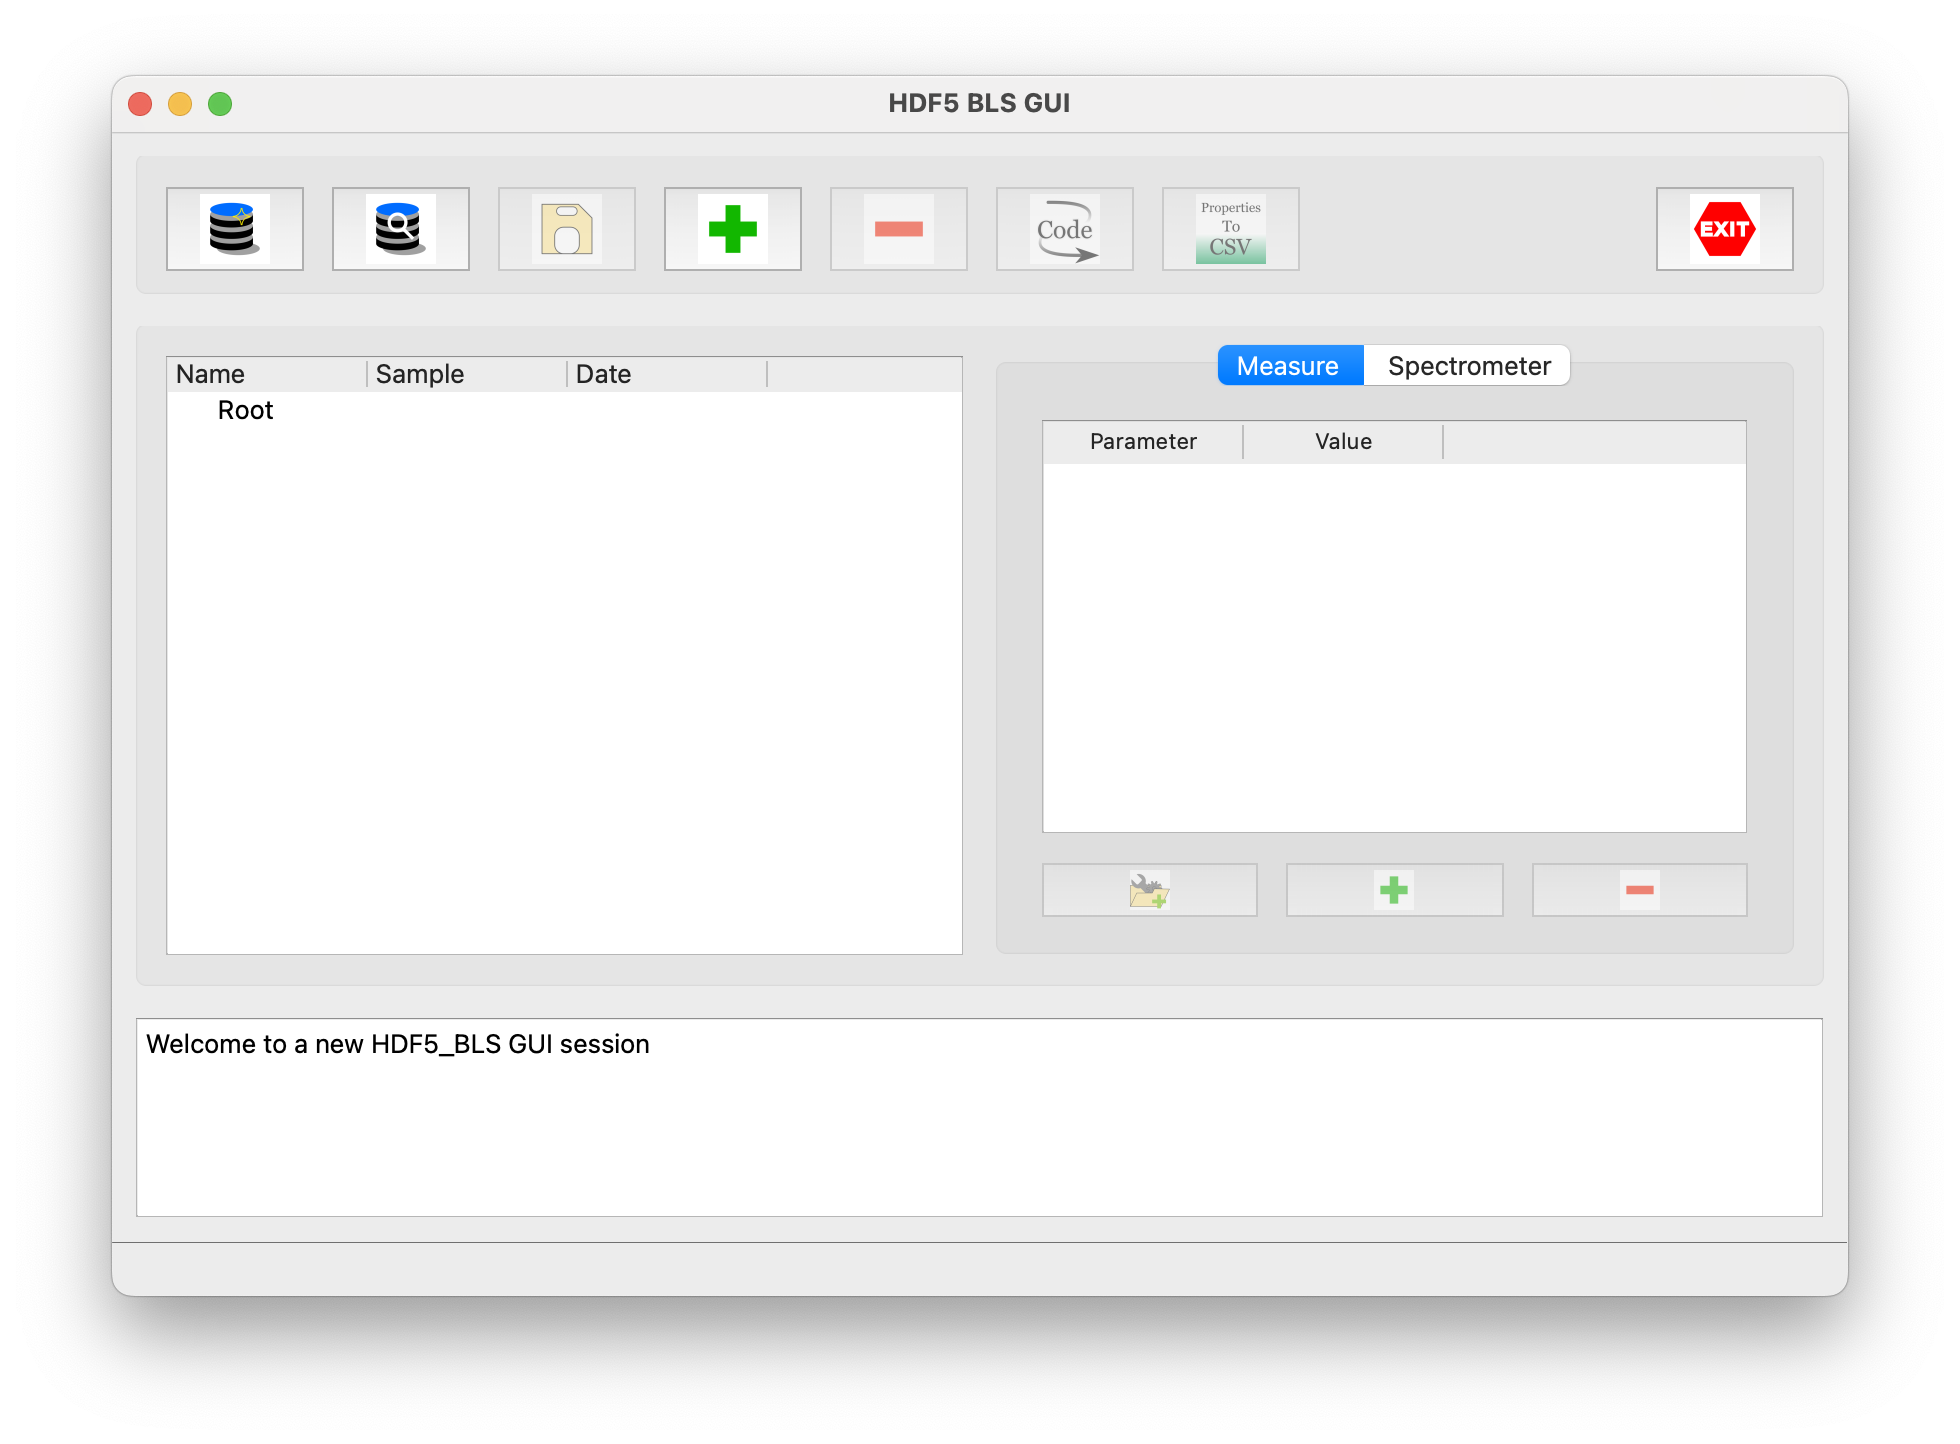
\includegraphics[width=\textwidth]{img/main_window.png}
    \caption{HDF5\_BLS\_GUI Main Window}
    \label{fig:gui_main_window}
\end{figure}

The window is divided into four main sections:
\begin{itemize}
    \item Top: Contains a series of buttons to perform actions on the HDF5 file. The buttons are divided into three categories.
    \item Left: Displays the hierarchical structure of the HDF5 file, allowing users to navigate through its contents.
    \item Right: Shows the properties and metadata of the selected HDF5 object, providing detailed information to the user.
    \item Bottom: Contains a logging area to display messages and information about the current operations.
\end{itemize}

The GUI also comes with left and right clicks capabilities. Left clicking on any item in the hierarchical structure will display its properties in the right panel, while right clicking will open a context menu with additional options. A double click on any of the properties of the right pannel will allow us to edit the property.

The GUI finally comes with a menu where all the properties are recapitulated as well as a few other options.

\section{Module structure}
    The HDF5\_BLS package is built around the following different modules:
\begin{itemize}
    \item \texttt{wrapper}: This module is used to interact with HDF5 files. It is used to read the data, to write the data and to modify any aspect of the HDF5 file (dataset, groups or attributes).
    \item \texttt{analyze}: This module is used to convert raw data taken from a spectrometer into a physically meaningful Power Spectral Density (PSD) array. This process is done to be reliable 
    \item \texttt{treat}: This module is used to extract information from the PSD array, such as the frequency shift and line width of the spectral lines. 
    \item \texttt{load\_data}: This module is used to import data from any formats of interest. This module is an interface between physical files stored on the PC and the wrapper module. It has been designed to be easily extended to any format of data.
\end{itemize}

In the following chapters, we will focus on the different modules.
 
        
    \chapter{Initialization of the Wrapper object - creating or opening a HDF5 file}
        \begin{tcolorbox}
\textit{IN A NUTSHELL:}
\begin{lstlisting}
wrp = Wrapper(filepath = "path/to/file.h5")
\end{lstlisting}
"path/to/file.h5" is the path where you want to store the file or where the file is stored.
\end{tcolorbox}


To initialize a Wrapper object after having imported the library, you can run the following command:
\begin{lstlisting}
wrp = Wrapper()
\end{lstlisting}

This will create a new Wrapper object with no attributes or data with the following structure:
\begin{verbatim}
    file.h5
    +-- Brillouin (group)
\end{verbatim}

By default, the attributes of the "Brillouin" group are the following:
\begin{verbatim}
    file.h5
    +-- Brillouin (group)
    |   +-- Brillouin_type -> "Root"
    |   +-- HDF5_BLS_version -> "0.1" 
\end{verbatim}

This file is stored temporarily in the library folder and is deleted when the Wrapper object is destroyed or when the file is stored elsewhere. It is therefore good practice to specify a non-temporary filepath to the file when creating a new Wrapper object, with the "filepath" parameter:
\begin{lstlisting}
wrp = Wrapper(filepath = "path/to/file.h5")
\end{lstlisting}
Note that this works both for new files, and for files that already exist, in the latter case, the wrapper object applies to the file located at "path/to/file.h5".


    \chapter{Adding arrays to the HDF5 file using the Wrapper object}
        \begin{tcolorbox}
\textit{IN A NUTSHELL:}
\begin{itemize}
    \item With the \hyperref[subsec:wrapper.add_dictionnary]{add\_dictionnary} method 
\begin{lstlisting}
wrp = Wrapper()
dic = {"Raw_data": {"Name": "Wonderful measure 019", 
                    "Data": np.random.random((100, 100))},
       "PSD": {"Name": "PSD extracted blabla", 
               "Data": np.random.random((100, 100))},
       "Frequency": {"Name": "The Frequency",   
                   "Data": np.random.random((100))},
       "Abscissa_t": {"Name": "Time (s)", 
                      "Data": np.random.random((100)),
                      "Unit": "s",
                      "Dim_start": "0",
                      "Dim_end": "1"}}
wrp.add_dictionnary(dic, 
                    parent_group = "Brillouin", 
                    name = "Data_0", 
                    brillouin_type = "Measure",
                    overwrite = False)
\end{lstlisting}
    \item With specific methods for each type of data:
    \begin{itemize}
        \item \hyperref[subsec:wrapper.add_raw_data]{add\_raw\_data}: To add raw data to a group
\begin{lstlisting}
wrp = Wrapper()
data = np.random.random((10, 10, 512)) # The raw data that you want to add
wrp.add_raw_data(data,
                parent_group = "Brillouin/Data_0", 
                name = "Raw_data")
\end{lstlisting}
        \item \hyperref[subsec:wrapper.add_psd]{add\_PSD}: To add a PSD to a group
\begin{lstlisting}
wrp = Wrapper()
data = np.random.random((10, 10, 512)) # The PSD that you want to add
wrp.add_PSD(data,
            parent_group = "Brillouin/Data_0", 
            name = "PSD")
\end{lstlisting}
        
\end{itemize}
\end{itemize}
\end{tcolorbox}
\begin{tcolorbox}
\begin{itemize}
    \item[] \begin{itemize}
        \item \hyperref[subsec:wrapper.add_frequency]{add\_frequency}: To add a frequency axis to a group
\begin{lstlisting}
wrp = Wrapper()
data = np.random.random((512)) # The frequency axis that you want to add
wrp.add_frequency(data,
                  parent_group = "Brillouin/Data_0", 
                  name = "Frequency")
\end{lstlisting}
        \item \hyperref[subsec:wrapper.add_abscissa]{add\_abscissa}: To add an abscissa to a group
\begin{lstlisting}
wrp = Wrapper()
data = np.random.random((10, 10)) # The abscissa that you want to add
wrp.add_abscissa(data,
                 parent_group = "Brillouin/Data_0", 
                 name = "x and y",
                 unit = "microns",
                 dimension_PSD_start = 0,
                 dimension_PSD_end = 1)
\end{lstlisting}
        \item \hyperref[subsec:wrapper.add_treated_data]{add\_treated\_data}: To add a shift, linewidth and their respective standard deviations to a dedicated "Treatment" group
\begin{lstlisting}
wrp = Wrapper()
shift = np.random.random((10, 10)) # The shift array to add
linewidth = np.random.random((10, 10)) # The linewidth array to add
shift_std = np.random.random((10, 10)) # The shift standard deviation array to add
linewidth_std = np.random.random((10, 10)) # The linewidth standard deviation array to add
wrp.add_treated_data(shift = shift,
                     linewidth = linewidth,
                     shift_std = shift_std,
                     linewidth_std = linewidth_std,
                     parent_group = "Brillouin/Data_0", 
                     name_group = "NnMF - 5GHz")
\end{lstlisting}
    \end{itemize}
\end{itemize}
\end{tcolorbox}

Adding datasets to the HDF5 file through the HDF5\_BLS package is always handled by the \hyperref[subsec:wrapper.add_dictionnary]\texttt{Wrapper.add\_dictionnary} method. This method is complex and not user-friendly. There are therefore other derived methods that are meant to simplify the process of adding data to the HDF5 file, specific to each type of data.

In this tutorial, we present only the derived methods that are specific to each type of data. To get a better understanding on how to use the add\_dictionnary method, please refer to the \hyperref[subsec:wrapper.add_dictionnary]{developper guide section}.

To add a single dataset to a group, we first need to specify the type of dataset we want to add, following the ones presented in \hyperref[subsec:preamble.file_structure.complete_structure]{preamble}:
\begin{itemize}
    \item "Abscissa\_...": An abscissa array for the measures (time, position, ...)
    \item "Frequency": A Frequency dataset associated to the PSD dataset
    \item "PSD": A Power Spectral Density dataset
    \item "Raw\_data": A dataset that is not yet a PSD (for example the measure coming out of a VIPA spectrometer)
    \item "Shift": A shift array
    \item "Shift\_std": The standard deviation of the shift array
    \item "Linewidth": A linewidth array
    \item "Linewidth\_std": The standard deviation of the linewidth array
\end{itemize}

From there, 5 functions are available to add the dataset to the HDF5 file:
\begin{itemize}
    \item \hyperref[subsec:wrapper.add_raw_data]{add\_raw\_data}: To add raw data to a group
    \item \hyperref[subsec:wrapper.add_psd]{add\_PSD}: To add a PSD to a group
    \item \hyperref[subsec:wrapper.add_frequency]{add\_frequency}: To add a frequency axis to a group
    \item \hyperref[subsec:wrapper.add_abscissa]{add\_abscissa}: To add an abscissa to a group
    \item \hyperref[subsec:wrapper.add_treated_data]{add\_treated\_data}: To add a shift, linewidth and their respective standard deviations to a dedicated "Treatment" group
\end{itemize}

We have decided to separate the addition of a PSD and a Frequency array as in some setups, the Frequency array can be common to a range of experiments, like when a TFP is used.

All these functions have the same approach to the process of adding a dataset to a group:

\begin{figure}[H]
    \centering
    \label{fig:wrapper.flowchart_add_functions}
    \small
    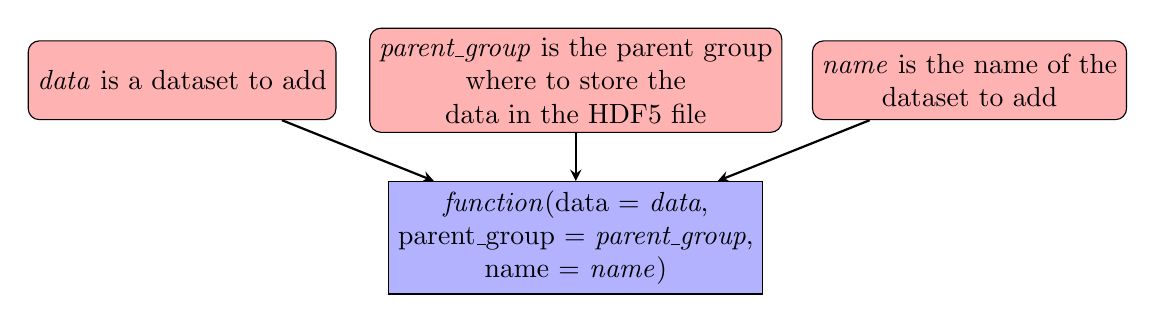
\begin{tikzpicture}[node distance=2cm]
        \node (start) [startstop] {\textit{data} is a dataset to add};
        \node (parentGroup) [startstop, right of=start, yshift=0cm, xshift=3cm, align=center] {\textit{parent\_group} is the parent group \\ where to store the \\data in the HDF5 file};
        \node (name) [startstop, right of=parentGroup, yshift=0cm, xshift=3cm, align=center] {\textit{name} is the name of the \\dataset to add};
        \node (function) [process, below of=parentGroup, yshift=0cm, xshift=0cm, align=center] {\textit{function}(data = \textit{data}, \\parent\_group = \textit{parent\_group}, \\name = \textit{name})};

        \draw [arrow] (start) -- (function);
        \draw [arrow] (parentGroup) -- (function);
        \draw [arrow] (name) -- (function);
    \end{tikzpicture}
    \caption{Flowchart of the get\_attributes method}
\end{figure}

This approach totally explains the definition of \hyperref[subsec:wrapper.add_raw_data]{add\_raw\_data}, \hyperref[subsec:wrapper.add_psd]{add\_PSD} and \hyperref[subsec:wrapper.add_frequency]{add\_frequency} methods. We'll see later how this logic had to be modified to add abscissa and treated data.

\begin{center}
    \rule{15cm}{0.4pt}
\end{center}

\paragraph{Example}
Let's consider the following example: we have just initialized a wrapper object and want to add a spectrum obtained from our spectrometer. We have already converted this spectrum to a numpy array, and named it \textit{data}. Now we want to add this data in a group called "Water spectrum" in the root group of the HDF5 file and call this raw data "Measure of the year". Then we will write:
\begin{lstlisting}
wrp.add_raw_data(data = data,
                 parent_group = "Brillouin/Water spectrum", 
                 name = "Measure of the year")
\end{lstlisting}

Now let's say that we have analyzed this spectrum and obtained a PSD (stored in the variable "psd") and frequency array (stored in the variable "freq"). We want to add these two arrays in the same group, and call them "PSD" and "Frequency" respectively. We will write:
\begin{lstlisting}
wrp.add_PSD(data = psd,
            parent_group = "Brillouin/Water spectrum", 
            name = "PSD")
wrp.add_frequency(freq,
                  parent_group = "Brillouin/Water spectrum", 
                  name = "Frequency")
\end{lstlisting}

\begin{center}
    \rule{15cm}{0.4pt}
\end{center}


Now for adding abscissa and treated data, we need to improve our approach. For abscissa, we need to be able to specify the dimension of the PSD and treated arrays to which the abscissa corresponds to and the unit of the axis. For treated data, we need to add more than just one dataset to the group. 

Let's look at the flowchart describing how to use the \hyperref[subsec:wrapper.add_abscissa]{add\_abscissa} method:

\begin{figure}[H]
    \centering
    \label{fig:wrapper.flowchart_add_abscissa}
    \small
    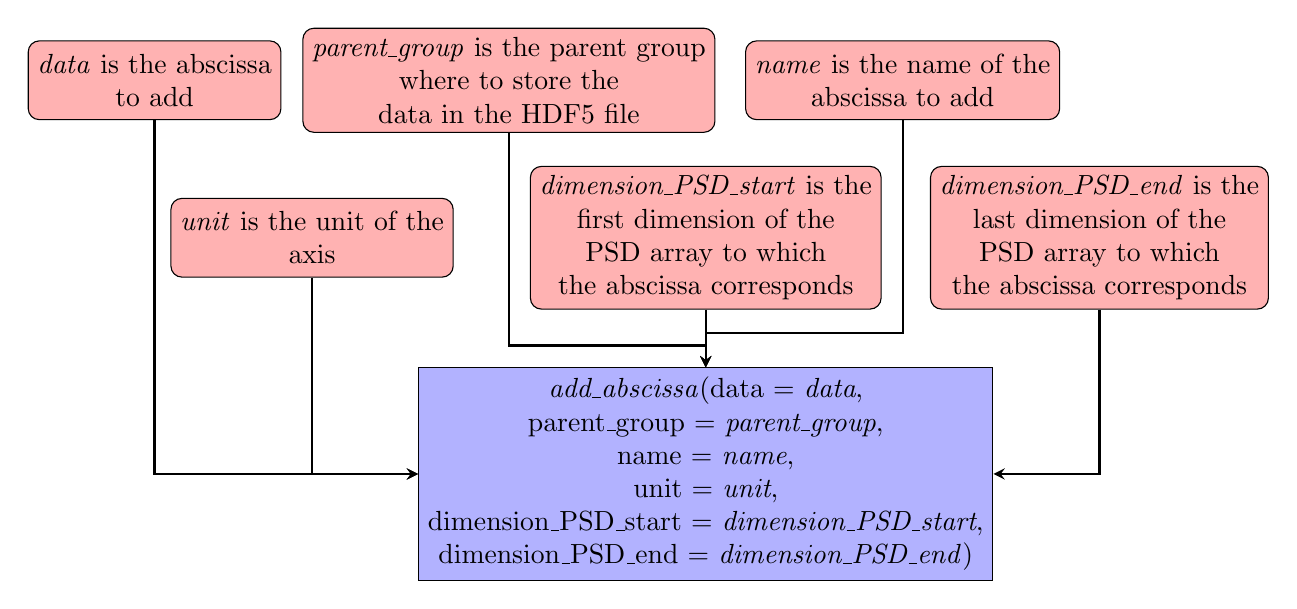
\begin{tikzpicture}[node distance=2cm]
        \node (start) [startstop, align=center] {\textit{data} is the abscissa\\ to add};
        \node (parentGroup) [startstop, right of=start, yshift=0cm, xshift=2.5cm, align=center] {\textit{parent\_group} is the parent group \\ where to store the \\data in the HDF5 file};
        \node (name) [startstop, right of=parentGroup, yshift=0cm, xshift=3cm, align=center] {\textit{name} is the name of the \\abscissa to add};
        \node (unit) [startstop, below of=start, yshift=0cm, xshift=2cm, align=center] {\textit{unit} is the unit of the \\axis};
        \node (dimensionPSD) [startstop, right of=unit, yshift=0cm, xshift=3cm, align=center] {\textit{dimension\_PSD\_start} is the\\ first dimension of the \\PSD array to which\\ the abscissa corresponds};
        \node (dimensionPSD_end) [startstop, right of=dimensionPSD, yshift=0cm, xshift=3cm, align=center] {\textit{dimension\_PSD\_end} is the\\ last dimension of the \\PSD array to which \\the abscissa corresponds};            
        \node (function) [process, below of=dimensionPSD, yshift=-1cm, xshift=0cm, align=center] {\textit{add\_abscissa}(data = \textit{data}, \\parent\_group = \textit{parent\_group}, \\name = \textit{name}, \\unit = \textit{unit}, \\dimension\_PSD\_start = \textit{dimension\_PSD\_start}, \\dimension\_PSD\_end = \textit{dimension\_PSD\_end})};

        \draw [arrow] (start) |- (function);
        \draw [arrow] ++(parentGroup.south) |- +(0cm, -2.7cm) -| (function.north);
        \draw [arrow] ++(name.south) |- +(0cm, -2.7cm) -| (function.north);            
        \draw [arrow] (unit) |- (function);
        \draw [arrow] (dimensionPSD) -- (function);
        \draw [arrow] (dimensionPSD_end) |- (function);
    \end{tikzpicture}   
    \caption{Flowchart of the add\_abscissa method}
\end{figure}

\begin{center}
    \rule{15cm}{0.4pt}
\end{center}

\paragraph{Example}
Let's consider the following example: we have just initialized a wrapper object and want to add an abscissa axis corresponding to our measures that have been stored in the group "Brillouin/Temp". Say that this abscissa axis corresponds to temperature values, from 35 to 40 degrees and that there are 10 points in the axis. We will therefore call this abscissa axis "Temperature". We will write:
\begin{lstlisting}
wrp.add_abscissa(data = np.linspace(35, 40, 10),
                 parent_group = "Brillouin/Temp", 
                 name = "Temperature",
                 unit = "C",
                 dim_start = 0,
                 dim_end = 1)
\end{lstlisting}

Of course if you want to import saved values for this axis, you can also specify them directly in the function call:
\begin{lstlisting}
wrp.add_abscissa(data = data,
                 parent_group = "Brillouin/Temp", 
                 name = "Temperature",
                 unit = "C",
                 dim_start = 0,
                 dim_end = 1)
\end{lstlisting}

\begin{center}
    \rule{15cm}{0.4pt}
\end{center}

Now, for adding treated data (that is the shift, linewidth and their standard deviations), the flowchart of the \hyperref[subsec:wrapper.add_treated_data]{add\_treated\_data} method becomes:

\begin{figure}[H]
    \centering
    \label{fig:wrapper.flowchart_add_treat}
    \small
    \begin{tikzpicture}[node distance=2cm]
        \node (start) [startstop, align=center] {\textit{shift} is the shift\\ array to add};
        \node (parentGroup) [startstop, right of=start, yshift=0cm, xshift=2.5cm, align=center] {\textit{parent\_group} is the parent group \\ where to store the \\data in the HDF5 file};
        \node (name) [startstop, right of=parentGroup, yshift=0cm, xshift=3cm, align=center] {\textit{name} is the name of the \\abscissa to add};
        \node (linewidth) [startstop, below of=start, yshift=0cm, xshift=2cm, align=center] {\textit{linewidth} is thelinewidth\\ array to add};
        \node (shiftSTD) [startstop, right of=linewidth, yshift=0cm, xshift=3cm, align=center] {\textit{shift\_std} is the\\ standard deviation of\\ the shift array};
        \node (linewidthSTD) [startstop, right of=shiftSTD, yshift=0cm, xshift=3cm, align=center] {\textit{linewidth\_std} is the\\ standard deviation of\\ the linewidth array};            
        \node (function) [process, below of=dimensionPSD, yshift=-1cm, xshift=0cm, align=center] {\textit{add\_treated\_data}(shift = \textit{shift}, \\ linewidth = \textit{linewidth}, \\shift\_std = \textit{shift\_std}, \\linewidth\_std = \textit{linewidth\_std},\\ parent\_group = \textit{parent\_group}, \\name = \textit{name})};

        \draw [arrow] (start) |- (function);
        \draw [arrow] ++(parentGroup.south) |- +(0cm, -2.7cm) -| (function.north);
        \draw [arrow] ++(name.south) |- +(0cm, -2.7cm) -| (function.north);            
        \draw [arrow] (linewidth) |- (function);
        \draw [arrow] (shiftSTD) -- (function);
        \draw [arrow] (linewidthSTD) |- (function);
    \end{tikzpicture}   
    \caption{Flowchart of the add\_abscissa method}
\end{figure}


\begin{center}
    \rule{15cm}{0.4pt}
\end{center}

\paragraph{Example}
Let's consider the following example: we have treated our data and have obtained a shift array (shift), a linewidth array (linewidth) and their standard deviations (shift\_std and linewidth\_std). We want to add these arrays in the same group as the PSD, that is the group "Test". The treated data are stored in a separate group nested in the "Test" group by the choices made while building the structure of the file. This is so the name of the treatment group can be chosen freely. Let's say that in this case, we have performed a non-negative matrix factorization (NnMF) on the data, and extracted the shift values closest to 5GHz. We will therefore call this treatment "NnMF - 5GHz". We will write:
\begin{lstlisting}
wrp.add_treated_data(shift = shift,
                     linewidth = linewidth,
                     shift_std = shift_std,
                     linewidth_std = linewidth_std,
                     parent_group = "Brillouin/Test", 
                     name_group = "NnMF - 5GHz")
\end{lstlisting}

\begin{center}
    \rule{15cm}{0.4pt}
\end{center}

    \chapter{Importing data to the HDF5 file using the Wrapper object}
        \begin{tcolorbox}
    \textit{IN A NUTSHELL:}

    Importing data from files is done with specific methods for each type of data that is imported:
    \begin{itemize}
        \item \hyperref[subsec:wrapper.import_abscissa]{Wrapper.import\_abscissa}: To import an abscissa from a measure file.
\begin{lstlisting}
    wrp = Wrapper()
    wrp.import_abscissa(filepath = "path/to/file.txt", parent_group = "Brillouin/Measure", creator = None, parameters = None, name = "Time", unit = "s", dim_start = 0, dim_end = 1, reshape = None, overwrite = False)
\end{lstlisting}
        \item \hyperref[subsec:wrapper.import_frequency]{Wrapper.import\_frequency}: To import a frequency array from a measure file.
\begin{lstlisting}
    wrp.import_frequency(filepath = "path/to/file.txt", parent_group = "Brillouin/Measure", creator = None, parameters = None, name = "Frequency", reshape = None, overwrite = False)
\end{lstlisting}
        \item \hyperref[subsec:wrapper.import_psd]{Wrapper.import\_PSD}: To import a Power Spectral Density array from a measure file.
\begin{lstlisting}
    wrp.import_PSD(filepath = "path/to/file.txt", parent_group = "Brillouin/Measure", creator = None, parameters = None, name = "PSD", reshape = None, overwrite = False)
\end{lstlisting}
        \item \hyperref[subsec:wrapper.import_raw_data]{Wrapper.import\_raw\_data}: To import a Raw data array from a measure file.
\begin{lstlisting}
    wrp.import_raw_data(filepath = "path/to/file.txt", parent_group = "Brillouin/Measure", creator = None, parameters = None, name = "PSD", reshape = None, overwrite = False)
\end{lstlisting}
        \item \hyperref[subsec:wrapper.import_treated_data]{Wrapper.import\_treated\_data}: To import the data arrays resulting from a treatment.
\begin{lstlisting}
    wrp.import_treated_data(self, filepath_shift, filepath_linewidth, filepath_shift_std, filepath_linewidth_std, parent_group, creator = None, parameters = None, name = None, reshape = None, overwrite = False):
\end{lstlisting}
    \end{itemize}

    \textbf{Note:} Importing the data is done using the load\_data module. All the data format and extensions handled by the module are described in the \hyperref[chap:load_data]{load\_data section}.
\end{tcolorbox}
    
\section{An overview}
    
    Importing datasets to the HDF5 file from independent data files, through the HDF5\_BLS package, is always done following to successive steps:
    \begin{enumerate}
        \item Extracting the data and the metadata that can be extracted from the data files. This is done using the \hyperref[chap:load_data]{load\_data module}.
        \item Adding the data and metadata to the HDF5 file. This is done using the \hyperref[subsec:wrapper.add_dictionnary]{Wrapper.add\_dictionnary} method.
    \end{enumerate}

    To make the process more user friendly, we have developed a set of derived methods that are specific to each type of data that is to be added (Raw data, PSD, Frequency, Abscissa or treated data). 

\section{The logic behind the adding functions}
    Following the same approach as described in the previous chapter, we import data in function of their nature, using dedicated functions. These functions are:
    \begin{itemize}
        \item \hyperref[subsec:wrapper.import_abscissa]{Wrapper.import\_abscissa}: To import an abscissa array.
        \item \hyperref[subsec:wrapper.import_frequency]{Wrapper.import\_frequency}: To import a frequency array.
        \item \hyperref[subsec:wrapper.import_psd]{Wrapper.import\_PSD}: To import a PSD array.
        \item \hyperref[subsec:wrapper.import_raw_data]{Wrapper.import\_raw\_data}: To import raw data.
        \item \hyperref[subsec:wrapper.import_treated_data]{Wrapper.import\_treated\_data}: To import the data arrays resulting from a treatment.
    \end{itemize}

    The logic behind the import functions is the following:
    \begin{figure}[H]
        \centering
        \label{fig:wrapper.flowchart_import_functions}
        \small
        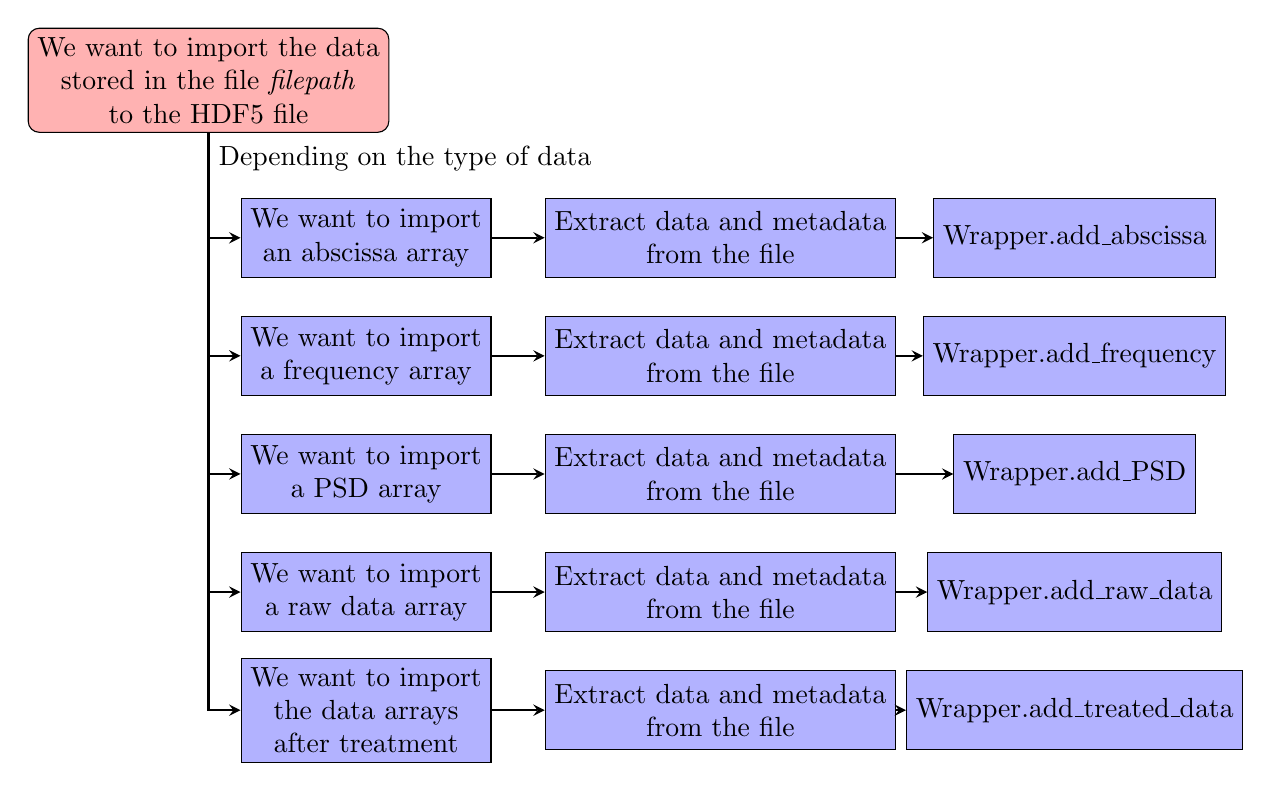
\begin{tikzpicture}[node distance=1cm]
            \node (start) [startstop, align=center] {We want to import the data\\stored in the file \textit{filepath}\\to the HDF5 file};
            \node(isAbscissa) [process, below of=start, yshift=-1cm, xshift=2cm, align=center] {We want to import\\an abscissa array};
            \node(isFreq) [process, below of=isAbscissa, yshift=-0.5cm, xshift=0cm, align=center] {We want to import\\a frequency array};
            \node(isPSD) [process, below of=isFreq, yshift=-0.5cm, xshift=0cm, align=center] {We want to import\\a PSD array};
            \node(israw) [process, below of=isPSD, yshift=-0.5cm, xshift=0cm, align=center] {We want to import\\a raw data array};
            \node(isTreated) [process, below of=israw, yshift=-0.5cm, xshift=0cm, align=center] {We want to import\\the data arrays\\after treatment};
            \node(extAbs) [process, right of=isAbscissa, yshift=0cm, xshift=3.5cm, align=center] {Extract data and metadata\\from the file};
            \node(extFreq) [process, right of=isFreq, yshift=0cm, xshift=3.5cm, align=center] {Extract data and metadata\\from the file};
            \node(extPSD) [process, right of=isPSD, yshift=0cm, xshift=3.5cm, align=center] {Extract data and metadata\\from the file};
            \node(extraw) [process, right of=israw, yshift=0cm, xshift=3.5cm, align=center] {Extract data and metadata\\from the file};
            \node(extTreated) [process, right of=isTreated, yshift=0cm, xshift=3.5cm, align=center] {Extract data and metadata\\from the file};
            \node(fAbs) [process, right of=extAbs, yshift=0cm, xshift=3.5cm, align=center] {Wrapper.add\_abscissa};
            \node(fFreq) [process, right of=extFreq, yshift=0cm, xshift=3.5cm, align=center] {Wrapper.add\_frequency};
            \node(fPSD) [process, right of=extPSD, yshift=0cm, xshift=3.5cm, align=center] {Wrapper.add\_PSD};
            \node(fraw) [process, right of=extraw, yshift=0cm, xshift=3.5cm, align=center] {Wrapper.add\_raw\_data};
            \node(fTreated) [process, right of=extTreated, yshift=0cm, xshift=3.5cm, align=center] {Wrapper.add\_treated\_data};

            \draw[arrow] (start) |- node[anchor=west, yshift=1cm] {Depending on the type of data} (isAbscissa);
            \draw[arrow] (start) |- (isFreq);
            \draw[arrow] (start) |- (isPSD);
            \draw[arrow] (start) |- (israw);
            \draw[arrow] (start) |- (isTreated);
            \draw[arrow] (isAbscissa) -- (extAbs);
            \draw[arrow] (isFreq) -- (extFreq);
            \draw[arrow] (isPSD) -- (extPSD);
            \draw[arrow] (israw) -- (extraw);
            \draw[arrow] (isTreated) -- (extTreated);
            \draw[arrow] (extAbs) -- (fAbs);
            \draw[arrow] (extFreq) -- (fFreq);
            \draw[arrow] (extPSD) -- (fPSD);
            \draw[arrow] (extraw) -- (fraw);
            \draw[arrow] (extTreated) -- (fTreated);    
        \end{tikzpicture}
        \caption{Flowchart of the import functions}
    \end{figure}

\section{The arguments of the import functions}
    The import functions combine both the arguments needed for the "add\_" functions and the arguments needed to extract the data and metadata from the files. These are the following arguments:
    \begin{itemize}
        \item \textbf{filepath}: The path to the file containing the data to import. Note that for the "Wrapper.import\_ treated\_data" function, there are 4 different files to import (for the fshift, the linewidth, the shift\_std and the linewidth\_std arrays).
        \item \textbf{parent\_group}: The path to the group or dataset where the data will be added in the form "Brillouin/Measure/...".
        \item \textbf{creator} \textit{(optional, default None)}: Some file extensions are not structured in the same way. Depending on how particular labs store their data, the "creator" argument can be used to specify the structure of the file that has to be loaded. In most cases, this argument is not used and can be left to None. If it however has to be used, a LoadError\_creator will be raised.
        \item \textbf{parameters} \textit{(optional, default None)}: The parameters that are to be used to import the data correctly. These parameters are specific to the techniques used to obtain the data. In most cases, this argument is not used and can be left to None. If it however has to be used, a LoadError\_parameters will be raised.
        \item \textbf{name} \textit{(optional, default None)}: The name that will be given to the dataset. If None, the name is set to whatever the type of data is (e.g. "Frequency").
        \item \textbf{reshape} \textit{(optional, default None)}: The new shape of the array. If None, the shape is not changed.    
        \item \textbf{overwrite} \textit{(optional, default False)}: If True, the attributes of the selected group or dataset are overwritten if they already exist in the file.
    \end{itemize}


    \chapter{Import or combinine HDF5 files using the Wrapper object}
        \begin{tcolorbox}
    \textit{IN A NUTSHELL:}

    There are two ways to import a HDF5 file into another HDF5 file using the \texttt{Wrapper} object:
    \begin{itemize}
        \item \textbf{Importing:} In that case, the HDF5 file that is imported is added to the current file in a new group with name the name of the added file. This is done using the \hyperref[subsec:wrapper.add_hdf5]{add\_hdf5} method:
\begin{lstlisting}
    wrp = Wrapper()
    wrp.add_hdf5(filepath = "path/to/file.h5", parent_group = "Brillouin")
\end{lstlisting}
        \item \textbf{Combining:} We can also combine two HDF5 files into a single one. This means that we create a new HDF5 file where all the groups under the "Brillouin" group of the two files will be stored under the "Brillouin" group of the resulting file. This is done using the \hyperref[subsec:wrapper.__add__]{\_\_add\_\_} dunder method, or simply with the "+" operator:
\begin{lstlisting}
    wrp1 = Wrapper()
    wrp2 = Wrapper()
    wrp = wrp1 + wrp2
\end{lstlisting}
    \end{itemize}
\end{tcolorbox}
    
Creating a new HDF5 file based on two existing ones can be done one of two ways depending on the desired end result.
\begin{itemize}
    \item The \hyperref[subsec:wrapper.__add__]{\_\_add\_\_} dunder metthod. If we want to combine two HDF5 files into a single one "plainly", for example if we are generating a new HDF5 after each measure, with this structure:
    \begin{verbatim}
    20250214_HVEC_03.h5
    +-- Brillouin (group)
    |   +-- 20250214_HVEC_02
    |   |   +-- Measure (dataset)
    \end{verbatim}
    and we already have a HDF5 file containing the data of the previous experiment:
    \begin{verbatim}
    20250214_HVEC.h5
    +-- Brillouin (group)
    |   +-- 20250214_HVEC_01
    |   |   +-- Measure (dataset)
    |   +-- 20250214_HVEC_02
    |   |   +-- Measure (dataset)
    \end{verbatim}
    We can simply add the first HDF5 file to the second one with:
\begin{lstlisting}
wrp1 = Wrapper(filepath = ".../20250214_HVEC.h5")
wrp2 = Wrapper(filepath = ".../20250214_HVEC_02.h5")
wrp = wrp1 + wrp2
\end{lstlisting}
    This will create a new HDF5 file with the following structure:
    \begin{verbatim}
    20250214_HVEC.h5
    +-- Brillouin (group)
    |   +-- 20250214_HVEC_01
    |   |   +-- Measure (dataset)
    |   +-- 20250214_HVEC_02
    |   |   +-- Measure (dataset)
    |   +-- 20250214_HVEC_03
    |   |   +-- Measure (dataset)
    \end{verbatim}
    \textbf{WARNING:} The new file is a temporary file, it would therefore be interesting to save it after the addition of the two files with:
\begin{lstlisting}
wrp.save_as_hdf5(filepath = wrp1.filepath)
\end{lstlisting}
    Note that from there, wrp1 and wrp will be the same as the wrapper does not store any data in memory but just acts as an access facilitator to the file.

    \item The \hyperref[subsec:wrapper.add_hdf5]{add\_hdf5} method. If we want to import the HDF5 as a new group, for example if we have this HDF5 file containing the data of a cell study:
    \begin{verbatim}
    Neuronal_cell_study.h5
    +-- Brillouin (group)
    |   +-- Neuronal (group)
    |   |   +-- GT 1-7 (group)
    |   |   |   +-- ...
    |   |   +-- L-fibroblast (group)
    |   |   |   +-- ...
    |   +-- Skeletal (group)
    |   |   +-- ...
    \end{verbatim}
    And we want to import data done on another neuronal cell line, say "MOV", that have been stored in the following HDF5 file:
    \begin{verbatim}
    MOV.h5
    +-- Brillouin (group)
    |   +-- MOV (group)
    |   |   +-- ...
    \end{verbatim}
    We can simply add the second HDF5 file to the first one by specifying the path to the second file in the \texttt{Wrapper.add\_hdf5} method:
\begin{lstlisting}
wrp1 = Wrapper(filepath = ".../Neuronal_cell_study.h5")
wrp1.add_hdf5(filepath = ".../MOV.h5", parent_group = "Brillouin/Neuronal")
\end{lstlisting}
    This will create a new HDF5 file with the following structure:
    \begin{verbatim}
    Neuronal_cell_study.h5
    +-- Brillouin (group)
    |   +-- Neuronal (group)
    |   |   +-- GT 1-7 (group)
    |   |   |   +-- ...
    |   |   +-- L-fibroblast (group)
    |   |   |   +-- ...
    |   |   +-- MOV (group)
    |   |   |   +-- ...
    |   +-- Skeletal (group)
    |   |   +-- ...
    \end{verbatim}
\end{itemize} 



\mypart{HDF5\_BLS GUI tutorial}
    \chapter{GUI quick start guide}
        To get started, you need to install the repository. Follow the instructions below:

\begin{itemize}
    \item Step 1: Make sure you have Python 3.10 or higher installed. You can download Python at \href{https://www.python.org/downloads/}{this link}.
    \item Step 2: Clone the repository at \href{https://github.com/bio-brillouin/HDF5_BLS/tree/main}{this link}.    
    \item Step 3: Create a virtual environment and install the requirements. To do so, open a terminal, navigate to the repository folder and install the requirements. For windows users, you can open the terminal into the cloned and extracted repository (shift+left click over the folder -> Open in terminal) and use the following command:
\begin{lstlisting}
python -m venv venv
.\venv\Scripts\activate
pip install -r requirements.txt
\end{lstlisting}
    For Mac users, you can navigate to the repository, make sure you can view the path bar at the bottom of Finder (if not, check View/Show Path Bar in the menu bar), then press control and left click on the folder and select "Open in Terminal". Then, use the following command:
\begin{lstlisting}
python -m venv venv
source venv/bin/activate
pip install -r requirements.txt
\end{lstlisting}
    For Linux users, you can navigate to the repository, open a terminal in the folder and use the same command as for Mac users.
    \item Step 4: Run the \texttt{HDF5\_BLS\_GUI/main.py} file with
\begin{lstlisting}
python HDF5\_BLS\_GUI/main.py
\end{lstlisting}
\end{itemize}

    \chapter{First Steps}
        \section{Creating a new file}
            After running all these steps, you should see the following window:

\begin{center}
    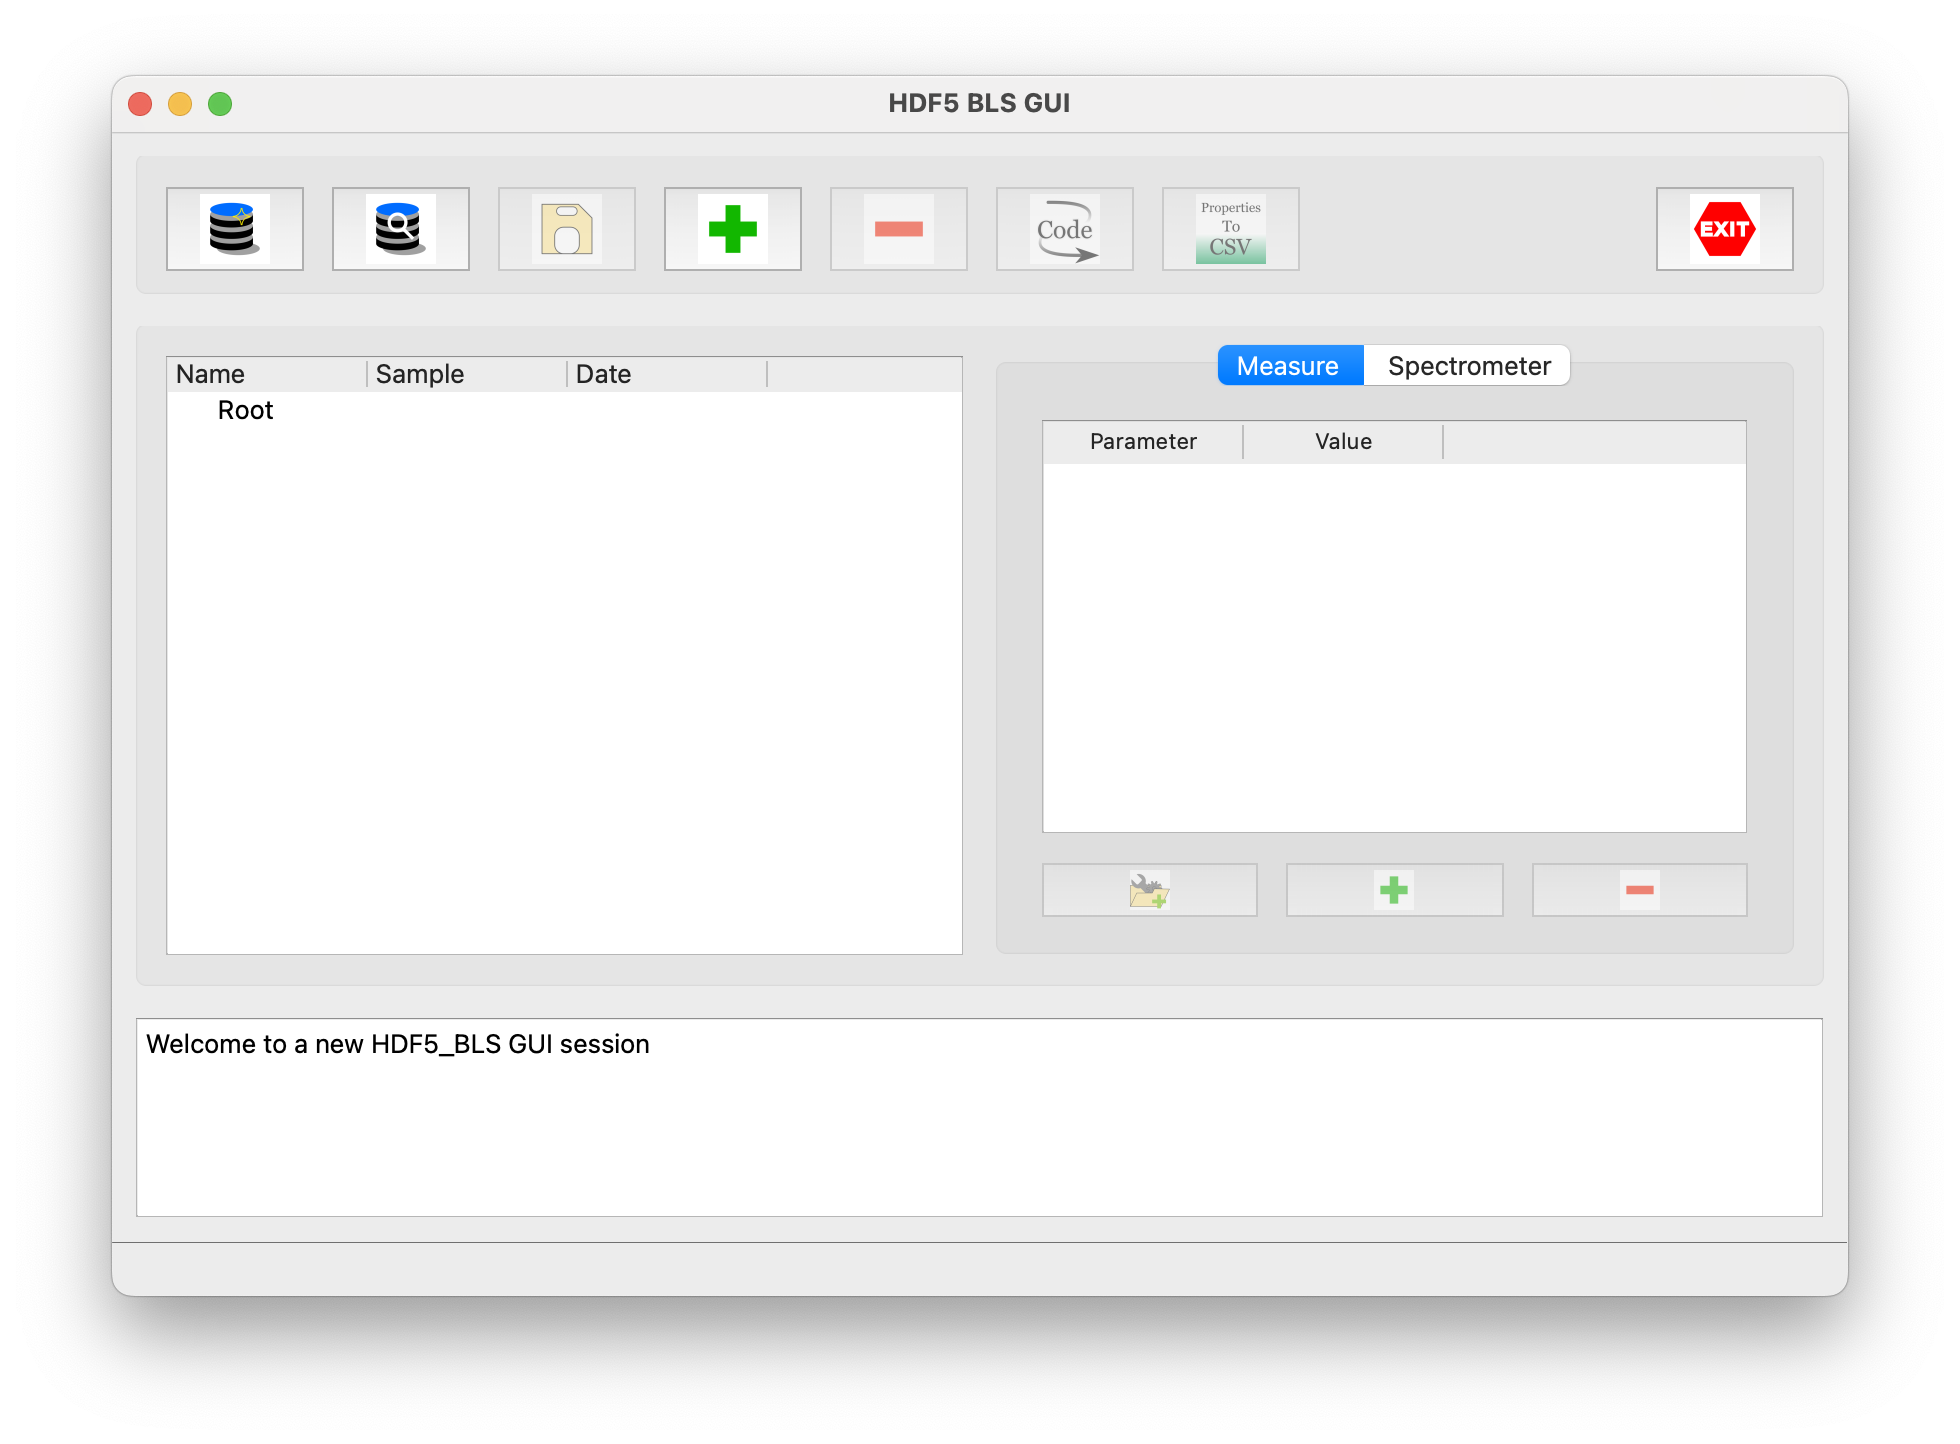
\includegraphics[width=\textwidth]{img/main_window.png}
\end{center}

You can then drag and drop your data into the left pannel and structure it as you wish. 

You can also add properties to your data in the form of a standard CSV file which model can be found in the \texttt{spreadsheets} folder of the repository. To add a new property file to your measure, select your measure on the left pannel and drag and drop your property file to the right pannel from a file viewer. 

Note that you can add property to a group of data. In that case, the property apply to all its elements.



\mypart{Development Guide} \label{chapter:dev_guide}
    \chapter{Wrapper}\label{sec:wrapper}
        \section{A little tour of the class}
            \begin{tcolorbox}
    The "Wrapper" class is the main class of the package. Its role is to interface the file and the software while ensuring a user-friendly access to the data and a conservation of the structure of the file. This class is meant to do these four actions:
    \begin{enumerate}
        \item Creates a structure that is universal to the BioBrillouin community in a seamless manner.
        \item Allow the user to acces the data and attributes of the file.
        \item Allow the user to add data to the file with attributes that are specific to the BioBrillouin community.
        \item Allow the user to add or modify attributes of the file.
    \end{enumerate}
\end{tcolorbox}

\paragraph{Memory management:}
HDF5 files are notorious for behing heavy. Storing a whole HDF5 file in flash memory is therefore generally a bad idea. As such, the "Wrapper" class works by accessing a file on the disk. By default this file is a temporary file stored in the project's directory. The class is however designed to work on existing HDF5 files stored in permanent locations.

\paragraph{Private attributes:} 
At initialization:
\begin{itemize}
    \item \textbf{self.filepath}: The path to the HDF5 file. By default, the path to the temporary file is used.
    \item \textbf{self.save}: A boolean that indicates whether the file has been saved or is still in the temporary file.
\end{itemize}

\paragraph{Dunders:} 
The "Wrapper" class has the following dunder methods that are described in the following sections:
\begin{itemize}
    \item \hyperref[subsec:wrapper.__init__]{Wrapper.\_\_init\_\_ -> Wrapper()}: The method that initializes the object
    \item \hyperref[subsec:wrapper.__getitem__]{Wrapper.\_\_getitem\_\_ -> Wrapper[key]}: The preferred method to access an element located at a given path, it allows to access an element by placing its path in the brackets of the "Wrapper" object.
    \item \hyperref[subsec:wrapper.__add__]{Wrapper.\_\_add\_\_ -> Wrapper + Wrapper}: A magic command to merge two wrappers together. It merges the contents of the "Brillouin" group.
\end{itemize}

\paragraph{Main Methods:} 
The "Wrapper" class has a number of methods that will be described in the following sections. The construction of the object has been done with a bottleneck strategy, where the critical interactions with the file are done with these methods:
\begin{itemize}
    \item \hyperref[subsec:wrapper.add_hdf5]{add\_hdf5}: A method to populate the file from a HDF5 file.
    \item \hyperref[subsec:wrapper.add_dictionnary]{add\_dictionnary}: A method to populate the file from a dictionnary.
    \item \hyperref[subsec:wrapper.create_group]{create\_group}: A method to create a new group inside the HDF5 file.
    \item \hyperref[subsec:wrapper.delete_element]{delete\_element}: A method to delete a dataset or group in the HDF5 file.
    \item \hyperref[subsec:wrapper.get_attributes]{get\_attributes}: A method to extract the attributes of a group or dataset.
    \item \hyperref[subsec:wrapper.get_structure]{get\_structure}: A method to extract the structure of the file.
    \item \hyperref[subsec:wrapper.save_as_hdf5]{save\_as\_hdf5}: A method to save the file to a desired location.
    \item \hyperref[subsec:wrapper.set_attributes_data]{set\_attributes\_data}: A method to set the attributes of a group or dataset.
\end{itemize}

\paragraph{Derived Methods:} 
To simplify however the creation and use of the file, these other methods also exist:
\begin{itemize}
    \item \hyperref[subsec:wrapper.add_abscissa]{add\_abscissa}: A method to add an abscissa arrayto the file.
    \item \hyperref[subsec:wrapper.add_frequency]{add\_frequency}: A method to add a frequency array to the file.
    \item \hyperref[subsec:wrapper.add_psd]{add\_psd}: A method to add a PSD to the file.
    \item \hyperref[subsec:wrapper.add_raw_data]{add\_raw\_data}: A method to add raw data to the file.
    \item \hyperref[subsec:wrapper.add_treated_data]{add\_treated\_data}: A method to add a shift, linewidth and their respective standard deviations to the file.
    \item \hyperref[subsec:wrapper.import_abscissa]{import\_abscissa}: A method to import an abscissa array to the file.
    \item \hyperref[subsec:wrapper.import_frequency]{import\_frequency}: A method to import a frequency array to the file.
    \item \hyperref[subsec:wrapper.import_psd]{import\_psd}: A method to import a PSD array to the file.
    \item \hyperref[subsec:wrapper.import_raw_data]{import\_raw\_data}: A method to import raw data to the file.
    \item \hyperref[subsec:wrapper.import_treated_data]{import\_treated\_data}: A method to import the data arrays resulting from a treatment.
    \item \hyperref[subsec:wrapper.import_properties_data]{import\_properties\_data}: A method to import the attributes of a dataset or group from a spreadsheet.
    \item \hyperref[subsec:wrapper.update_property]{update\_property}: A method to update the attributes of a dataset or group.
\end{itemize}

\paragraph{Console specific Methods:} 
Additionnaly, the "Wrapper" class has a few methods specifically to interact with the file from a terminal:
\begin{itemize}
    \item \hyperref[subsec:wrapper.print_structure]{print\_structure}: A method to print a tree view of the file in the terminal.
    \item \hyperref[subsec:wrapper.print_metadata]{print\_metadata}: A method to print all the attributes of a dataset or group at a given path in the terminal.
\end{itemize}

\paragraph{Wrapper Errors:}
The "Wrapper" class has a number of errors that can be raised by its methods:
\begin{itemize}
    \item \textbf{WrapperError\_StructureError}: Raised when a problem occurs with the structure of the file.
    \item \textbf{WrapperError\_FileNotFound}: Raised when a file stored in the disk is not found.
    \item \textbf{WrapperError\_Overwrite}: Raised when a group or dataset already exists in the file.
    \item \textbf{WrapperError\_ArgumentType}: Raised when the arguments given to the function are not of the expected type.
\end{itemize}
 
        
        \section{Dunder methods of the Wrapper class}
            \subsection{Wrapper.\_\_init\_\_ -> Wrapper()} \label{subchapter:wrapper.__init__}
    This magic command allows the user to initialize the wrapper. This dunder method is called with the following syntax:
\begin{lstlisting}
    wrp = Wrapper(filepath)
\end{lstlisting}

\paragraph{Attributes:}

\begin{itemize}
    \item \textbf{filepath}: \textit{optional, default None} The path to the HDF5 file. By default, a temporary file is created in the project's directory.
\end{itemize}

This method is called automatically when the "Wrapper" object is created. If it has to create a HDF5 file, it automatically creates the following structure:
\begin{verbatim}
    file.h5
    +-- Brillouin (group)
\end{verbatim}

By default, the attributes of the "Brillouin" group are the following:
\begin{verbatim}
    file.h5
    +-- Brillouin (group)
    |   +-- Brillouin_type -> "Root"
    |   +-- HDF5_BLS_version -> "1.0" # The version of the package
\end{verbatim}

If the file already exists, the wrapper object just stores the path to the file and does not overwrite it.

\subsection{Wrapper.\_\_getitem\_\_ -> Wrapper[key]} \label{subchapter:wrapper.__getitem__}
    This magic command allows the user to access an element located at a given path. This dunder method is called with the following syntax:
\begin{lstlisting}
    wrp["Brillouin/Measure/PSD"]
\end{lstlisting}

Of course, the path can be changed. 

If the path leads to a group, the entire group is returned as a closed group. If the path leads to a dataset, the dataset is returned as a numpy array.

\paragraph{Attributes:}

\begin{itemize}
    \item \textbf{path}: The path to the element to access in the form "Brillouin/Measure/PSD".
\end{itemize}

\paragraph{Raises:}

\begin{itemize}    
    \item \textbf{WrapperError\_StructureError}: Raises an error if the path does not lead to a valid element in the file.
\end{itemize}

\subsection{Wrapper.\_\_add\_\_ -> Wrapper + Wrapper} \label{subchapter:wrapper.__add__}
    This magic command allows the user to add two wrappers together. This dunder method is called with the following syntax:
\begin{lstlisting}
    new_wrapper = wrp1 + wrp2
\end{lstlisting}

In this example, wrp1 and wrp2 are two wrappers that are added together. The resulting wrapper is stored in the variable new\_wrapper. The addition of the two wrappers is done by adding the elements stored in the "Brillouin" group of both wrappers. The addition is possible only if the two wrappers have the same "HDF5\_BLS\_version" attribute. If the two wrappers have different "HDF5\_BLS\_version" attributes, the addition is not possible and an error is raised.

If you prefer to add a second wrapper to a dedicated group of the first wrapper, please use the \hyperref[subchapter:wrapper.add_hdf5]{Wrapper.add\_hdf5} method.

The addition of the two wrappers also affects the addition of attributes. Common attributes to all the groups will be set to the root group whereas attributes specific to each file will be set to their respective groups. Access to attributes is guaranteed by the \hyperref[subchapter:wrapper.get_attributes]{Wrapper.get\_attributes} method.

\paragraph{Attributes:}

\begin{itemize}
    \item \textbf{wrp2}: A wrapper to add to the current wrapper wrp1
\end{itemize}

\paragraph{Raises:}

\begin{itemize}
    \item \textbf{WrapperError\_FileNotFound}: If one of the two wrappers leads to a temporary file.
    \item \textbf{WrapperError\_StructureError}: If the two wrappers don't have the same version.
    \item \textbf{WrapperError\_Overwrite}: If the two wrappers share a group of same name.
    \item \textbf{WrapperError}: If an error occured while adding the data.
\end{itemize}

\begin{figure}[H]
    \centering
    \label{fig:wrapper.flowchart__add__}
    \small
    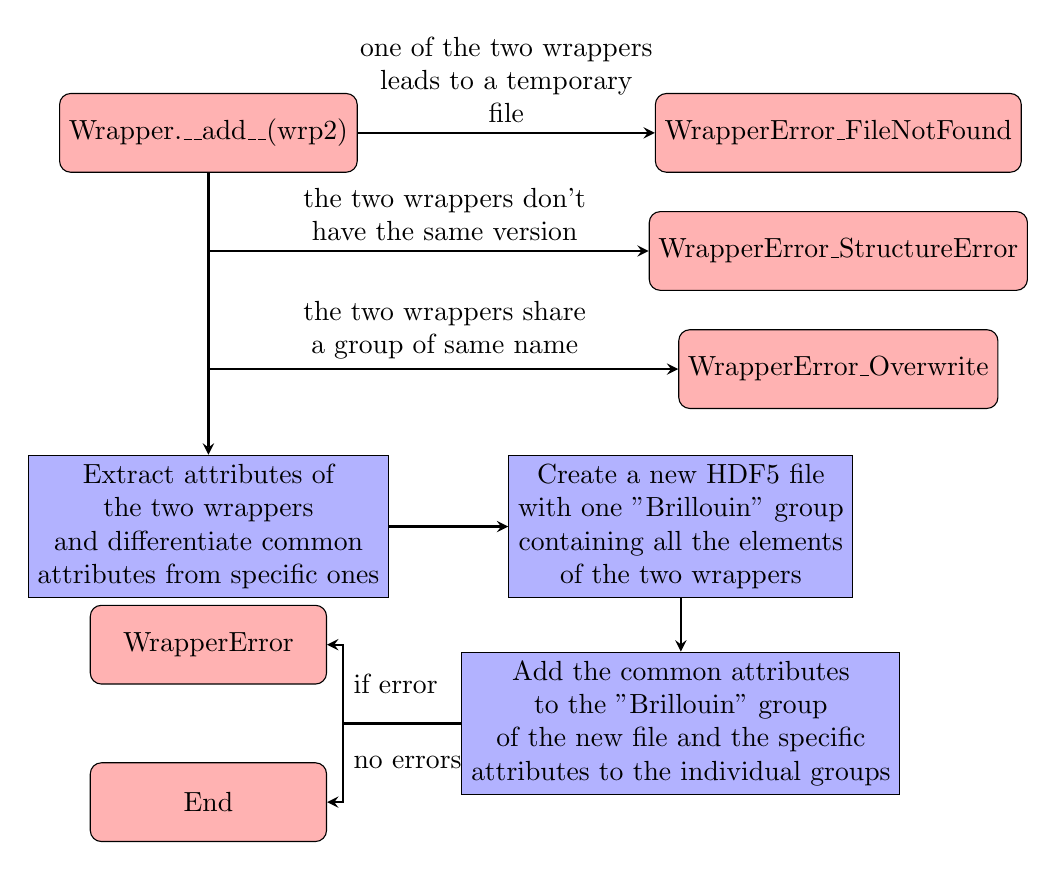
\begin{tikzpicture}[node distance=1cm]
        \node (start) [startstop, align=center] {Wrapper.\_\_add\_\_(wrp2)};
        \node (raiseError0) [startstop, right of=start, xshift=7cm] {WrapperError\_FileNotFound};
        \node (raiseError1) [startstop, below of=raiseError0, yshift=-0.5cm] {WrapperError\_StructureError};
        \node (raiseError2) [startstop, below of=raiseError1, yshift=-0.5cm] {WrapperError\_Overwrite};
        \node (manageAttributes) [process, below of=start, yshift=-4cm, align=center] {Extract attributes of\\ the two wrappers\\ and differentiate common\\ attributes from specific ones};
        \node (createFile) [process, right of=manageAttributes, xshift=5cm, align=center] {Create a new HDF5 file\\ with one "Brillouin" group\\ containing all the elements\\ of the two wrappers};
        \node (addAttributes) [process, below of=createFile, yshift=-1.5cm, align=center] {Add the common attributes\\ to the "Brillouin" group\\ of the new file and the specific\\ attributes to the individual groups};
        \node (raiseError3) [startstop, below of=manageAttributes, yshift=-0.5cm, align=center] {WrapperError};
        \node (end) [startstop, below of=raiseError3, yshift=-1cm, align=center] {End};

        \draw [arrow] (start) -- node[anchor=south, align=center] {one of the two wrappers\\ leads to a temporary\\file} (raiseError0);
        \draw [arrow] (start) |- node[anchor=south, align=center, xshift=3cm] {the two wrappers don't\\ have the same version} (raiseError1);
        \draw [arrow] (start) |- node[anchor=south, align=center, xshift=3cm] {the two wrappers share\\ a group of same name} (raiseError2);
        \draw [arrow] (start) -- (manageAttributes);
        \draw [arrow] (manageAttributes) -- (createFile);
        \draw [arrow] (createFile) -- (addAttributes);
        \draw [arrow] ++(addAttributes.west) -| +(-1.5cm, 0cm) |- node[anchor=west, align=center, yshift=-0.5cm] {if error} (raiseError3.east);
        \draw [arrow] ++(addAttributes.west) -| +(-1.5cm, 0cm) |- node[anchor=west, align=center, yshift=0.5cm] {no errors} (end);
        
    \end{tikzpicture}
    \caption{Flowchart of the \_\_add\_\_ method}
\end{figure}

        \section{Principal methods of the Wrapper class}
            % Main methods

\subsection{Wrapper.add\_hdf5} \label{subchapter:wrapper.add_hdf5}
    This method allows the user to add an HDF5 file to the file under a specific group. The group is created if it does not exist. The attributes of the HDF5 file are only added to the created group if they are different from the parent's attribute.

\begin{lstlisting}
def add_hdf5(self, filepath, parent_group = None, overwrite = False):
\end{lstlisting}

\paragraph{Attributes:}

\begin{itemize}
    \item \textbf{filepath}: The path to the HDF5 file to add.
    \item \textbf{parent\_group} \textit{(optional, default None)}: The parent group where to store the data of the HDF5 file, by default the parent group is the top group "Brillouin". The format of this group should be "Brillouin/Measure/...". 
    \item \textbf{overwrite} \textit{(optional, default False)}: If True, the group of same name than the HDF5 file that is added is overwritten. If False, only new attributes are added to the existing ones.
\end{itemize}

\paragraph{Returns:} Nothing

\paragraph{Raises:}

\begin{itemize}
    \item \textbf{WrapperError\_FileNotFound}: Raises an error if the filepath of the HDF5 file does not exist.
    \item \textbf{WrapperError\_StructureError}: Raises an error if the parent group does not exist in the HDF5 file.
    \item \textbf{WrapperError\_Overwrite}: Raises an error if the file name already exists in the selected group.
    \item \textbf{WrapperError}: Raises an error if the addition of the HDF5 file failed.
\end{itemize}

\paragraph{Flowchart:}

The function's logic is represented in the following flowchart:
\begin{figure}[H]
    \centering
    \label{fig:wrapper.flowchart_add_hdf5}
    \small
    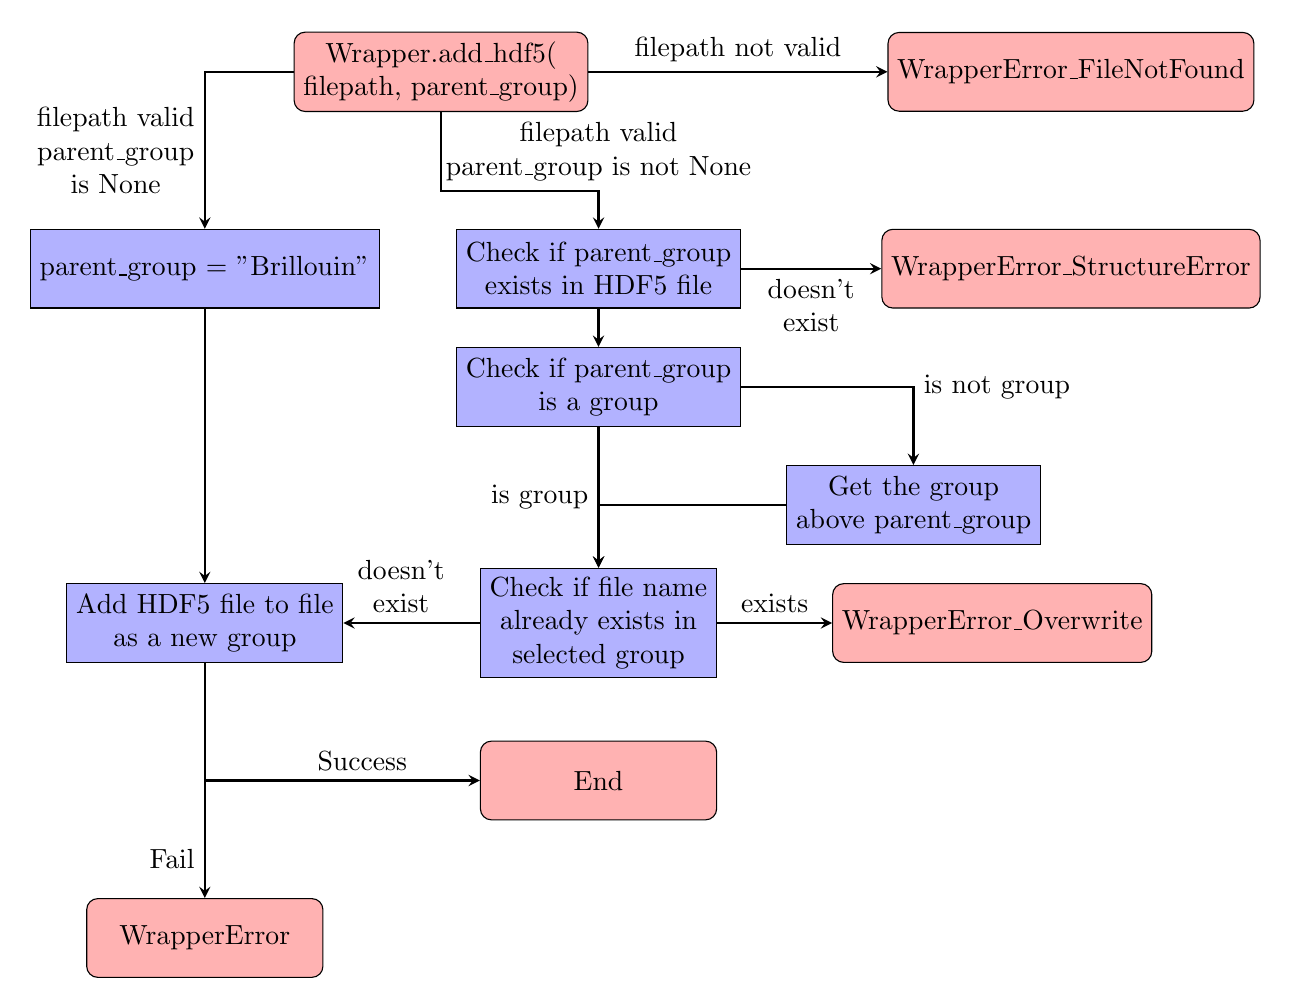
\begin{tikzpicture}[node distance=2cm]
        \node (start) [startstop, align=center] {Wrapper.add\_hdf5(\\filepath, parent\_group)};
        \node (raiseError0) [startstop, right of=start, xshift=6cm] {WrapperError\_FileNotFound};
        \node (setParent) [process, below of=start, yshift=-0.5cm, xshift=-3cm] {parent\_group = "Brillouin"};
        \node (checkExists) [process, right of=setParent, xshift=3cm, align=center] {Check if parent\_group\\ exists in HDF5 file};
        \node (raiseError1) [startstop, right of=checkExists, xshift=4cm] {WrapperError\_StructureError};
        \node (checkGroup) [process, below of=checkExists, yshift=0.5cm, align=center] {Check if parent\_group\\ is a group};
        \node (getGroup) [process, right of=checkGroup, yshift=-1.5cm, xshift = 2cm, align=center] {Get the group\\above parent\_group};
        \node (checkName) [process, below of=checkGroup, yshift=-1cm, align=center] {Check if file name\\  already exists in\\ selected group};
        \node (raiseError2) [startstop, right of=checkName, xshift=3cm] {WrapperError\_Overwrite};
        \node (addData) [process, below of=setParent, yshift=-2.5cm, align=center] {Add HDF5 file to file\\as a new group};
        \node (raiseError3) [startstop, below of=addData, yshift=-2cm] {WrapperError};
        \node (end) [startstop, below of=addData, xshift=5cm, yshift=0cm,] {End};

        \draw [arrow] (start) -- node[anchor=south] {filepath not valid} (raiseError0);
        \draw [arrow] (start) -| node[anchor=east, align=center, yshift=-1cm] {filepath valid \\ parent\_group \\is None} (setParent);
        \draw [arrow] ++(start.south) -- +(0mm, -1cm) -| node[anchor=south, align=center] {filepath valid \\ parent\_group is not None} (checkExists.north);
        \draw [arrow] (checkExists) -- node[anchor=north,align=center] {doesn't \\exist} (raiseError1);
        \draw [arrow] (checkExists) -- (checkGroup);
        \draw [arrow] (checkGroup) -- node[anchor=east] {is group} (checkName);
        \draw [arrow] (checkGroup) -| node[anchor=west] {is not group} (getGroup);
        \draw [arrow] (getGroup) -| (checkName);
        \draw [arrow] (checkName) -- node[anchor=south] {exists} (raiseError2);
        \draw [arrow] ++(checkName.west) -| +(-1cm, 0cm) |- node[anchor=south, align=center] {doesn't\\ exist} (addData.east);
        \draw [arrow] (setParent) -- (addData);
        \draw [arrow] (addData) |- node[anchor=south, align=center, xshift = 2cm] {Success} (end);
        \draw [arrow] (addData.south) -- node[anchor=east, yshift=-1cm] {Fail} (raiseError3.north);
    \end{tikzpicture}
    \caption{Flowchart of the add\_hdf5 method}
\end{figure}

% \subsection{Wrapper.add\_dictionnary} \label{subchapter:wrapper.add_dictionnary}
%     This method is the preferred way to add data to the wrapper. It allows the user to create a dictionary with the data and the attributes of the data he wants to add to the file. 

\begin{lstlisting}
def add_dictionnary(self, dic, parent_group = None, name_group = None, brillouin_type = "Measure", overwrite = False):
\end{lstlisting}

\paragraph{Attributes:}

\begin{itemize}
    \item \textbf{dic}: The dictionnary to add to the wrapper. This dictionnary has a preferred nomenclature for its keys that will allow the addition of the data with specific attributes to our file format. These keys are identical to the Brillouin\_types for dataset defined in \hyperref[subsec:preamble.file_structure.complete_structure]{preamble}. Each element of the dictionnary is another dictionnary with the following keys:
    \begin{itemize}
        \item "Name": The name of the dataset that will be stored. This can be any name that the user wants and find useful.
        \item "Data": The array that will be stored, or the dictionnary if we are adding attributes
        \item "Unit": \textit{Specific to "Abscissa\_..." keys}. The unit of the abscissa
        \item "Dim\_start": \textit{Specific to "Abscissa\_..." keys}. The first dimension to which the abscissa corresponds.
        \item "Dim\_end": \textit{Specific to "Abscissa\_..." keys}. The last dimension (excluded) to which the abscissa corresponds
    \end{itemize}
    \item \textbf{parent\_group} \textit{(optional, default None)}: The parent group where to store the data of the HDF5 file, by default the parent group is the top group "Brillouin". The format of this group should be "Brillouin/Measure/...". 
    \item \textbf{name\_group} \textit{(optional, default None)}: The name of the group where the elements of the dictionnary are stored. If None, the name is set to "Data\_i" where "i" is an integer that ensures that the name is unique. If the name already corresponds to a group, then the elements of the dictionnary are added in this group unless elements with same name already exist in the group or adding an element would result in more than one raw data in this group. 
    \item \textbf{brillouin\_type} \textit{(optional, default "Measure")}: The type of the group that will store the elements of the dictionnary. The possible values are the ones attributed to groups, defined earlier on in the \hyperref[subsec:preamble.file_structure.complete_structure]{preamble}
\end{itemize}

Here are typical examples of a dictionnary passed as attribute:
\begin{lstlisting}
dic_raw = {
    "Raw_data": {
        "Name": "Raw water spectrum", 
        "Data": np.array([...])}
} # a dictionnary with a raw data array straight from the spectrometer - for example if you want to do the whole anylisis process with the library.

dic_treated = {
    "Raw_data": {
        "Name": "Raw water spectrum", 
        "Data": np.array([...])}
    "PSD": {
        "Name": "PSD water TFP", 
        "Data": np.array([...])},
    "Frequency": {
        "Name": "Frequency", 
        "Data": np.array([...])}
    "Shift": {
        "Name": "Shift", 
        "Data": np.array([...])}
    "Linewidth": {
        "Name": "Shift", 
        "Data": np.array([...])}
    "Abscissa_x": {
        "Name": "x", 
        "Data": np.array([...]),
        "Unit": "microns",
        "Dim_start": 0,
        "Dim_end": 1}
    "Abscissa_y": {
        "Name": "y", 
        "Data": np.array([...]),
        "Unit": "microns",
        "Dim_start": 1,
        "Dim_end": 2},
    "Attributes": {"MEASURE.Sample": "Water",
                   "SPECTROMETER.Type": "TFP"}
} # a dictionnary of measures analyzed by a custom treatment - for example if you have your own data and just want to send them following the library's format.
\end{lstlisting}

\paragraph{Returns:} Nothing

\paragraph{Raises:}

\begin{itemize}
    \item \textbf{WrapperError\_StructureError}: Raises an error if the parent group does not exist in the HDF5 file.
    \item \textbf{WrapperError\_Overwrite}: Raises an error if the group already exists in the parent group.
    \item \textbf{WrapperError\_ArgumentType}: Raises an error if arguments given to the function do not match the expected type.
    \item \textbf{WrapperError\_AttributeError}: Raises an error if arguments given to the function do not match the expected type.
\end{itemize}

\paragraph{Flowchart:}

The function's logic is represented in the following flowchart:
\begin{figure}[H]
    \centering
    \label{fig:wrapper.flowchart_add_dictionnary}
    \small
    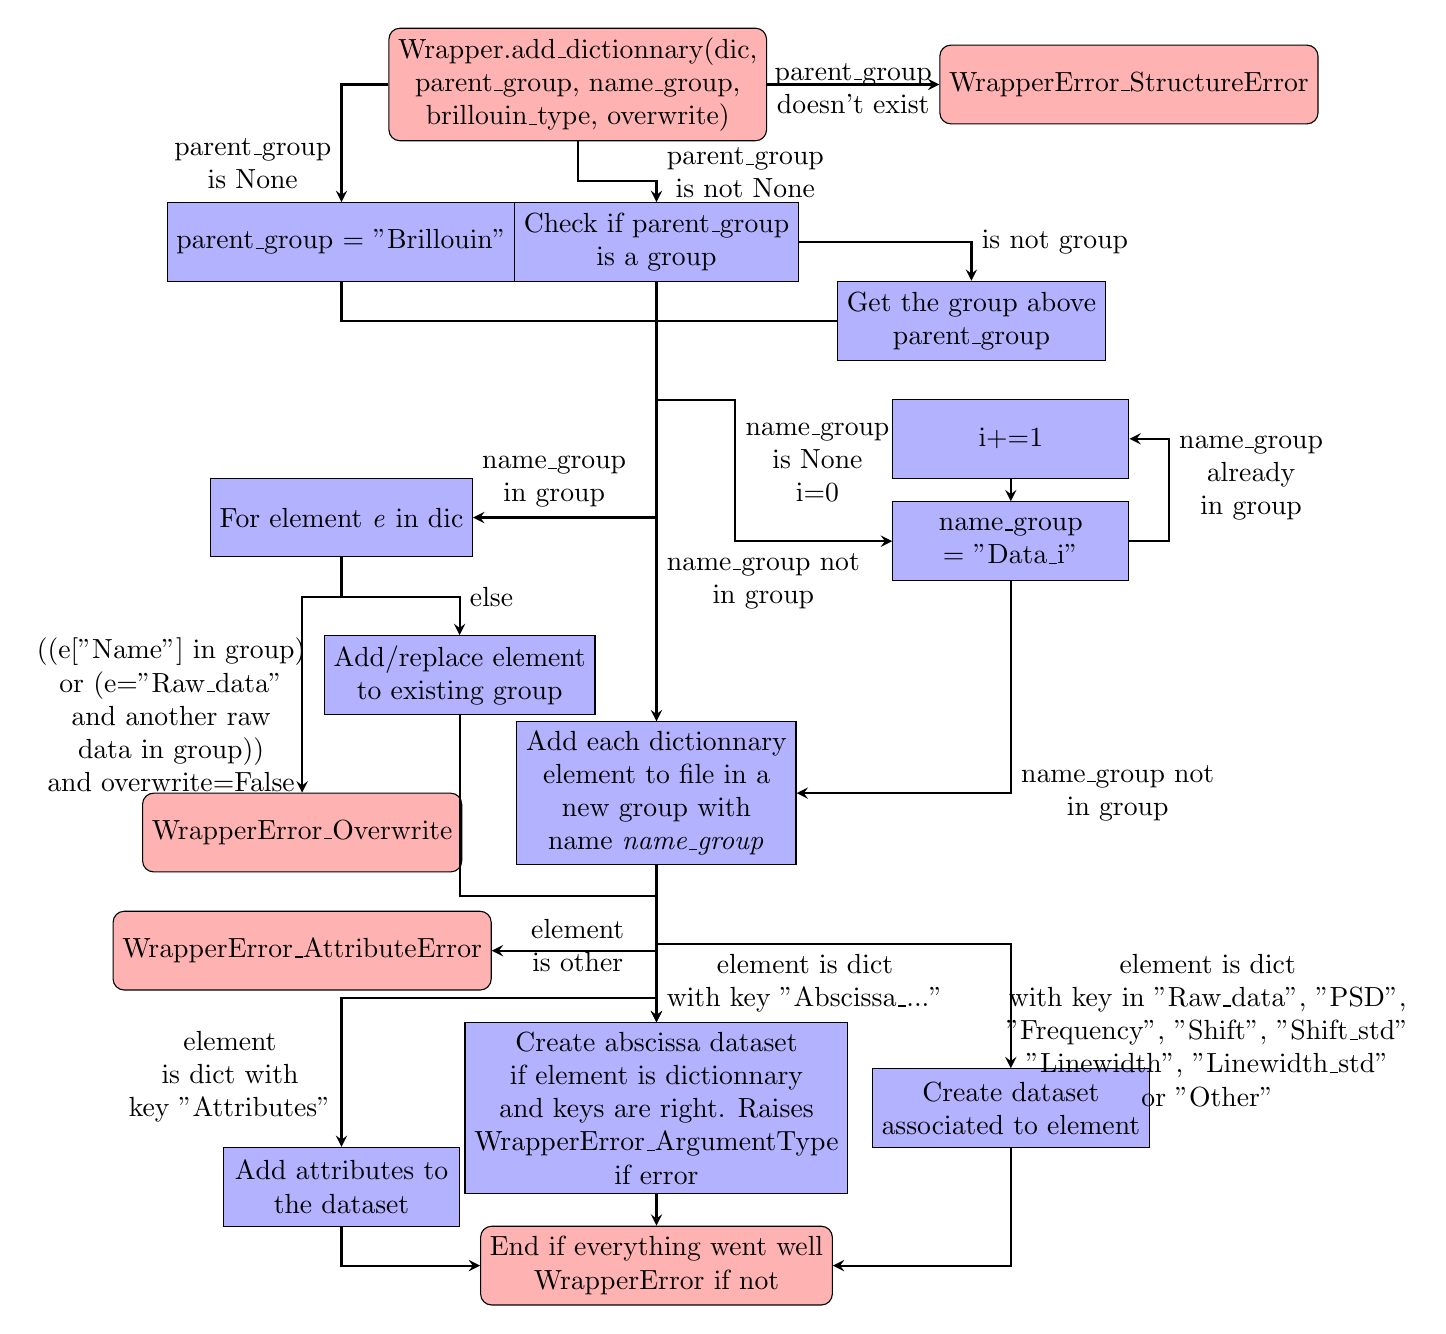
\begin{tikzpicture}[node distance=2cm]
        \node (start) [startstop, align=center] {Wrapper.add\_dictionnary(dic, \\parent\_group, name\_group, \\brillouin\_type, overwrite)};
        \node (setParent) [process, below of=start, yshift=0cm, xshift=-3cm] {parent\_group = "Brillouin"};
        \node (checkExists) [process, right of=setParent, xshift=2cm, align=center] {Check if parent\_group \\exists in file};
        \node (raiseError1) [startstop, right of=start, xshift=5cm] {WrapperError\_StructureError};
        \node (checkGroup) [process, right of=setParent, xshift=2cm, align=center] {Check if parent\_group \\is a group};
        \node (getGroup) [process, right of=checkGroup, yshift=-1cm, xshift = 2cm, align=center] {Get the group above\\ parent\_group};
        \node (name0) [process, below of=checkGroup, yshift=-1.8cm, xshift = 4.5cm, align=center] {name\_group\\ = "Data\_i"};
        \node (raiseError2) [process, above of=name0, yshift=0cm, xshift=0cm, yshift=-0.7cm] {i+=1};
        \node (addData) [process, below of=checkExists, yshift=-5cm, xshift=0cm, align=center] {Add each dictionnary \\ element to file in a\\ new group with \\ name \textit{name\_group}};
        \node (iterateKeys) [process, below of=setParent, yshift=-1.5cm, align=center] {For element \textit{e} in dic};
        \node (nameOverwrite) [process, below of=iterateKeys, yshift=0cm, xshift=1.5cm, align=center] {Add/replace element\\to existing group};
        \node (raiseError3) [startstop, below of=iterateKeys, yshift=-2cm, xshift=-0.5cm, align=center] {WrapperError\_Overwrite};
        \node (addAbscissa) [process, below of=addData, yshift=-2cm, align=center] {Create abscissa dataset\\ if element is dictionnary\\ and keys are right. Raises\\ WrapperError\_ArgumentType \\if error};
        \node (raiseError4) [startstop, left of=addAbscissa, xshift=-2.5cm, yshift=2cm, align=center] {WrapperError\_AttributeError};
        \node (addAttributes) [process, left of=addAbscissa, xshift=-2cm, yshift=-1cm, align=center] {Add attributes to\\ the dataset};
        \node (addNormal) [process, right of=addAbscissa, xshift=2.5cm, align=center] {Create dataset\\associated to element};
        \node (end) [startstop, below of=addAbscissa, align=center] {End if everything went well\\ WrapperError if not};

        \draw [arrow] (start) -| node[anchor=east, align=center, yshift=-1cm] {parent\_group \\is None} (setParent);
        \draw [arrow] ++(start.south) -- +(0mm, -0.5cm) -| node[anchor=west, align=center, xshift=0cm, yshift=0.1cm] {parent\_group \\is not None} (checkGroup.north);
        \draw [arrow] (start) -- node[anchor=north, align=center,yshift=0.4cm] {parent\_group \\doesn't exist} (raiseError1);
        \draw [arrow] ++(checkGroup.south) |- +(0cm,-1.5cm) -| +(1cm,-1.5cm) |- node[anchor=west, yshift=1cm, xshift=0cm, align=center] {name\_group\\ is None\\i=0} (name0.west);
        \draw [arrow] (checkGroup) -| node[anchor=west] {is not group} (getGroup);
        \draw [arrow] (checkGroup) |- node[anchor=south, xshift=-1.3cm, align=center] {name\_group\\ in group}(iterateKeys);
        \draw [arrow] ++(iterateKeys.south) |- +(0cm,-0.5cm) -| node[anchor=west, yshift=-1.5cm, xshift=-3.5cm, align=center] {((e["Name"] in group)\\or (e="Raw\_data" \\ and another raw \\  data in group)) \\and overwrite=False} (raiseError3.north);
        \draw [arrow] ++(iterateKeys.south) |- +(0cm,-0.5cm) -| node[anchor=west, yshift=0cm, xshift=0cm, align=center] {else} (nameOverwrite.north);
        \draw [arrow] (raiseError2.south) -| (name0.north);
        \draw [arrow] ++(name0.east) -| +(0.5cm, 0cm)|- node[anchor=west, align=center, yshift=-0.5cm] {name\_group\\ already\\ in group} (raiseError2.east);
        \draw [arrow] (name0) |- node[anchor=west, align=center, xshift=0cm, yshift=0cm] {name\_group not\\ in group} (addData);
        \draw [arrow] ++(checkGroup.south) |- +(0cm, -2cm) -| node[anchor=west, align=center, yshift=-1.8cm] {name\_group not\\ in group} (addData.north);
        \draw [line] (setParent.south) |- (getGroup.west);
        \draw [arrow] (addData) -- node[anchor=west, align=center, yshift=-0.5cm] {element is dict\\ with key "Abscissa\_..."} (addAbscissa);
        \draw [arrow] ++(addData) |- +(0cm,-2.6cm) -| node[anchor=east, align=center, yshift=-1cm] {element\\ is dict with\\ key "Attributes"} (addAttributes);
        \draw [arrow] ++(addData.south) |- node[anchor=south, align=center, xshift=-1cm, yshift=-0.4cm] {element\\ is other} (raiseError4.east);
        \draw [arrow] ++(nameOverwrite.south)|- +(0cm, -2.3cm) -|  (addAbscissa.north);
        \draw [arrow] ++(addData.south) |- +(0cm, -1cm) -| node[anchor=north, align=center, xshift=2.5cm, yshift=0cm] {element is dict\\ with key in "Raw\_data", "PSD",\\"Frequency", "Shift", "Shift\_std"\\ "Linewidth", "Linewidth\_std" \\ or "Other"} (addNormal.north);
        \draw [arrow] (addAbscissa) -- (end);
        \draw [arrow] (addNormal) |- (end);
        \draw [arrow] (addAttributes) |- (end);
    \end{tikzpicture}
    \caption{Flowchart of the add\_dictionnary method}
\end{figure}


\subsection{Wrapper.add\_dictionary} \label{subchapter:wrapper.add_dictionary}
    This method is the preferred way to add datasets or attributes to the HDF5 file. One or more datasets can be added at once by specifying them as keys of the dictionary to add. Each key is a dictionary composed of at least two keys for datasets: "Data" and "Name". Attributes can also be added to the dataset by adding a key "Attributes" to the dictionary. 
Please refer to \hyperref[chapter:HDF5_BLS.wrapper]{the dedicated section of the tutorial}

\begin{lstlisting}
def add_dictionary(self, dic = None, parent_group = "Brillouin", create_group = False, brillouin_type_parent_group = None, overwrite = False):
\end{lstlisting}

\paragraph*{Attributes:}

\begin{itemize}
    \item \textbf{dic}: The dictionary to add to the wrapper. The keys of the dictionary correspond to the type of data to be added. These keys are identical to the Brillouin\_types for dataset defined in \hyperref[subsec:preamble.file_structure.complete_structure]{preamble}. Each element of the dictionary is another dictionary with the following keys:
    \begin{itemize}
        \item "Name": The name of the dataset that will be stored. This can be any name that the user wants and find useful.
        \item "Data": The array that will be stored, or the dictionary if we are adding attributes
        \item "Units": \textit{Specific to "Abscissa\_..." keys}. The unit of the abscissa
        \item "Dim\_start": \textit{Specific to "Abscissa\_..." keys}. The first dimension to which the abscissa corresponds.
        \item "Dim\_end": \textit{Specific to "Abscissa\_..." keys}. The last dimension (excluded) to which the abscissa corresponds
    \end{itemize}
    \item \textbf{parent\_group}: The parent group where to store the data of the HDF5 file, by default the parent group is the top group "Brillouin". The format of this group should be "Brillouin/Measure/...". 
    \item \textbf{create\_group}: An argument to indicate whether to create the group if it does not exist. If False, the function will raise an error if the group does not exist. Default is False.
    \item \textbf{brillouin\_type\_parent\_group} \textit{(optional, default None)}: The type of the group that will store the elements of the dictionary. The possible values are the ones attributed to groups, defined earlier on in the \hyperref[subsec:preamble.file_structure.complete_structure]{preamble}
    \item \textbf{overwrite} \textit{(optional, default False)}: If True, all the elements of the file with a name corresponding to a name given in the dictionary will be overwritten. Similarly any existing argument will be overwritten and Brillouin type will be redefined. Default is False.
\end{itemize}

Here are typical examples of a dictionary passed as attribute:
\begin{lstlisting}
dic_raw = {
    "Raw_data": {
        "Name": "Raw water spectrum", 
        "Data": np.array([...])}
} # a dictionary with a raw data array straight from the spectrometer - for example if you want to do the whole anylisis process with the library.

dic_treated = {
    "Shift": {
        "Name": "Shift", 
        "Data": np.array([...])}
    "Linewidth": {
        "Name": "Shift", 
        "Data": np.array([...])}
    "Abscissa_x": {
        "Name": "x", 
        "Data": np.array([...]),
        "Unit": "microns",
        "Dim_start": 0,
        "Dim_end": 1}
    "Abscissa_y": {
        "Name": "y", 
        "Data": np.array([...]),
        "Unit": "microns",
        "Dim_start": 1,
        "Dim_end": 2},
    "Attributes": {"MEASURE.Sample": "Water",
                   "SPECTROMETER.Type": "TFP"}
} # a dictionary of measures analyzed by a custom treatment - for example if you have your own data and just want to send them following the library's format.
\end{lstlisting}

\paragraph*{Returns:} Nothing

\paragraph*{Raises:}

\begin{itemize}
    \item \textbf{WrapperError\_StructureError}: Raises an error if the parent group does not exist in the HDF5 file or if the type of group is not logical for the data to be added.
    \item \textbf{WrapperError\_Overwrite}: Raises an error if there is a risk of overwriting the data.
    \item \textbf{WrapperError\_ArgumentType}: Raises an error if arguments given to the function do not match the expected type.
\end{itemize}

\paragraph*{Flowchart:}

The function's logic is represented in the following flowchart:
\begin{figure}[H]
    \centering
    \label{fig:wrapper.flowchart_add_dictionary}
    \small
    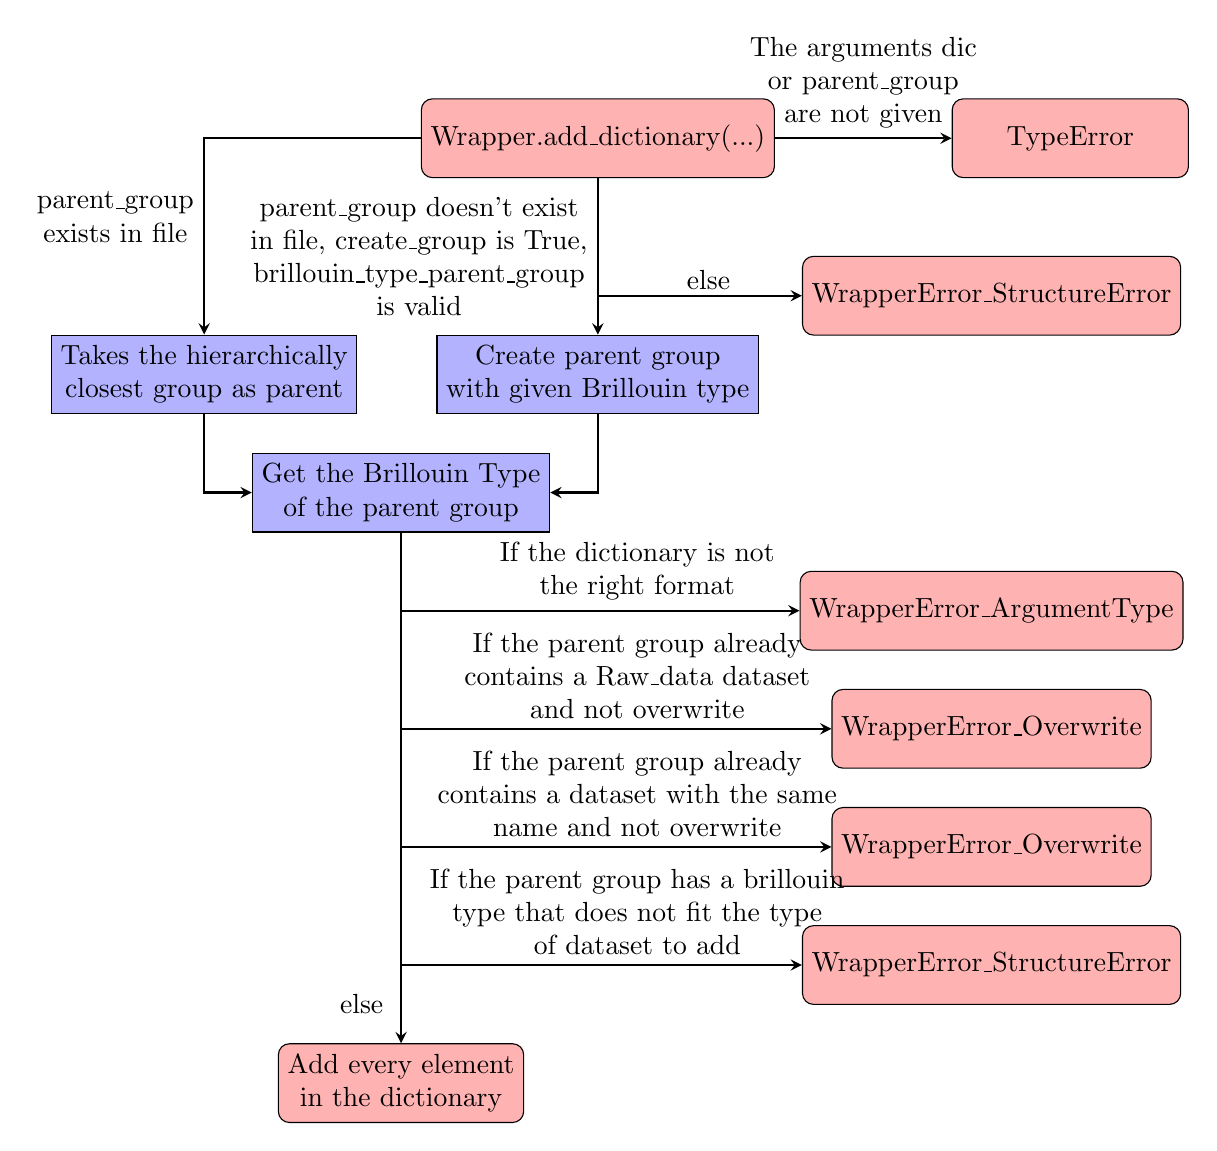
\begin{tikzpicture}[node distance=2cm]
        \node (start) [startstop, align=center] {Wrapper.add\_dictionary(...)};
        \node (error_no_argument) [startstop, right of=start, align = center, yshift=0cm, xshift=4cm] {TypeError};
        \node (take_parent_group) [process, below of=start, align = center, yshift=-1cm, xshift=-5cm] {Takes the hierarchically\\closest group as parent};
        \node (create_parent_group) [process, align=center, below of=start, yshift=-1cm, xshift=0cm] {Create parent group\\with given Brillouin type};
        \node (error_parent_group) [startstop, below of=start, yshift=0cm, xshift=5cm] {WrapperError\_StructureError};
        \node (get_brillouin_type) [process, align=center, below of=take_parent_group, yshift=0.5cm, xshift=2.5cm] {Get the Brillouin Type\\ of the parent group};
        \node (error_dictionary) [startstop, below of=error_parent_group, yshift=-2cm, xshift=0cm] {WrapperError\_ArgumentType};
        \node (error_raw_data) [startstop, below of=error_dictionary, yshift=0.5cm, xshift=0cm] {WrapperError\_Overwrite};
        \node (error_name) [startstop, below of=error_raw_data, yshift=0.5cm, xshift=0cm] {WrapperError\_Overwrite};
        \node (error_parent_type) [startstop, below of=error_name, yshift=0.5cm, xshift=0cm] {WrapperError\_StructureError};
        \node (add_dataset) [startstop, align=center, below of=get_brillouin_type, yshift=-5.5cm, xshift=0cm] {Add every element\\in the dictionary};
 
        \draw [arrow] (start) -| node[anchor=east, align=center, yshift=-1cm] {parent\_group \\exists in file} (take_parent_group);
        \draw [arrow] (start) -- node[anchor=south, align=center, yshift=0cm] {The arguments dic \\or parent\_group \\ are not given} (error_no_argument);
        \draw [arrow] (start) -- node[anchor=east, align=center, yshift=0cm] {parent\_group doesn't exist\\ in file, create\_group is True,\\brillouin\_type\_parent\_group \\is valid} (create_parent_group);
        \draw [arrow] (start) |- node[anchor=west, align=center, yshift=0.2cm, xshift=1cm] {else} (error_parent_group);
        \draw [arrow] (create_parent_group.south) |- node[anchor=west, align=center, yshift=0cm, xshift=0cm] {} (get_brillouin_type);
        \draw [arrow] (take_parent_group.south) |- node[anchor=west, align=center, yshift=0cm, xshift=0cm] {} (get_brillouin_type);
        \draw [arrow] (get_brillouin_type.south) |- node[anchor=south, align=center, yshift=0cm, xshift=3cm] {If the dictionary is not \\the right format} (error_dictionary);
        \draw [arrow] (get_brillouin_type.south) |- node[anchor=south, align=center, yshift=0cm, xshift=3cm] {If the parent group already\\contains a Raw\_data dataset\\and not overwrite} (error_raw_data);
        \draw [arrow] (get_brillouin_type.south) |- node[anchor=south, align=center, yshift=0cm, xshift=3cm] {If the parent group already\\contains a dataset with the same\\name and not overwrite} (error_name);
        \draw [arrow] (get_brillouin_type.south) |- node[anchor=south, align=center, yshift=0cm, xshift=3cm] {If the parent group has a brillouin\\type that does not fit the type\\of dataset to add} (error_parent_type);
        \draw [arrow] (get_brillouin_type.south) -- node[anchor=south, align=center, yshift=-3cm, xshift=-0.5cm] {else} (add_dataset.north);
    \end{tikzpicture}
    \caption{Flowchart of the add\_dictionary method}
\end{figure}


\subsection{Wrapper.create\_group} \label{subchapter:wrapper.create_group}
    This method allows the user to create a new group inside the HDF5 file. This is done by verifying that no overwritting occurs and that the parent group exists.

\begin{lstlisting}
def create_group(self, name, parent_group = None):
\end{lstlisting}

\paragraph{Attributes:}

\begin{itemize}
    \item \textbf{name}: The name of the group to create.
    \item \textbf{parent\_group} \textit{(optional, default None)}: The parent group where to store the data of the HDF5 file, by default the parent group is the top group "Brillouin". The format of this group should be "Brillouin/Measure/...". 
    \item \textbf{brillouin\_type} \textit{(optional, default "Root")}: The type of the group that has been created. By default "Root". The possible values are listed in \hyperref[subsec:preamble.file_structure.complete_structure]{preamble}
    \item \textbf{overwrite} \textit{(optional, default False)}: If True, if a group of the same name already exists in the selected parent group, all its elements will be deleted.
\end{itemize}

\paragraph{Returns:} Nothing

\paragraph{Raises:}

\begin{itemize}
    \item \textbf{WrapperError\_Overwrite}: Raises an error if the group name already exists at the selected parent path.
    \item \textbf{WrapperError\_StructureError}: Raises an error if the parent group does not exist in the HDF5 file.
\end{itemize}

\paragraph{Flowchart:}

The function's logic is represented in the following flowchart:
\begin{figure}[H]
    \centering
    \label{fig:wrapper.flowchart_create_group}
    \small
    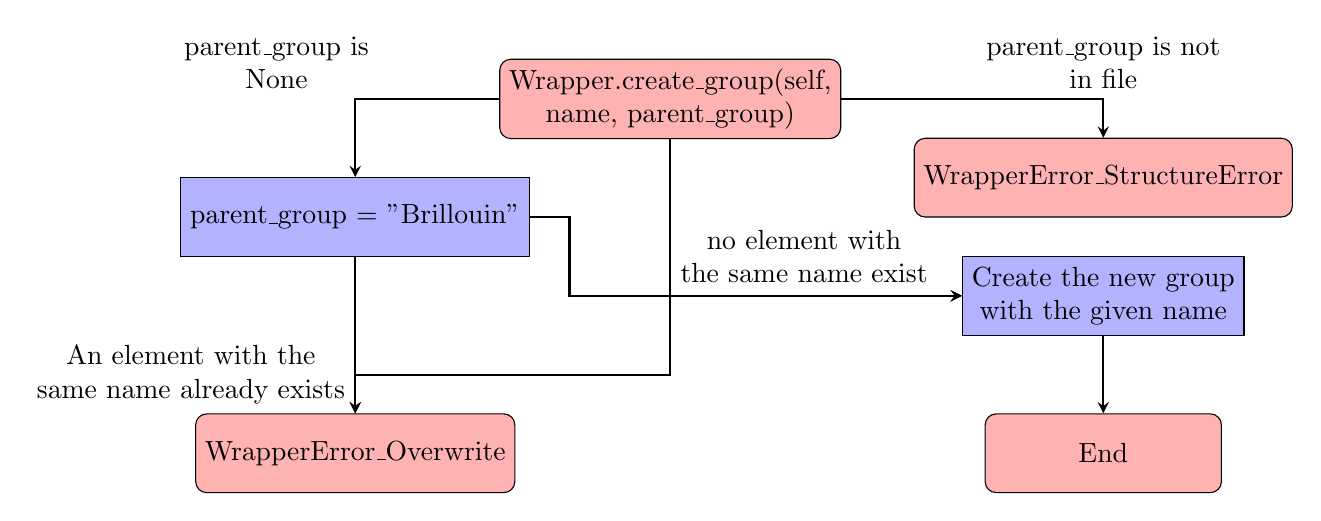
\begin{tikzpicture}[node distance=1cm]
        \node (start) [startstop, xshift=0cm, align=center] {Wrapper.create\_group(self, \\name, parent\_group)};
        \node (setParent) [process, below of=start, yshift=-0.5cm, xshift=-4cm, align=center] {parent\_group = "Brillouin"};
        \node (raiseError1) [startstop, right of=start, xshift=4.5cm, yshift=-1cm] {WrapperError\_StructureError};
        \node (raiseError2) [startstop, below of=setParent, xshift=0cm, yshift=-2cm] {WrapperError\_Overwrite};
        \node (createGroup) [process, below of=raiseError1, yshift=-0.5cm, xshift=0cm, align=center] {Create the new group\\ with the given name};
        \node (end) [startstop, below of=createGroup, xshift=0cm, yshift=-1cm, align=center] {End};

        \draw [arrow] (start) -| node[anchor=south, align=center, yshift=0cm, xshift=-1cm] {parent\_group is\\ None} (setParent);
        \draw [arrow] (start) -| node[anchor=south, align=center, yshift=0cm, xshift=0cm] {parent\_group is not\\ in file} (raiseError1);
        \draw [arrow] (setParent) -- node[anchor=east, align=center, yshift=-0.5cm, xshift=0cm] {An element with the\\ same name already exists} (raiseError2);
        \draw [arrow] (start) |- node[anchor=west, align=center, yshift=0.5cm, xshift=0cm] {no element with\\ the same name exist} (createGroup);
        \draw [arrow] ++(setParent.east) -| +(0.5cm, 0cm) |- (createGroup.west);
        \draw [arrow] ++(start.south) |- +(0cm, -3cm) -| (raiseError2.north);
        \draw [arrow] (createGroup) -- (end);

    \end{tikzpicture}
    \caption{Flowchart of the create\_group method}
\end{figure}

\subsection{Wrapper.delete\_element} \label{subchapter:wrapper.delete_element}
    This method allows the user to delete a dataset or group in the HDF5 file.

\begin{lstlisting}[language=Python]
def delete_element(self, path = None):
\end{lstlisting}

\paragraph{Attributes:}

\begin{itemize}
    \item \textbf{path} \textit{(optional, default None)}: The path to the group or dataset we want to delete in the form "Brillouin/Measure/PSD". If None, the whole file is deleted.
\end{itemize}

\paragraph{Raises:}
\begin{itemize}
    \item \textbf{WrapperError\_StructureError}: If the path does not lead to a valid element in the file.
    \item \textbf{WrapperError}: If there are errors in the deleting process.
\end{itemize}


\paragraph{Flowchart:}

The function's logic is represented in the following flowchart:
\begin{figure}[H]
    \centering
    \label{fig:wrapper.flowchart_delete_element}
    \small
    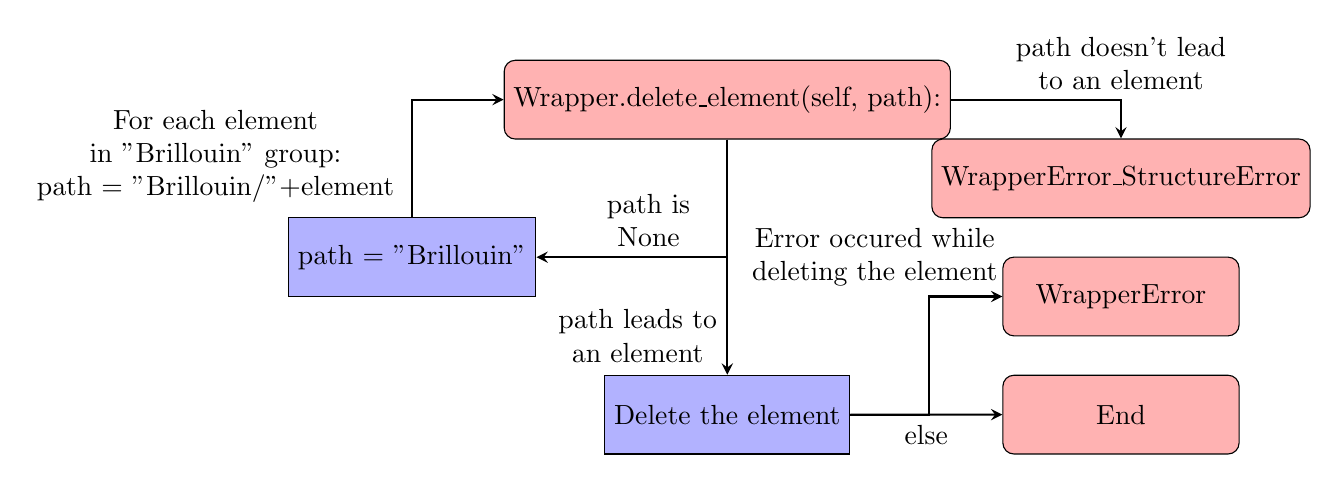
\begin{tikzpicture}[node distance=1cm]
        \node (start) [startstop, xshift=0cm, align=center] {Wrapper.delete\_element(self, path):};
        \node (setPath) [process, below of=start, yshift=-1cm, xshift=-4cm, align=center] {path = "Brillouin"};
        \node (raiseError1) [startstop, right of=start, xshift=4cm, yshift=-1cm] {WrapperError\_StructureError};
        \node (delete) [process, below of=start, yshift=-3cm, xshift=0cm, align=center] {Delete the element};
        \node (raiseError2) [startstop, below of=raiseError1, xshift=0cm, yshift=-0.5cm] {WrapperError};
        \node (end) [startstop, below of=raiseError2, xshift=0cm, yshift=-0.5cm, align=center] {End};

        \draw [arrow] (start) |- node[anchor=south, align=center, yshift=0cm, xshift=-1cm] {path is\\ None} (setPath);
        \draw [arrow] (start) -| node[anchor=south, align=center, yshift=0cm, xshift=0cm] {path doesn't lead\\to an element} (raiseError1);
        \draw [arrow] (setPath) |- node[anchor=north, align=center, yshift=0cm, xshift=-2.5cm] {For each element\\ in "Brillouin" group:\\ path = "Brillouin/"+element} (start);
        \draw [arrow] (start) -- node[anchor=east, align=center, yshift=-1cm, xshift=0cm] {path leads to\\ an element} (delete);
        \draw [arrow] ++(delete.east) -| +(1cm,1cm) |- node[anchor=east, align=center, yshift=0.5cm, xshift=1cm] {Error occured while \\ deleting the element} (raiseError2.west);
        \draw [arrow] (delete) -- node[anchor=north, align=center, yshift=0cm, xshift=0cm] {else} (end);
    \end{tikzpicture}
    \caption{Flowchart of the delete\_element method}
\end{figure}

\subsection{Wrapper.get\_attributes} \label{subchapter:wrapper.get_attributes}
    This method allows the user to extract all the attributes of a dataset or group in a hierarchical way. This means that this method opens the file, goes from the root to the selected group, and extracts all the attributes associated to the groups along the way. The function returns a dictionary, where the keys are the names of the attributes and the values are their values.


\begin{lstlisting}[language=Python]
def get_attributes(self, path = None):
\end{lstlisting}

\paragraph{Attributes:}

\begin{itemize}
    \item \textbf{path} \textit{(optional, default None)}: The path to the group or dataset which attributes we want to extract in the format "Brillouin/Measure/PSD". If None, the attributes of the root group are returned.
\end{itemize}

\paragraph{Returns:} A dictionary containing the attributes of the selected group or dataset where the keys are the names of the attributes and the values are their values. The keys of the attributes are listed in the spreadsheet located in the spreadsheets folder of the project.

\paragraph{Raises:}

\begin{itemize}
    \item \textbf{WrapperError\_StructureError}: Raises an error if the path does not lead to a valid element in the file.
\end{itemize}

\paragraph{Flowchart:}

The function's logic is represented in the following flowchart:
\begin{figure}[H]
    \centering
    \label{fig:wrapper.flowchart_get_attributes}
    \small
    \begin{tikzpicture}[node distance=2cm]
        \node (start) [startstop] {Wrapper.get\_attributes(path=None)};
        \node (setPath) [process, below of=start, yshift=0cm, xshift=-3cm] {path = "Brillouin"};
        \node (extract) [process, right of=setPath, xshift=2cm, align=center] {Extracts attributes \\hierarchically};
        \node (raiseError1) [startstop, right of=checkExists, xshift=3cm] {WrapperError\_StructureError};
        \node (end) [startstop, below of=checkGroup, align=center] {Returns a dictionary\\ of attributes};

        \draw [arrow] (start) -| node[anchor=east, align=center, yshift=-1cm] {path \\is None} (setParent);
        \draw [arrow] (setPath) -- (extract);
        \draw [arrow] ++(start.south) |- +(0cm, -0.5cm) -| node[anchor=west, align=center, yshift=0cm] {path exists} (extract.north);
        \draw [arrow] (start) -| node[anchor=west, align=center] {path does \\not exist} (raiseError1);
        \draw [arrow] (extract) -- (end);
    \end{tikzpicture}
    \caption{Flowchart of the get\_attributes method}
\end{figure}
    

\subsection{Wrapper.get\_structure} \label{subchapter:wrapper.get_structure}
    This method allows the user to extract the structure in the form of a dictionnary. This dictionnary is composed of all the elements of the file and their "Brillouin\_type" attribute, in the form of a JSON file or dictionnary similar to this one:
\begin{verbatim}
{'Brillouin': {'Brillouin_type': 'Root', 
    'M1': {'Brillouin_type': 'Root', 
        'Measure': {'Brillouin_type': 'Measure', 
            'Raw_data': {'Brillouin_type': 'Raw_data'}
            }
        }
    }
}
\end{verbatim}

\begin{lstlisting}[language=Python]
def get_structure(self, filepath = None):
\end{lstlisting}

\paragraph{Attributes:}

\begin{itemize}
    \item \textbf{filepath} \textit{(optional, default None)}: The filepath to a HDF5 file. If None, the file of the wrapper is used.
\end{itemize}

\paragraph{Returns:} A dictionnary representing the structure of the file as detailed \hyperref[subsec:preamble.file_structure.complete_structure]{before}

\paragraph{Flowchart:}

The function's logic is represented in the following flowchart:
\begin{figure}[H]
    \centering
    \label{fig:wrapper.flowchart_get_structure}
    \small
    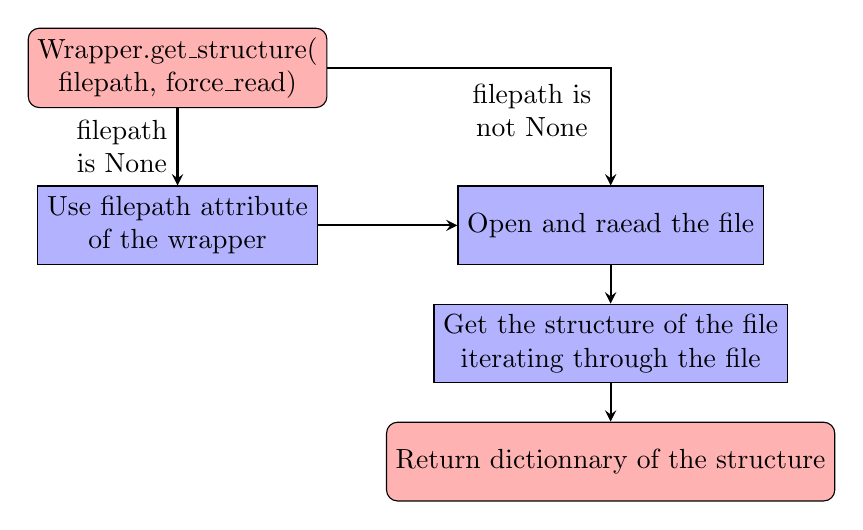
\begin{tikzpicture}[node distance=1.5cm]
        \node (start) [startstop, align=center] {Wrapper.get\_structure(\\filepath, force\_read)};
        \node (setPath) [process, below of=start, yshift=-0.5cm, xshift=0cm, align=center] {Use filepath attribute \\ of the wrapper};
        \node (readFile) [process, right of=setPath, yshift=0cm, xshift=4cm, align=center] {Open and raead the file};
        \node (iterativeStructure) [process, below of=readFile, yshift=0cm, xshift=0cm, align=center] {Get the structure of the file\\ iterating through the file};
        \node (end) [startstop, below of=iterativeStructure, yshift=0cm, xshift=0cm, align=center] {Return dictionnary of the structure};

        \draw [arrow] (start) -- node[anchor=east, align=center, yshift=0cm] {filepath \\is None} (setPath);
        \draw [arrow] (setPath) -- (readFile);
        \draw [arrow] (start) -| node[anchor=south, align=center, xshift=-1cm, yshift=-1cm] {filepath is\\not None} (readFile);
        \draw [arrow] (readFile) -- (iterativeStructure);
        \draw [arrow] ++(iterativeStructure.south) -- (end.north);
    \end{tikzpicture}
    \caption{Flowchart of the get\_structure method}
\end{figure}   

\subsection{Wrapper.save\_as\_hdf5} \label{subchapter:wrapper.save_as_hdf5}
    This method allows the user to save the file to a specified location.

\begin{lstlisting}[language=Python]
def save_as_hdf5(self, filepath = None, remove_old_file = True):
\end{lstlisting}

\paragraph{Attributes:}

\begin{itemize}
    \item \textbf{filepath} \textit{(optional, default None)}: The filepath to the HDF5 file to save to.
    \item \textbf{remove\_old\_file} \textit{(optional, default True)}: A boolean that indicates whether the old file should be removed or not.
\end{itemize}

\paragraph{Raises:}
\begin{itemize}
    \item \textbf{WrapperError\_Overwrite}: If the file already exists.
    \item \textbf{WrapperError}: If an error occured while saving the file.
\end{itemize}


\paragraph{Flowchart:}

The function's logic is represented in the following flowchart:
\begin{figure}[H]
    \centering
    \label{fig:wrapper.flowchart_save_as_hdf5}
    \small
    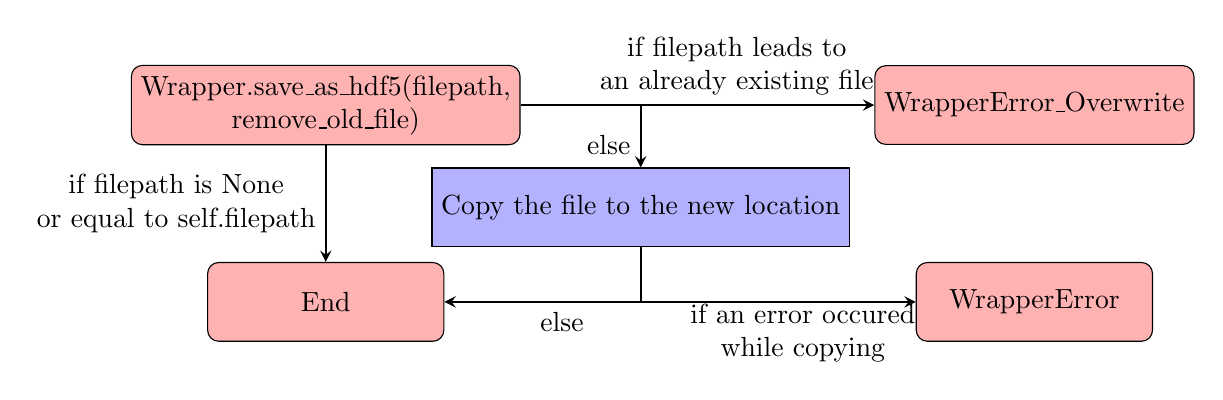
\begin{tikzpicture}[node distance=2cm]
        \node (start) [startstop, xshift=0cm, align=center] {Wrapper.save\_as\_hdf5(filepath, \\remove\_old\_file)};
        \node (raiseError1) [startstop, right of=start, yshift=0cm, xshift=7cm, align=center] {WrapperError\_Overwrite};
        \node (copyFile) [process, below of=start, yshift=0.7cm, xshift=4cm, align=center] {Copy the file to the new location};
        \node (end) [startstop, below of=start, yshift=-0.5cm, xshift=0cm, align=center] {End};
        \node (raiseError2) [startstop, right of=end, yshift=0cm, xshift=7cm, align=center] {WrapperError};

        \draw [arrow] (start) -- node[anchor=east, align=center, yshift=-0cm] {if filepath is None\\ or equal to self.filepath} (end);
        \draw [arrow] (start) -- node[anchor=south, align=center, yshift=-0cm, xshift=0.5cm] {if filepath leads to \\an already existing file} (raiseError1);
        \draw [arrow] (start) -| node[anchor=east, align=center, yshift=-0.5cm, xshift=-0cm] {else} (copyFile);
        \draw [arrow] (copyFile) |- node[anchor=north, align=center, yshift=-0cm, xshift=-1cm] {else} (end);
        \draw [arrow] (copyFile) |- node[anchor=west, align=center, yshift=-0.4cm, xshift=0.5cm] {if an error occured\\ while copying} (raiseError2);
    \end{tikzpicture}
    \caption{Flowchart of the save\_as\_hdf5 method}
\end{figure}

\subsection{Wrapper.set\_attributes\_data} \label{subchapter:wrapper.set_attributes_data}
    This method allows the user to update the attributes of the wrapper with the values of a dictionary. This is the preferred way to update the attributes of a group or dataset of the HDF5 file.

\begin{lstlisting}[language=Python]
def set_attributes_data(self, properties, path = None, overwrite = False):
\end{lstlisting}

\paragraph{Attributes:}

\begin{itemize}
    \item \textbf{properties}: A dicitonnary of the property(ies) to be updated.
    \item \textbf{path} \textit{(optional, default None)}: The path to the group or dataset whose metadata we want to update. If None, the metadata of the root group are updated.
    \item \textbf{overwrite} \textit{(optional, default False)}: If True, the attributes of the selected group or dataset are overwritten. If False, only new attributes are added to the existing ones.
\end{itemize}

\paragraph{Raises:}
\begin{itemize}
    \item \textbf{WrapperError}: If an error occured while updating the metadata in the HDF5 file
\end{itemize}


\paragraph{Flowchart:}

The function's logic is represented in the following flowchart:
\begin{figure}[H]
    \centering
    \label{fig:wrapper.flowchart_set_attributes_data}
    \small
    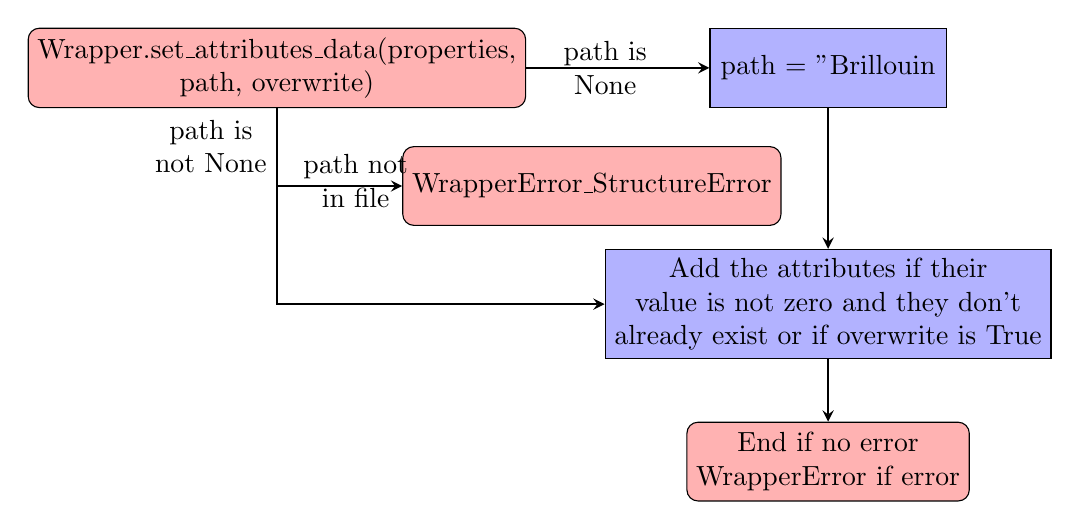
\begin{tikzpicture}[node distance=2cm]
        \node (start) [startstop, xshift=0cm, align=center] {Wrapper.set\_attributes\_data(properties, \\path, overwrite)};
        \node (setPath) [process, right of=start, yshift=0cm, xshift=5cm, align=center] {path = "Brillouin};
        \node (errorPath) [startstop, below of=setPath, yshift=0.5cm, xshift=-3cm, align=center] {WrapperError\_StructureError};
        \node (addMetadata) [process, below of=setPath, yshift=-1cm, xshift=0cm, align=center] {Add the attributes if their \\value is not zero and they don't\\ already exist or if overwrite is True};
        \node (end) [startstop, below of=addMetadata, yshift=0cm, xshift=0cm, align=center] {End if no error\\WrapperError if error};

        \draw [arrow] (start) -- node[anchor=east, align=center, yshift=0cm, xshift=0.5cm] {path is\\ None} (setPath);
        \draw [arrow] (start) |- node[anchor=east, align=center, yshift=2cm] {path is \\not None} (addMetadata);
        \draw [arrow] (start) |- node[anchor=south, align=center, xshift=1cm, yshift=-0.4cm] {path not\\in file} (errorPath.west);
        \draw [arrow] (setPath) -- (addMetadata);
        \draw [arrow] (addMetadata) -- (end);
    \end{tikzpicture}
    \caption{Flowchart of the set\_attributes\_data method}
\end{figure}


        \section{Derived methods of the Wrapper class}
            \subsection{Wrapper.add\_abscissa}\label{subsec:wrapper.add_abscissa}
This method allows the user to add an abscissa to the HDF5 file. It adds the data by calling the \hyperref[subsec:wrapper.add_dictionnary]{Wrapper.add\_dictionnary} method.

\begin{lstlisting}[language=Python]
def add_abscissa(self, data, parent_group=None, name=None, unit = "1" , dim_start = 0, dim_end = None, overwrite = False):
\end{lstlisting}

\paragraph{Attributes:}

\begin{itemize}
    \item \textbf{data}: The abscissa array to add to the wrapper. 
    \item \textbf{parent\_group}: The path to the group or dataset whose the raw data will be added in the form "Brillouin/Measure/...".
    \item \textbf{name} \textit{(optional, default None)}: The name that will be given to the dataset. If None, the name is set to "Raw data".
    \item \textbf{unit} \textit{(optional, default "1")}: The unit of the abscissa (e.g. "microns").
    \item \textbf{dim\_start} \textit{(optional, default 0)}: The first dimension of the abscissa.
    \item \textbf{dim\_end} \textit{(optional, default None)}: The last dimension of the abscissa. If None, the abscissa is considered to be a vector.
    \item \textbf{overwrite} \textit{(optional, default False)}: If True, the attributes of the selected group or dataset are overwritten if they exist in the file.
\end{itemize}

\paragraph{Raises:}
\begin{itemize}
    \item All the errors of the \hyperref[subsec:wrapper.add_dictionnary]{Wrapper.add\_dictionnary} method.
\end{itemize}


\subsection{Wrapper.add\_frequency}\label{subsec:wrapper.add_frequency}
This method allows the user to add a frequency array to the HDF5 file. It adds the data by calling the \hyperref[subchapter:wrapper.add_dictionary]{Wrapper.add\_dictionary} method.
By default, the frequency array is stored in "GHz". Note however that this will just affect the presentation of the results and not the process itself.

\begin{lstlisting}[language=Python]
def add_frequency(self, data, parent_group, name = None, overwrite = False):
\end{lstlisting}

\paragraph{Attributes:}

\begin{itemize}
    \item \textbf{data}: The frequency array to add to the wrapper. 
    \item \textbf{parent\_group}: The path to the group or dataset where the frequency will be added in the form "Brillouin/Measure/...".
    \item \textbf{name} \textit{(optional, default None)}: The name that will be given to the dataset. If None, the name is set to "Frequency".
    \item \textbf{overwrite} \textit{(optional, default False)}: If True, the attributes of the selected group or dataset are overwritten if they exist in the file.
\end{itemize}

\paragraph{Raises:}
\begin{itemize}
    \item \textbf{WrapperError\_StructureError}: If the parent group does not exist in the HDF5 file.
    \item All the errors of the \hyperref[subchapter:wrapper.add_dictionary]{Wrapper.add\_dictionary} method.
\end{itemize}


\subsection{Wrapper.add\_PSD}\label{subsec:wrapper.add_psd}
This method allows the user to add a Power Spectral Density array to the HDF5 file. It adds the data by calling the \hyperref[subchapter:wrapper.add_dictionary]{Wrapper.add\_dictionary} method.

\begin{lstlisting}[language=Python]
def add_PSD(self, data, parent_group, name = None, overwrite = False):
\end{lstlisting}

\paragraph{Attributes:}

\begin{itemize}
    \item \textbf{data}: The PSD array to add to the wrapper. 
    \item \textbf{parent\_group}: The path to the group or dataset where the frequency will be added in the form "Brillouin/Measure/...".
    \item \textbf{name} \textit{(optional, default None)}: The name that will be given to the dataset. If None, the name is set to "PSD".
    \item \textbf{overwrite} \textit{(optional, default False)}: If True, the attributes of the selected group or dataset are overwritten if they exist in the file.
\end{itemize}

\paragraph{Raises:}
\begin{itemize}
    \item \textbf{WrapperError\_StructureError}: If the parent group does not exist in the HDF5 file.
    \item All the errors of the \hyperref[subchapter:wrapper.add_dictionary]{Wrapper.add\_dictionary} method.
\end{itemize}


\subsection{Wrapper.add\_raw\_data}\label{subsec:wrapper.add_raw_data}
This method allows the user to add raw data to the HDF5 file. It adds the data by calling the \hyperref[subsec:wrapper.add_dictionnary]{Wrapper.add\_dictionnary} method.

\begin{lstlisting}[language=Python]
def add_raw_data(self, data, parent_group, name = None, overwrite = False):
\end{lstlisting}

\paragraph{Attributes:}

\begin{itemize}
    \item \textbf{data}: The data to add to the wrapper. 
    \item \textbf{parent\_group}: The path to the group or dataset whose the raw data will be added in the form "Brillouin/Measure/...".
    \item \textbf{name} \textit{(optional, default None)}: The name that will be given to the dataset. If None, the name is set to "Raw data".
    \item \textbf{overwrite} \textit{(optional, default False)}: If True, the attributes of the selected group or dataset are overwritten if they exist in the file.
\end{itemize}

\paragraph{Raises:}
\begin{itemize}
    \item \textbf{WrapperError\_StructureError}: If the parent group does not exist in the HDF5 file.
    \item All the errors of the \hyperref[subsec:wrapper.add_dictionnary]{Wrapper.add\_dictionnary} method.
\end{itemize}


\subsection{Wrapper.add\_treated\_data}\label{subsec:wrapper.add_treated_data}
This method allows the user to add the result of a treatment to the HDF5 file. It adds the data by calling the \hyperref[subsec:wrapper.add_dictionnary]{Wrapper.add\_dictionnary} method.

\begin{lstlisting}[language=Python]
def add_treated_data(self, shift, linewidth, shift_std, linewidth_std, parent_group, name_group = None, overwrite = False):
\end{lstlisting}

\paragraph{Attributes:}

\begin{itemize}
    \item \textbf{shift}: The shift array to add to the wrapper. 
    \item \textbf{linewidth}: The linewidth array to add to the wrapper. 
    \item \textbf{shift\_std}: The standard deviation of the shift array to add to the wrapper. 
    \item \textbf{linewidth\_std}: The standard deviation of the linewidth array to add to the wrapper. 
    \item \textbf{parent\_group}: The path to the group or dataset whose the raw data will be added in the form "Brillouin/Measure/...".
    \item \textbf{name\_group} \textit{(optional, default None)}: The name that will be given to the group containing all the treated dataset. If None, the name is set to "Treat\_i" where "i" is an integer that ensures that the name is unique.
    \item \textbf{overwrite} \textit{(optional, default False)}: If True, the attributes of the selected group or dataset are overwritten if they exist in the file.
\end{itemize}

\paragraph{Raises:}
\begin{itemize}
    \item \textbf{WrapperError\_StructureError}: If the parent group does not exist in the HDF5 file.
    \item All the errors of the \hyperref[subsec:wrapper.add_dictionnary]{Wrapper.add\_dictionnary} method.
\end{itemize}


\subsection{Wrapper.import\_abscissa}\label{subsec:wrapper.import_abscissa}
This method allows the user to add an abscissa to the HDF5 file from a measure file. It adds the data by calling the \hyperref[subchapter:wrapper.add_abscissa]{Wrapper.add\_abscissa} method.

\begin{lstlisting}[language=Python]
def add_abscissa(self, filepath, parent_group, creator = None, parameters = None, name=None, unit = "AU" , dim_start = 0, dim_end = None, reshape = None, overwrite = False):
\end{lstlisting}

\paragraph{Attributes:}

\begin{itemize}
    \item \textbf{filepath}: The path to the file containing the abscissa to import.
    \item \textbf{parent\_group}: The path to the group or dataset whose the raw data will be added in the form "Brillouin/Measure/...".
    \item \textbf{creator} \textit{(optional, default None)}: The structure of the file that has to be loaded. If None, a LoadError can be raised.
    \item \textbf{parameters} \textit{(optional, default None)}: The parameters that are to be used to import the data correctly.  If None, a LoadError can be raised.
    \item \textbf{name} \textit{(optional, default None)}: The name that will be given to the dataset. If None, the name is set to "Raw data".
    \item \textbf{unit} \textit{(optional, default "1")}: The unit of the abscissa (e.g. "microns").
    \item \textbf{dim\_start} \textit{(optional, default 0)}: The first dimension of the abscissa.
    \item \textbf{dim\_end} \textit{(optional, default None)}: The last dimension of the abscissa. If None, the abscissa is considered to be a vector.
    \item \textbf{reshape} \textit{(optional, default None)}: The new shape of the array. If None, the shape is not changed.
    \item \textbf{overwrite} \textit{(optional, default False)}: If True, the attributes of the selected group or dataset are overwritten if they exist in the file.
\end{itemize}

\paragraph{Raises:}
\begin{itemize}
    \item \textbf{WrapperError\_FileNotFound}: If the file could not be found.  
    \item All the errors of the \hyperref[subchapter:wrapper.add_abscissa]{Wrapper.add\_abscissa} method.
    \item All the LoadError errors of the load\_data module.
\end{itemize}


\subsection{Wrapper.import\_frequency}\label{subsec:wrapper.import_frequency}
This method allows the user to import a frequency array to the HDF5 file. It adds the data by calling the \hyperref[subsec:wrapper.add_frequency]{Wrapper.add\_frequency} method.
By default, the frequency array is stored in "GHz". Note however that this will just affect the presentation of the results and not the process itself.

\begin{lstlisting}[language=Python]
def import_frequency(self, filepath, parent_group, creator = None, parameters = None, name = None, reshape = None, overwrite = False):
\end{lstlisting}

\paragraph{Attributes:}

\begin{itemize}
    \item \textbf{filepath}: The frequency array to add to the wrapper. 
    \item \textbf{parent\_group}: The path to the group or dataset where the frequency will be added in the form "Brillouin/Measure/...".
    \item \textbf{creator} \textit{(optional, default None)}: The structure of the file that has to be loaded. If None, a LoadError can be raised.
    \item \textbf{parameters} \textit{(optional, default None)}: The parameters that are to be used to import the data correctly.  If None, a LoadError can be raised.
    \item \textbf{name} \textit{(optional, default None)}: The name that will be given to the dataset. If None, the name is set to "Frequency".
    \item \textbf{reshape} \textit{(optional, default None)}: The new shape of the array. If None, the shape is not changed.
    \item \textbf{overwrite} \textit{(optional, default False)}: If True, the attributes of the selected group or dataset are overwritten if they exist in the file.
\end{itemize}

\paragraph{Raises:}
\begin{itemize}
    \item \textbf{WrapperError\_FileNotFound}: If the file could not be found.
    \item All the errors of the \hyperref[subsec:wrapper.add_frequency]{Wrapper.add\_frequency} method.
    \item All the LoadError errors of the load\_data module.
\end{itemize}


\subsection{Wrapper.import\_PSD}\label{subsec:wrapper.import_psd}
This method allows the user to import raw data to the HDF5 file. It adds the data by calling the \hyperref[subchapter:wrapper.add_raw_data]{Wrapper.add\_raw\_data} method.


\begin{lstlisting}[language=Python]
def import_raw_data(self, filepath, parent_group, creator = None, parameters = None, name = None, reshape = None, overwrite = False):
\end{lstlisting}

\paragraph{Attributes:}

\begin{itemize}
    \item \textbf{filepath}: The filepath to the raw data to import.
    \item \textbf{parent\_group}: The path to the group or dataset where the frequency will be added in the form "Brillouin/Measure/...".
    \item \textbf{creator} \textit{(optional, default None)}: The structure of the file that has to be loaded. If None, a LoadError can be raised.
    \item \textbf{parameters} \textit{(optional, default None)}: The parameters that are to be used to import the data correctly.  If None, a LoadError can be raised.
    \item \textbf{name} \textit{(optional, default None)}: The name that will be given to the dataset. If None, the name is set to "Frequency".
    \item \textbf{reshape} \textit{(optional, default None)}: The new shape of the array. If None, the shape is not changed.
    \item \textbf{overwrite} \textit{(optional, default False)}: If True, the attributes of the selected group or dataset are overwritten if they exist in the file.
\end{itemize}

\paragraph{Raises:}
\begin{itemize}
    \item \textbf{WrapperError\_FileNotFound}: If the file could not be found.
    \item All the errors of the \hyperref[subchapter:wrapper.add_frequency]{Wrapper.add\_frequency} method.
    \item All the LoadError errors of the load\_data module.
\end{itemize}


\subsection{Wrapper.import\_raw\_data}\label{subsec:wrapper.import_raw_data}
This method allows the user to add a Power Spectral Density array to the HDF5 file from a file. It adds the data by calling the \hyperref[subchapter:wrapper.add_psd]{Wrapper.add\_PSD} method.


\begin{lstlisting}[language=Python]
def import_PSD(self, filepath, parent_group, creator = None, parameters = None, name = None, reshape = None, overwrite = False):
\end{lstlisting}

\paragraph{Attributes:}

\begin{itemize}
    \item \textbf{filepath}: The path to the file containing the PSD to import.
    \item \textbf{parent\_group}: The path to the group or dataset where the frequency will be added in the form "Brillouin/Measure/...".
    \item \textbf{creator} \textit{(optional, default None)}: The structure of the file that has to be loaded. If None, a LoadError can be raised.
    \item \textbf{parameters} \textit{(optional, default None)}: The parameters that are to be used to import the data correctly.  If None, a LoadError can be raised.
    \item \textbf{name} \textit{(optional, default None)}: The name that will be given to the dataset. If None, the name is set to "PSD".
    \item \textbf{reshape} \textit{(optional, default None)}: The new shape of the array. If None, the shape is not changed.
    \item \textbf{overwrite} \textit{(optional, default False)}: If True, the attributes of the selected group or dataset are overwritten if they exist in the file.
\end{itemize}


\paragraph{Raises:}
\begin{itemize}
    \item \textbf{WrapperError\_FileNotFound}: If the file could not be found.
    \item All the errors of the \hyperref[subchapter:wrapper.add_psd]{Wrapper.add\_PSD} method.
    \item All the LoadError errors of the load\_data module.
\end{itemize}

\subsection{Wrapper.import\_treated\_data}\label{subsec:wrapper.import_treated_data}
This method allows the user to import the arrays resulting from a treatment to the HDF5 file. It adds the data by calling the \hyperref[subchapter:wrapper.add_psd]{Wrapper.add\_PSD} method.


\begin{lstlisting}[language=Python]
def import_treated_data(self, filepath_shift, filepath_linewidth, filepath_shift_err, filepath_linewidth_err, parent_group, creator = None, parameters = None, name = None, reshape = None, overwrite = False):
\end{lstlisting}

\paragraph{Attributes:}

\begin{itemize}
    \item \textbf{filepath\_shift}: The path to the file containing the shift array to import.
    \item \textbf{filepath\_linewidth}: The path to the file containing the linewidth array to import.
    \item \textbf{filepath\_shift\_err}: The path to the file containing the shift error array to import.
    \item \textbf{filepath\_linewidth\_err}: The path to the file containing the linewidth error array to import.
    \item \textbf{parent\_group}: The path to the group or dataset where the frequency will be added in the form "Brillouin/Measure/...".
    \item \textbf{creator} \textit{(optional, default None)}: The structure of the files that have to be loaded. If None, a LoadError can be raised.
    \item \textbf{parameters} \textit{(optional, default None)}: The parameters that are to be used to import the data correctly.  If None, a LoadError can be raised.
    \item \textbf{name} \textit{(optional, default None)}: The name that will be given to the dataset. If None, the name is set to "PSD".
    \item \textbf{reshape} \textit{(optional, default None)}: The new shape of the array. If None, the shape is not changed.
    \item \textbf{overwrite} \textit{(optional, default False)}: If True, the attributes of the selected group or dataset are overwritten if they exist in the file.
\end{itemize}


\paragraph{Raises:}
\begin{itemize}
    \item \textbf{WrapperError\_FileNotFound}: If one of the files could not be found.
    \item All the errors of the \hyperref[subchapter:wrapper.add_treated_data]{Wrapper.add\_treated\_data} method.
    \item All the LoadError errors of the load\_data module.
\end{itemize}





\subsection{Wrapper.import\_properties\_data}\label{subsec:wrapper.import_properties_data}
This method allows the user to import data from a CSV, XLS or XLSX file to a dataset or group of the HDF5 file. It reads the data from the file and updates the metadata by calling the \hyperref[subchapter:wrapper.set_attributes_data]{Wrapper.set\_attributes\_data} method.

\begin{lstlisting}[language=Python]
def import_properties_data(self, filepath, path = None, overwrite = False):
\end{lstlisting}

\paragraph{Attributes:}

\begin{itemize}
    \item \textbf{filepath}: The filepath to the file containing the updated properties.
    \item \textbf{path} \textit{(optional, default None)}: The path to the group or dataset whose metadata we want to update in the form: "Brillouin/Measure". If None, the metadata of the root group are updated.
    \item \textbf{overwrite} \textit{(optional, default False)}: If True, the attributes of the selected group or dataset are overwritten. If False, only new attributes are added to the existing ones.
\end{itemize}

\paragraph{Raises:}
\begin{itemize}
    \item \textbf{WrapperError\_FileNotFound}: If the file with the properties is not found or not valid.
    \item All the errors of the \hyperref[subchapter:wrapper.set_attributes_data]{Wrapper.set\_attributes\_data} method.
\end{itemize}


\paragraph{Flowchart:}

The function's logic is represented in the following flowchart:
\begin{figure}[H]
    \centering
    \label{fig:wrapper.flowchart_import_properties_data}
    \small
    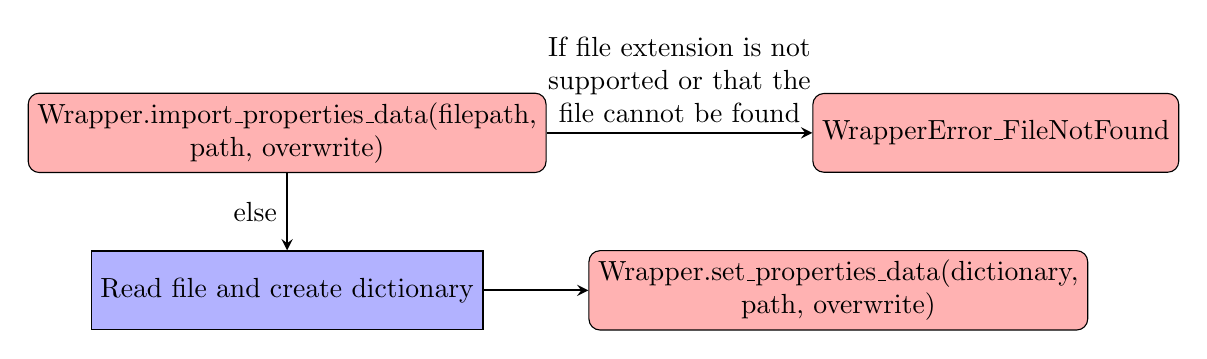
\begin{tikzpicture}[node distance=2cm]
        \node (start) [startstop, xshift=0cm, align=center] {Wrapper.import\_properties\_data(filepath, \\path, overwrite)};
        \node (fileError) [startstop, right of=start, xshift=7cm, align=center] {WrapperError\_FileNotFound};
        \node (readFile) [process, below of=start] {Read file and create dictionary};
        \node (setProperties) [startstop, right of=readFile, xshift=5cm, align=center] {Wrapper.set\_properties\_data(dictionary, \\path, overwrite)};

        \draw [arrow] (start) -- node[anchor=south, align=center, yshift=0cm, xshift=0cm] {If file extension is not\\ supported or that the \\file cannot be found} (fileError);
        \draw [arrow] (start) -- node[anchor=east, align=center, yshift=0cm, xshift=0cm] {else} (readFile);
        \draw [arrow] (readFile) -- (setProperties);
    \end{tikzpicture}
    \caption{Flowchart of the import\_properties\_data method}
\end{figure}

\subsection{Wrapper.update\_property}\label{subsec:wrapper.update_property}
This method allows the user to update one attribute of the wrapper. This method is based on the \hyperref[subchapter:wrapper.set_attributes_data]{Wrapper.set\_attributes\_data} method.

\begin{lstlisting}[language=Python]
def update_property(self, name, value, path = None):
\end{lstlisting}

\paragraph{Attributes:}

\begin{itemize}
    \item \textbf{name}: The name of the attribute to update.
    \item \textbf{value}: The new value of the attribute.
    \item \textbf{path} \textit{(optional, default None)}: The path to the group or dataset whose metadata we want to update in the form: "Brillouin/Measure". If None, the metadata of the root group are updated.
\end{itemize}

\paragraph{Raises:}
\begin{itemize}
    \item All the errors of the \hyperref[subchapter:wrapper.set_attributes_data]{Wrapper.set\_attributes\_data} method.
\end{itemize}


\paragraph{Flowchart:}

The function's logic is represented in the following flowchart:
\begin{figure}[H]
    \centering
    \label{fig:wrapper.flowchart_update_property}
    \small
    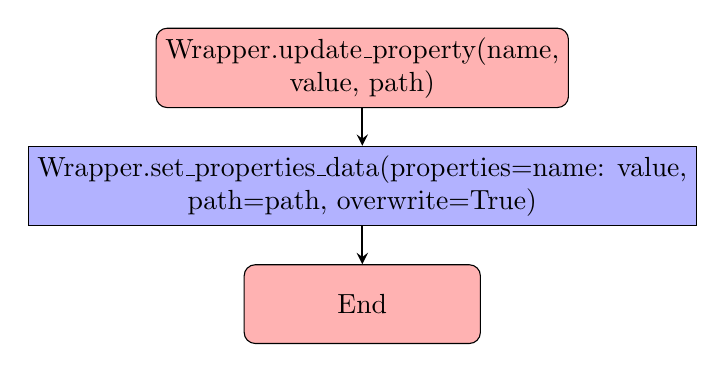
\begin{tikzpicture}[node distance=1.5cm]
        \node (start) [startstop, xshift=0cm, align=center] {Wrapper.update\_property(name, \\value, path)};
        \node (setProperty) [process, below of=start, align=center] {Wrapper.set\_properties\_data(properties={name: value},\\ path=path, overwrite=True)};
        \node (end) [startstop, below of=setProperty, xshift=0cm, align=center] {End};

        \draw [arrow] (start) -- (setProperty);
        \draw [arrow] (setProperty) -- (end);
    \end{tikzpicture}
    \caption{Flowchart of the import\_properties\_data method}
\end{figure}

        \section{Console-specific methods of the Wrapper class}
            \subsection{Wrapper.print\_structure} \label{subsec:wrapper.print_structure}
    This method allows the user to print in the console the structure of the file.

\begin{lstlisting}[language=Python]
def print_structure(self, lvl = 0):
\end{lstlisting}

\paragraph{Attributes:}
\begin{itemize}
    \item \textbf{lvl} \textit{(optional, default 0)}: This parameter is used by the function to display the tree of the file recursively. It is not meant to be used by the user.
\end{itemize}


\subsection{Wrapper.print\_metadata} \label{subsec:wrapper.print_metadata}
    This method allows the user to print in the console all the attributes that apply to a dataset or group.

\begin{lstlisting}[language=Python]
def print_metadata(self, path = None, lvl=0):
\end{lstlisting}

\paragraph{Attributes:}
\begin{itemize}
    \item \textbf{path} \textit{(optional, default None)}: The path to the group or dataset which attributes we want to extract in the format "Brillouin/Measure/PSD". If None, the attributes of the root group are displayed.
\end{itemize}





    
    \chapter{Load data} \label{chap:load_data}
        \begin{tcolorbox}
    What is the format of your data?
    \begin{itemize}
        \item \hyperref[subsec:treatment.toPSD]{I just have raw data coming from the spectrometer}
        \item \hyperref[subsec:treatment.toInfo]{I have a Spectral Power Density together with a frequnecy vector}
        \item \hyperref[subsec:treatment.new]{I want to define a new treatment function}
    \end{itemize}
\end{tcolorbox}
        \section{Adding a user-specific function to an already supported format} \label{subsec:load_data.user_specific}
            \begin{tcolorbox}
    You are in the situation where you are using a format that is already supported by the \texttt{HDF5\_BLS} package (for example ".dat") but that doesn't work with your data.
\end{tcolorbox}

Here are the steps to follow:
\begin{enumerate}
    \item Locate the python file that handles your data format in the \texttt{load\_formats} folder of the \texttt{HDF5\_BLS} package. The name of the file should correspond to the name of the format you are using (for example "load\_dat.py" if you are using ".dat" files).
    \item Add the function that will load your data to the file. The function should have the following signature:
\begin{lstlisting}
def load_dat_Wien(filepath, parameters = None):
\end{lstlisting}
    In the case where you don't need to load the data with parameters, the function should have the following signature:
\begin{lstlisting}
def load_dat_Wien(filepath):
\end{lstlisting}
    \item Write the code that will load your data. Your function should retunr a dictionnary with at least two keys: "Data" and "Attributes". The "Data" key should contain the data you are loading and the "Attributes" key should contain the attributes of the file. You can also add abscissa to your data if you want to, in that case, add the key "Abscissa\_\textsl{name}" where \textsl{name} is the name you want to give to the abscissa (for example "Abscissa\_Time").
    \item Go to the \texttt{load\_data.py} file in the \texttt{HDF5\_BLS} package and locate the function dedicated to the format you are using (for example "load\_dat\_file" if you are using ".dat" files)
    \item Make sure that you are importing the function you just created:
\begin{lstlisting}
from HDF5_BLS.load_formats.load_dat import load_dat_Wien
\end{lstlisting}
    \item Then, define an identifier for your function (for example "Wien") and either create or add your identifier to the if-else statement. Don't forget to add your identifier to the "creator\_list" list in the "else" statement:
\begin{lstlisting}
if creator == "GHOST": return load_dat_GHOST(filepath)
...
elif creator == "Wien": return load_dat_Wien(filepath)
else:
creator_list = ["GHOST", "TimeDomain", "Wien"]
raise LoadError_creator(f"Unsupported creator {creator}, accepted values are: {', '.join(creator_list)}", creator_list)
\end{lstlisting}
    \item Add a test to the function in the "tests/load\_data\_test.py" file with a test file placed in the "tests/test\_data" folder. This test is important as they are run automatically when the package is pushed to GitHub (ie: it makes my life easier ^^). 
    \item You can now use your data format with the \texttt{HDF5\_BLS} package, and in particular, the GUI. You are invited to push your code to GitHub and create a pull request to the main repository :)
\end{enumerate}

        \section{Improving an already supported function} \label{subsec:load_data.improvement}
            \begin{tcolorbox}
    You are in the situation where you want to improve a load function of the \texttt{HDF5\_BLS} package (for example ".dat").
\end{tcolorbox}

Here are the steps to follow:
\begin{enumerate}
    \item Locate the python file that handles your data format in the \texttt{load\_formats} folder of the \texttt{HDF5\_BLS} package. The name of the file should correspond to the name of the format you are using (for example "load\_dat.py" if you are using ".dat" files).
    \item Locate the function that loads your data. The function should have a name similar to (might not have parameters):
\begin{lstlisting}
def load_dat_Wien(filepath, parameters = None):
\end{lstlisting}
    \item Update the code. One good measure is to duplicate the function and comment one of the two versions. Then, write your code and run the tests. If the tests fail, you can always go back to the previous version. Note that if the test fails, the code cannot be pushed to GitHub.
    \item If everything is sound, you can now use your new function with the \texttt{HDF5\_BLS} package. You are invited to push your code to GitHub and create a pull request to the main repository :)
    \item Note: If you want to improve the loading of the data to the hdf5 file (chunking for example), please contact the maintainer directly.
\end{enumerate}

        \section{Adding a function to a new format} \label{subsec:load_data.new_format}
            \begin{tcolorbox}
    You are in the situation where you are using a new format that is not supported by the \texttt{HDF5\_BLS} package.
\end{tcolorbox}

Here are the steps to follow:
\begin{enumerate}
    \item Navigate to the \texttt{load\_formats} folder of the \texttt{HDF5\_BLS} package. 
    \item Create a new python file with the name of the format you are using (for example "load\_unicorn.py" if you are using ".unicorn" files).
    \item Add the function that will load your data to the file. The function should have the following signature:
\begin{lstlisting}
def load_unicorn_Wien(filepath, parameters = None):
\end{lstlisting}
    In the case where you don't need to load the data with parameters, the function should have the following signature:
\begin{lstlisting}
def load_dat_Wien(filepath):
\end{lstlisting}
    \item Write the code that will load your data. Your function should retunr a dictionnary with at least two keys: "Data" and "Attributes". The "Data" key should contain the data you are loading and the "Attributes" key should contain the attributes of the file. You can also add abscissa to your data if you want to, in that case, add the key "Abscissa\_\textsl{name}" where \textsl{name} is the name you want to give to the abscissa (for example "Abscissa\_Time").
    \item Go to the \texttt{load\_data.py} file in the \texttt{HDF5\_BLS} package and create the function dedicated to the format you are using (for example "load\_unicorn\_file" if you are using ".unicorn" files)
    \item Make sure that you are importing the function you just created:
\begin{lstlisting}
from HDF5_BLS.load_formats.load_unicorn import load_unicorn_Wien
\end{lstlisting}
    \item Add a test to the function in the "tests/load\_data\_test.py" file with a test file placed in the "tests/test\_data" folder. This test is important as they are run automatically when the package is pushed to GitHub (ie: it makes my life easier ^^). 
    \item You can now use your data format with the \texttt{HDF5\_BLS} package, and in particular, the GUI. You are invited to push your code to GitHub and create a pull request to the main repository :)
\end{enumerate}

            

    \chapter{Treat data} \label{sec:treatment}
        \begin{tcolorbox}
    What is the format of your data?
    \begin{itemize}
        \item \hyperref[subsec:treatment.toPSD]{I just have raw data coming from the spectrometer}
        \item \hyperref[subsec:treatment.toInfo]{I have a Spectral Power Density together with a frequnecy vector}
        \item \hyperref[subsec:treatment.new]{I want to define a new treatment function}
    \end{itemize}
\end{tcolorbox}

        \section{Treat data to obtain a Power Spectral Density and a frequency vector} \label{subsec:treatment.toPSD}
            This is a call graph of the functions that are used when asking for a conversion to a PSD. The functions that we will develop have names in bold font. The functions have a fixed nomenclature that we will detail later on, based on the type of spectrometer being used. For this call graph, we will call our spectrometer: \textit{type}:

\begin{center}
    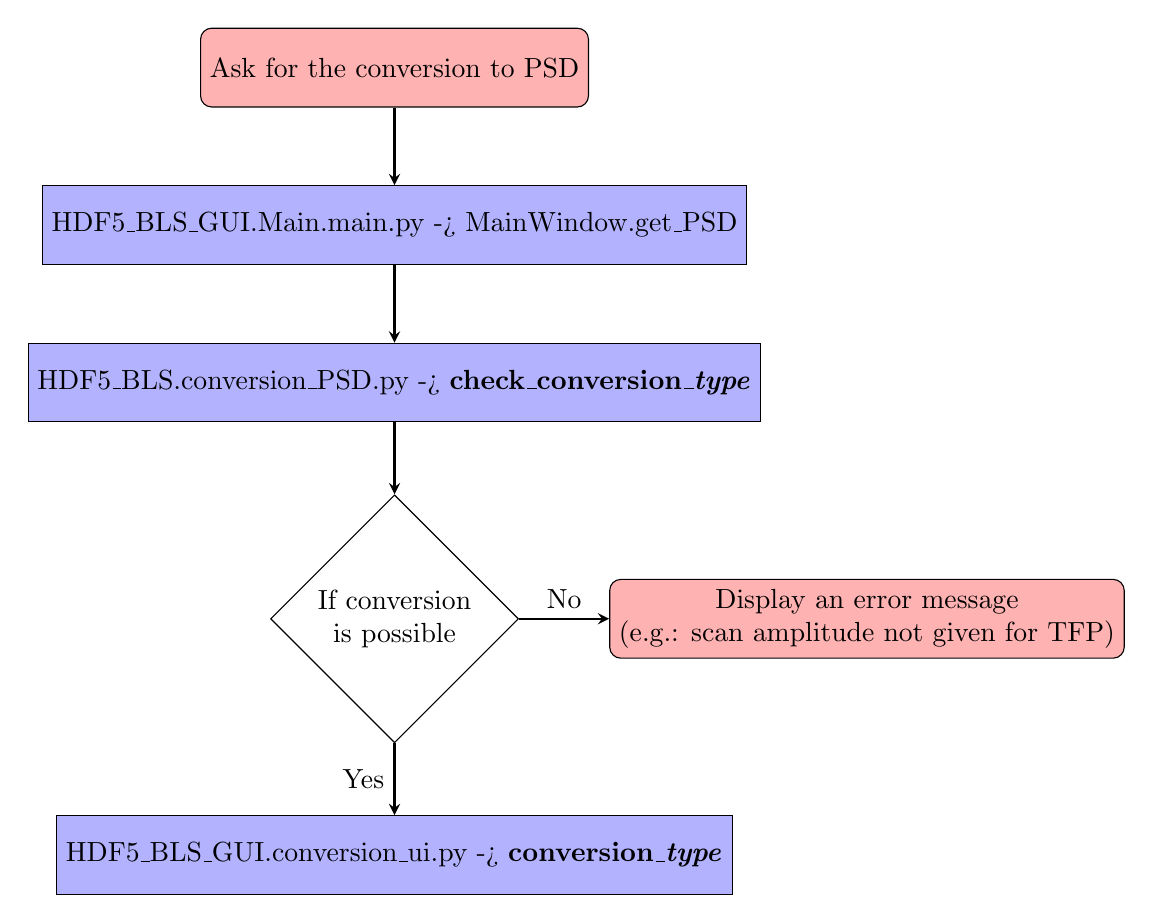
\begin{tikzpicture}[node distance=2cm]

        \node (start) [startstop] {Ask for the conversion to PSD};
        \node (getPSD) [process, below of=start] {HDF5\_BLS\_GUI.Main.main.py -> MainWindow.get\_PSD};
        \node (conversionPSD) [process, below of=getPSD] {HDF5\_BLS.conversion\_PSD.py -> \textbf{check\_conversion\_\textit{type}}};
        \node (if_PSD_possible) [condition, below of=conversionPSD, align = center, yshift=-1cm] {If conversion\\is possible};
        \node (PSD_not_possible) [startstop, right of=if_PSD_possible, align = center, xshift=4cm] {Display an error message\\ (e.g.: scan amplitude not given for TFP)};
        \node (conversionUI) [process, below of=if_PSD_possible, align=center, yshift=-1cm] {HDF5\_BLS\_GUI.conversion\_ui.py -> \textbf{conversion\_\textit{type}}};

        \draw [arrow] (start) -- (getPSD);
        \draw [arrow] (getPSD) -- (conversionPSD);
        \draw [arrow] (conversionPSD) -- (if_PSD_possible);
        \draw [arrow] (if_PSD_possible) -- node[anchor=east] {Yes} (conversionUI);
        \draw [arrow] (if_PSD_possible) -- node[anchor=south] {No} (PSD_not_possible);

    \end{tikzpicture}
\end{center}

To add a routine to convert raw data into a PSD, we'll therefore need to implement the two following functions:
\begin{tcolorbox}
    \paragraph{HDF5\_BLS.conversion\_PSD.check\_conversion\_\textit{type}}
    \begin{itemize}
        \item \textbf{Parameters}:
        \begin{itemize}
            \item wrp: the wrapper associated to the main h5 file. You should always use the parent file as some properties might be inherited.
            \item path: the path to the data we want to treat in the form "Data/Data\_0/..."
        \end{itemize} 
        \item \textbf{Returns}:
        \begin{itemize}
            \item A boolean: True if the conversion is possible, False otherwise. \\
            Depending on the type of spectrometer, the conditions for conversion might be different. In some cases, like for Time Domain experiments, the conversion to PSD will require the user to enter parameters by hand, in other cases, like for TFP, the conversion can only be performed if the scan amplitude is given. The goal of this function is to block any further processing if the conversion is not possible, if the conversion is possible with arguments that are meant to be entered afterwards, it should return True.
        \end{itemize} 
    \end{itemize}
\end{tcolorbox}

Here is an example of the function \texttt{check\_conversion\_ar\_BLS\_VIPA}:
\begin{lstlisting}
def check_conversion_ar_BLS_VIPA(wrapper, path):
    attributes = wrapper.get_attributes_path(path)
    if "TREAT.Center" in attributes.keys():
        return True
    else:
        return False
\end{lstlisting}


\begin{tcolorbox}
    \paragraph{HDF5\_BLS\_GUI.conversion\_ui.conversion\_\textit{type}}:
    \begin{itemize}
        \item \textbf{Parameters}:
        \begin{itemize}
            \item parent: the parent GUI window. This is usefull when you want to open other windows to ask the user for some parameters.
            \item wrp: the wrapper associated to the main h5 file. You should always use the parent file as some properties might be inherited.
            \item path: the path to the data we want to treat in the form "Data/Data\_0/..."
        \end{itemize} 
        \item \textbf{Returns}:
        \begin{itemize}
            \item A dictionnary with the following keys:
            \begin{itemize}
                \item "PSD": the PSD dataset
                \item "Frequency": the frequency dataset
                \item "Process": a text decribing the process of converting the raw data into a PSD. This text is meant to inform the user of the process of converting the data into a PSD.
            \end{itemize}
        \end{itemize} 
    \end{itemize}
\end{tcolorbox}



        \section{Treat data to extract information from a Power Spectral Density} \label{subsec:treatment.toInfo}
            This is a call graph of the functions that are used when asking treat a PSD and frequency. The functions that we will develop have names in bold font. The functions have a fixed nomenclature that we will detail later on, based on the type of spectrometer being used. For this call graph, we will call our spectrometer: \textit{unicorn}:

\begin{center}
    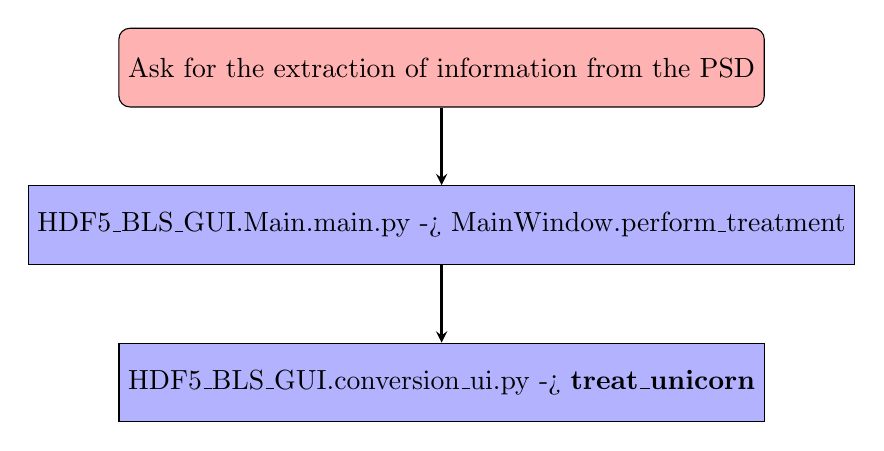
\begin{tikzpicture}[node distance=2cm]

        \node (start) [startstop] {Ask for the extraction of information from the PSD};
        \node (get_treatment) [process, below of=start] {HDF5\_BLS\_GUI.Main.main.py -> MainWindow.perform\_treatment};
        \node (treat_UI) [process, below of=get_treatment, align=center] {HDF5\_BLS\_GUI.conversion\_ui.py -> \textbf{treat\_unicorn}};

        \draw [arrow] (start) -- (get_treatment);
        \draw [arrow] (get_treatment) -- (treat_UI);
    \end{tikzpicture}
\end{center}

To add a routine to extract information from our PSD, we'll therefore need to implement the following functions:

\begin{itemize}
    \item \textit{HDF5\_BLS\_GUI.conversion\_ui.treat\_unicorn}: This function will be used to allow the user to perform a treatment on its data. This function will open a GUI window in the form of a dialog to allow the user to select the parameters of the treatment. Note that this function will not return anything.
\end{itemize}


For GUI compatibility, the function must be called \textit{treat\_type}, where "type" is the type of the spectrometer being used, and placed in the "HDF5\_BLS\_GUI/treat\_ui.py" file. For example if your spectrometer type is "Unicorn", add the following function:
\begin{lstlisting}
def treat_unicorn
\end{lstlisting}

This function must have the following parameters:
    \begin{itemize}
        \item parent: the parent GUI window
        \item wrp: the wrapper associated to the main h5 file
        \item path: the path to the data we want to treat in the form "Data/Data/..."
    \end{itemize}
\begin{lstlisting}
def treat_unicorn(parent, wrp, path):
\end{lstlisting}

From there, there are no guidelines to define your function. The GUI comes however with a few windows that can be inherited from to make the development of custom treatment processes easier. You can find an example of how it was done for the "TFP" treatment in the \hyperref[subsec:example_treatment.TFP]{appendix}.

        \section{Adding a new treatment function} \label{subsec:treatment.new}
            \begin{tcolorbox}
                To do
            \end{tcolorbox}


    \chapter*{Contact}\addcontentsline{toc}{chapter}{Contacts}
        For questions or suggestions, please contact the maintainer at:
        \begin{center}
            \href{mailto:pierre.bouvet@meduniwien.ac.at}{pierre.bouvet@meduniwien.ac.at}.
        \end{center}




\appendix

\part*{Appendix}\addcontentsline{toc}{part}{Appendix}

\chapter{Examples of file structures} \label{chap:examples_file_structures}
    \section{A single measure with no treatment}
        In this first example, we want to store a single measure of a water sample.
    
The following structure represents the base structure of the file:
\begin{verbatim}
    file.h5
    +-- Data (group) -> Name = "Measure"
    |   +-- Data_0 (group) -> Name = "Water"
    |   |   +-- Raw_data (dataset)
\end{verbatim}
Note that we have here added arrows and an example of the value of the "Name" attributes.
    
    \section{A series of measures with no treatment}
        In this second example, we want to store a series of measures taken on three different samples: Water, Ethanol and Glycerol.

The following structure represents the base structure of the file:
\begin{verbatim}
    file.h5
    +-- Data (group) -> Name = "Measure"
    |   +-- Data_0 (group) -> Name = "Water"
    |   |   +-- Raw_data (dataset)
    |   +-- Data_1 (group) -> Name = "Ethanol"
    |   |   +-- Raw_data (dataset)
    |   +-- Data_2 (group) -> Name = "Glycerol"
    |   |   +-- Raw_data (dataset)
\end{verbatim}
Note that we have here added arrows and an example of the value of the "Name" attributes.
    
    \section{A series of series of measures with no treatment but with a calibration spectrum and an impulse response measure}
        In this third example, we want to store a series of two measures taken on two different samples: Water and Ethanol. We also want to store a calibration curve and an impulse response curve.

The following structure represents the base structure of the file:
\begin{verbatim}
    file.h5
    +-- Data (group) -> Name = "Measure"
    |   +-- Data_0 (group) -> Name = "Impulse_Response"
    |   |   +-- Raw_data (dataset)
    |   +-- Data_1 (group) -> Name = "Calibration"
    |   |   +-- Raw_data (dataset)
    |   +-- Data_2 (group) -> Name = "Water"
    |   |   +-- Data_0 (group) -> Name = "Water_01"
    |   |   |   +-- Raw_data (dataset)
    |   |   +-- Data_1 (group) -> Name = "Water_02"
    |   |   |   +-- Raw_data (dataset)
    |   +-- Data_3 (group) -> Name = "Ethanol"
    |   |   +-- Data_0 (group) -> Name = "Ethanol_01"
    |   |   |   +-- Raw_data (dataset)
    |   |   +-- Data_1 (group) -> Name = "Ethanol_02"
    |   |   |   +-- Raw_data (dataset)
\end{verbatim}
Note that we have here added arrows and an example of the value of the "Name" attributes.
    
    \section{A single measure converted to a Power Spectrum Density}
        In this fourth example, we want to store a single measure of a water sample. This measure has been converted into a Power Spectrum Density.

The following structure represents the base structure of the file:
\begin{verbatim}
    file.h5
    +-- Data (group) -> Name = "Measure"
    |   +-- Data_0 (group) -> Name = "Water"
    |   |   +-- Raw_data (dataset)
    |   |   +-- PSD (dataset)
    |   |   +-- Frequency (dataset)
\end{verbatim}
Note that we have here added arrows and an example of the value of the "Name" attributes.
In this case, all the steps of the conversion to PSD are stored in the "Data\_0" group. The nomenclature of the attribute(s) used to store the parameters of the treatment is not specified.
    
    \section{Multiple measures converted to a Power Spectrum Density with a time-independent spectrometer}
        In this fifth example, we are in the situation where a time-independent spectrometer has been used to acquire multiple measures. In this case, the hierrarchy of the file can be used to reduce the number of datasets, by considering that all the PSD share the same frequency axis.

The following structure represents the base structure of the file:
\begin{verbatim}
    file.h5
    +-- Data (group) -> Name = "Measure"
    |   +-- Frequency (dataset)
    |   +-- Data_0 (group) -> Name = "Sample_1"
    |   |   +-- Raw_data (dataset)
    |   |   +-- PSD (dataset)
    |   +-- Data_1 (group) -> Name = "Sample_2"
    |   |   +-- Raw_data (dataset)
    |   |   +-- PSD (dataset)
\end{verbatim}
Note that we have here added arrows and an example of the value of the "Name" attributes.

    \section{A single measure with a treatment}
        In this sixth example, we want to store a single measure of a water sample that has been treated.

The following structure represents the base structure of the file:
\begin{verbatim}
    file.h5
    +-- Data (group) -> Name = "Measure"
    |   +-- Data_0 (group) -> Name = "Water"
    |   |   +-- Raw_data (dataset)
    |   |   +-- PSD (dataset)
    |   |   +-- Frequency (dataset)
    |   |   +-- Treat_0 (group) -> Name = "Treat_5GHz"
    |   |   |   +-- Shift (dataset)
    |   |   |   +-- Shift_err (dataset)
    |   |   |   +-- Linewidth (dataset)
    |   |   |   +-- Linewidth_err (dataset)
\end{verbatim}
Note that we have here added arrows and an example of the value of the "Name" attributes.
In this case, all the steps of the treatment are stored in the "Treat\_0" group. The nomenclature of the attribute(s) used to store the parameters of the treatment is not specified.
    
    \section{A single measure with two distinct treatments}
        In this seventh example, we will store a single measure where two different treatments have been performed (for example a measure at an interface between two materials).

The following structure represents the base structure of the file:
\begin{verbatim}
    file.h5
    +-- Data (group) -> Name = "Measure"
    |   +-- Data_0 (group) -> Name = "Water"
    |   |   +-- Raw_data (dataset)
    |   |   +-- PSD (dataset)
    |   |   +-- Frequency (dataset)
    |   |   +-- Treat_0 (group) -> Name = "Treat_5GHz"
    |   |   |   +-- Shift (dataset)
    |   |   |   +-- Shift_err (dataset)
    |   |   |   +-- Linewidth (dataset)
    |   |   |   +-- Linewidth_err (dataset)
    |   |   +-- Treat_1 (group) -> Name = "Treat_10GHz"
    |   |   |   +-- Shift (dataset)
    |   |   |   +-- Shift_err (dataset)
    |   |   |   +-- Linewidth (dataset)
    |   |   |   +-- Linewidth_err (dataset)
\end{verbatim}
Note that we have here added arrows and an example of the value of the "Name" attributes.
In this case, all the steps of the treatment around 5GHz are stored in the "Treat\_0" group and the ones around 10GHz in the "Treat\_1" group. The nomenclature of the attribute(s) used to store the parameters of the treatment is not specified.

    \section{A single mapping stored as a single measure}
        In this eighth example, we want to store a mapping of a sample. This mapping has been obtained with a spectrometer that returns an array of points for all the points mapped. To clarify this example, we will indicate the dimension of each dataset here between brackets.

The following structure represents the base structure of the file:
\begin{verbatim}
    file.h5
    +-- Data (group) -> Name = "Measure"
    |   +-- Data_0 (group) -> Name = "Sample"
    |   |   +-- Raw_data (dataset) [X, Y, M]
    |   |   +-- PSD (dataset) [X, Y, N]
    |   |   +-- Frequency (dataset) [N]
    |   |   +-- Abscissa_0 (dataset) [X] -> Name = "x (mm)"
    |   |   +-- Abscissa_1 (dataset) [Y] -> Name = "y (mm)"
    |   |   +-- Treat_1 (group) -> Name = "Treat"
    |   |   |   +-- Shift (dataset) [X, Y]
    |   |   |   +-- Shift_std (dataset) [X, Y]
    |   |   |   +-- Linewidth (dataset) [X, Y]
    |   |   |   +-- Linewidth_std (dataset) [X, Y]
\end{verbatim}
Note that we have here added arrows and an example of the value of the "Name" attributes.
    
    \section{A series of mapping over the same field of view stored as a single measure}
        In this ninth example, we are in the situation where multiple mappings of same dimension have been obtained with a spectrometer that returns an array of points for all the points mapped. In this case, the hierrarchy of the file can be used to reduce the number of datasets, by considering that all the PSD share the same frequency axis and the same field of view.

The following structure represents the base structure of the file:
\begin{verbatim}
    file.h5
    +-- Data (group) -> Name = "Measure"
    |   +-- Abscissa_0 (dataset) [X] -> Name = "x (mm)"
    |   +-- Abscissa_1 (dataset) [Y] -> Name = "y (mm)"
    |   +-- Frequency (dataset) [N]
    |   +-- Data_0 (group) -> Name = "Day_1"
    |   |   +-- Raw_data (dataset) [X, Y, M]
    |   |   +-- PSD (dataset) [X, Y, N]
    |   |   +-- Treat_1 (group) -> Name = "Treat"
    |   |   |   +-- Shift (dataset) [X, Y]
    |   |   |   +-- Shift_std (dataset) [X, Y]
    |   |   |   +-- Linewidth (dataset) [X, Y]
    |   |   |   +-- Linewidth_std (dataset) [X, Y]
    |   +-- Data_1 (group) -> Name = "Day_2"
    |   |   +-- Raw_data (dataset) [X, Y, M]
    |   |   +-- PSD (dataset) [X, Y, N]
    |   |   +-- Treat_1 (group) -> Name = "Treat"
    |   |   |   +-- Shift (dataset) [X, Y]
    |   |   |   +-- Shift_std (dataset) [X, Y]
    |   |   |   +-- Linewidth (dataset) [X, Y]
    |   |   |   +-- Linewidth_std (dataset) [X, Y]
\end{verbatim}
Note that we have here added arrows and an example of the value of the "Name" attributes.
    
    \section{A series of mapping over the same field of view stored as multiple measures}
        In this tenth example, we are in the situation where multiple mappings of same dimension have been obtained with a spectrometer that can't return an array of points for all the points mapped, but returns them one by one. Because it would be impractical to create groups for each point, we encourage users to compile their data into a single dataset, and refer to example 9.
    
    \section{A series of mapping obtained with different spectrometers and with different field of view}
        In this eleventh example, we are in the situation where multiple mappings of different dimensions have been obtained with different spectrometers that all return an array of points for all the points mapped. In this case, the hierrarchy of the file cannot be used to reduce the number of datasets, and each group will need its own abscissa and frequency datasets.

The following structure represents the base structure of the file:
\begin{verbatim}
    file.h5
    +-- Data (group) -> Name = "Measure"
    |   +-- Data_0 (group) -> Name = "VIPA"
    |   |   +-- Raw_data (dataset) [X, Y, M]
    |   |   +-- PSD (dataset) [X, Y, N]
    |   |   +-- Abscissa_0 (dataset) [X] -> Name = "x (mm)"
    |   |   +-- Abscissa_1 (dataset) [Y] -> Name = "y (mm)"
    |   |   +-- Frequency (dataset) [N]
    |   |   +-- Treat_1 (group) -> Name = "Treat"
    |   |   |   +-- Shift (dataset) [X, Y]
    |   |   |   +-- Shift_std (dataset) [X, Y]
    |   |   |   +-- Linewidth (dataset) [X, Y]
    |   |   |   +-- Linewidth_std (dataset) [X, Y]
    |   +-- Data_1 (group) -> Name = "TFP"
    |   |   +-- Raw_data (dataset) [X, Y, M]
    |   |   +-- PSD (dataset) [X, Y, N]
    |   |   +-- Abscissa_0 (dataset) [X] -> Name = "x (mm)"
    |   |   +-- Abscissa_1 (dataset) [Y] -> Name = "y (mm)"
    |   |   +-- Frequency (dataset) [N]
    |   |   +-- Treat_1 (group) -> Name = "Treat"
    |   |   |   +-- Shift (dataset) [X, Y]
    |   |   |   +-- Shift_std (dataset) [X, Y]
    |   |   |   +-- Linewidth (dataset) [X, Y]
    |   |   |   +-- Linewidth_std (dataset) [X, Y]
\end{verbatim}
Note that we have here added arrows and an example of the value of the "Name" attributes.

\chapter{Examples of treatment pipelines}
    \section{Treatment of a TFP spectrometer} \label{subsec:example_treatment.TFP}
        \begin{tcolorbox}
    We here present the code that was used to treat the data obtained from a TFP spectrometer. This code is meant to be used as an example of how to write a treatment function for the GUI compatibility. 
\end{tcolorbox}

\begin{enumerate}
    \item We first extract all the PSDs and frequency arrays that are child of the element that has been selected. To do that, we need to go through all the higher layers of our wrapper until our data is found. This is done using the following code:
\begin{lstlisting}
def get_paths_childs(wrp, path = "", frequency = None):
child, freq = [], []
if "Frequency" in wrp.data.keys():
frequency = path+"/Frequency"
for e in wrp.data.keys():
if isinstance(wrp.data[e], wrapper.Wrapper):
    ce, fe = get_paths_childs(wrp.data[e], path+"/"+e, frequency=frequency)
    child += ce
    freq += fe
else:
    if e == "Power Spectral Density":
        freq.append(frequency)
        child.append(path+"/"+e)
return child, freq

# Get the selected data wrapper and frequency array
wrp_temp = wrp
path_loc = path.split("/")[1:]
if "Frequency" in wrp.data.keys(): frequency = wrp.data["Frequency"]
else: frequency = None
for e in path_loc: 
if "Frequency" in wrp_temp.data[e].data.keys(): 
frequency = wrp_temp.data[e].data["Frequency"]
if isinstance(wrp_temp.data[e], wrapper.Wrapper): 
wrp_temp = wrp_temp.data[e]

childs, frequency = get_paths_childs(wrp_temp, path)
\end{lstlisting}
    \item From there we have a choice to make: either we treat each PSD individually or all at once, from some globally defined parameters. We therefore need to ask the user if he wants to treat all of them with the same parameters or each one individually. This is done using the following code:
\begin{lstlisting}
# Display a dialog box to ask the user if he wants to treat all of them with the same parameters or each one individually
msgBox = qtw.QMessageBox()        
msgBox.setText(f"There are {len(childs)} PSD in the selected data. Do you want to treat all of them at once?")
msgBox.setStandardButtons(qtw.QMessageBox.Yes | qtw.QMessageBox.No | qtw.QMessageBox.Cancel)
msgBox.setDefaultButton(qtw.QMessageBox.Yes)
ret = msgBox.exec()
if ret == qtw.QMessageBox.Yes: 
# Treat all PSD at once
elif ret == qtw.QMessageBox.No:
# Treat each PSD individually
\end{lstlisting}
    \item In both cases, we will want to open a window to enter the parameters of the treatment. In the first case, where all the spectra are treated at once, we open the window with all the spectra as parameters. In the second case, where each spectrum is treated individually, we will have a "for" loop to open the window for each spectrum. This is done using the following code:
\begin{lstlisting}
from ParameterCurve.main import TFP_treat

if ret == qtw.QMessageBox.Yes: 
dialog = TFP_treat(parent = parent, wrp_base = wrp, path_base = path, path_curves = childs, path_frequency = frequency)
if dialog.exec_() == qtw.QDialog.Accepted:
# Store all the treated values
elif ret == qtw.QMessageBox.No:
for c,f in zip(childs, frequency):
dialog = TFP_treat(parent = parent, wrp_base = wrp, path_base = path, path_curves = childs, path_frequency = frequency)
if dialog.exec_() == qtw.QDialog.Accepted:
    # Store the treated values
\end{lstlisting}
    Note that here we are importing another GUI window from the \texttt{ParameterCurve} package. The definition of this GUI window is therefore the next step. Let's now look into this \texttt{TFP\_treat} class.
    \item Opening the "HDF5\_BLS\_GUI/ParameterCurve/main.py" file, we define the \texttt{TFP\_treat} class as a daughter of the \texttt{ParameterCurve} class, which is a GUI window with 4 distinct elements:
    \begin{itemize}
        \item A combobox to select the curves to plot at the top left of the window.
        \item A combobox to select the function to apply at the top right of the window.
        \item A graph frame to display the curves at the bottom left of the window.
        \item A frame to display the parameters of the treatment at the bottom right of the window, together with buttons to apply the treatment and to close the window.
    \end{itemize}
\begin{lstlisting}
class TFP_treat(ParameterCurve):
def __init__(self, parent=None, wrp_base = None, path_base = None, path_curves = None, path_frequency = None):
super().__init__(parent, wrp_base.get_child(path_base))
\end{lstlisting}
    This initializes the \texttt{ParameterCurve} class with the wrapper corresponding to all the curves we are going to treat. Giving the class the path of the selected curves displays them by default in the combobox.
    Here is an image of a raw ParameterCurve window after this simple initialization:
    \begin{center}
        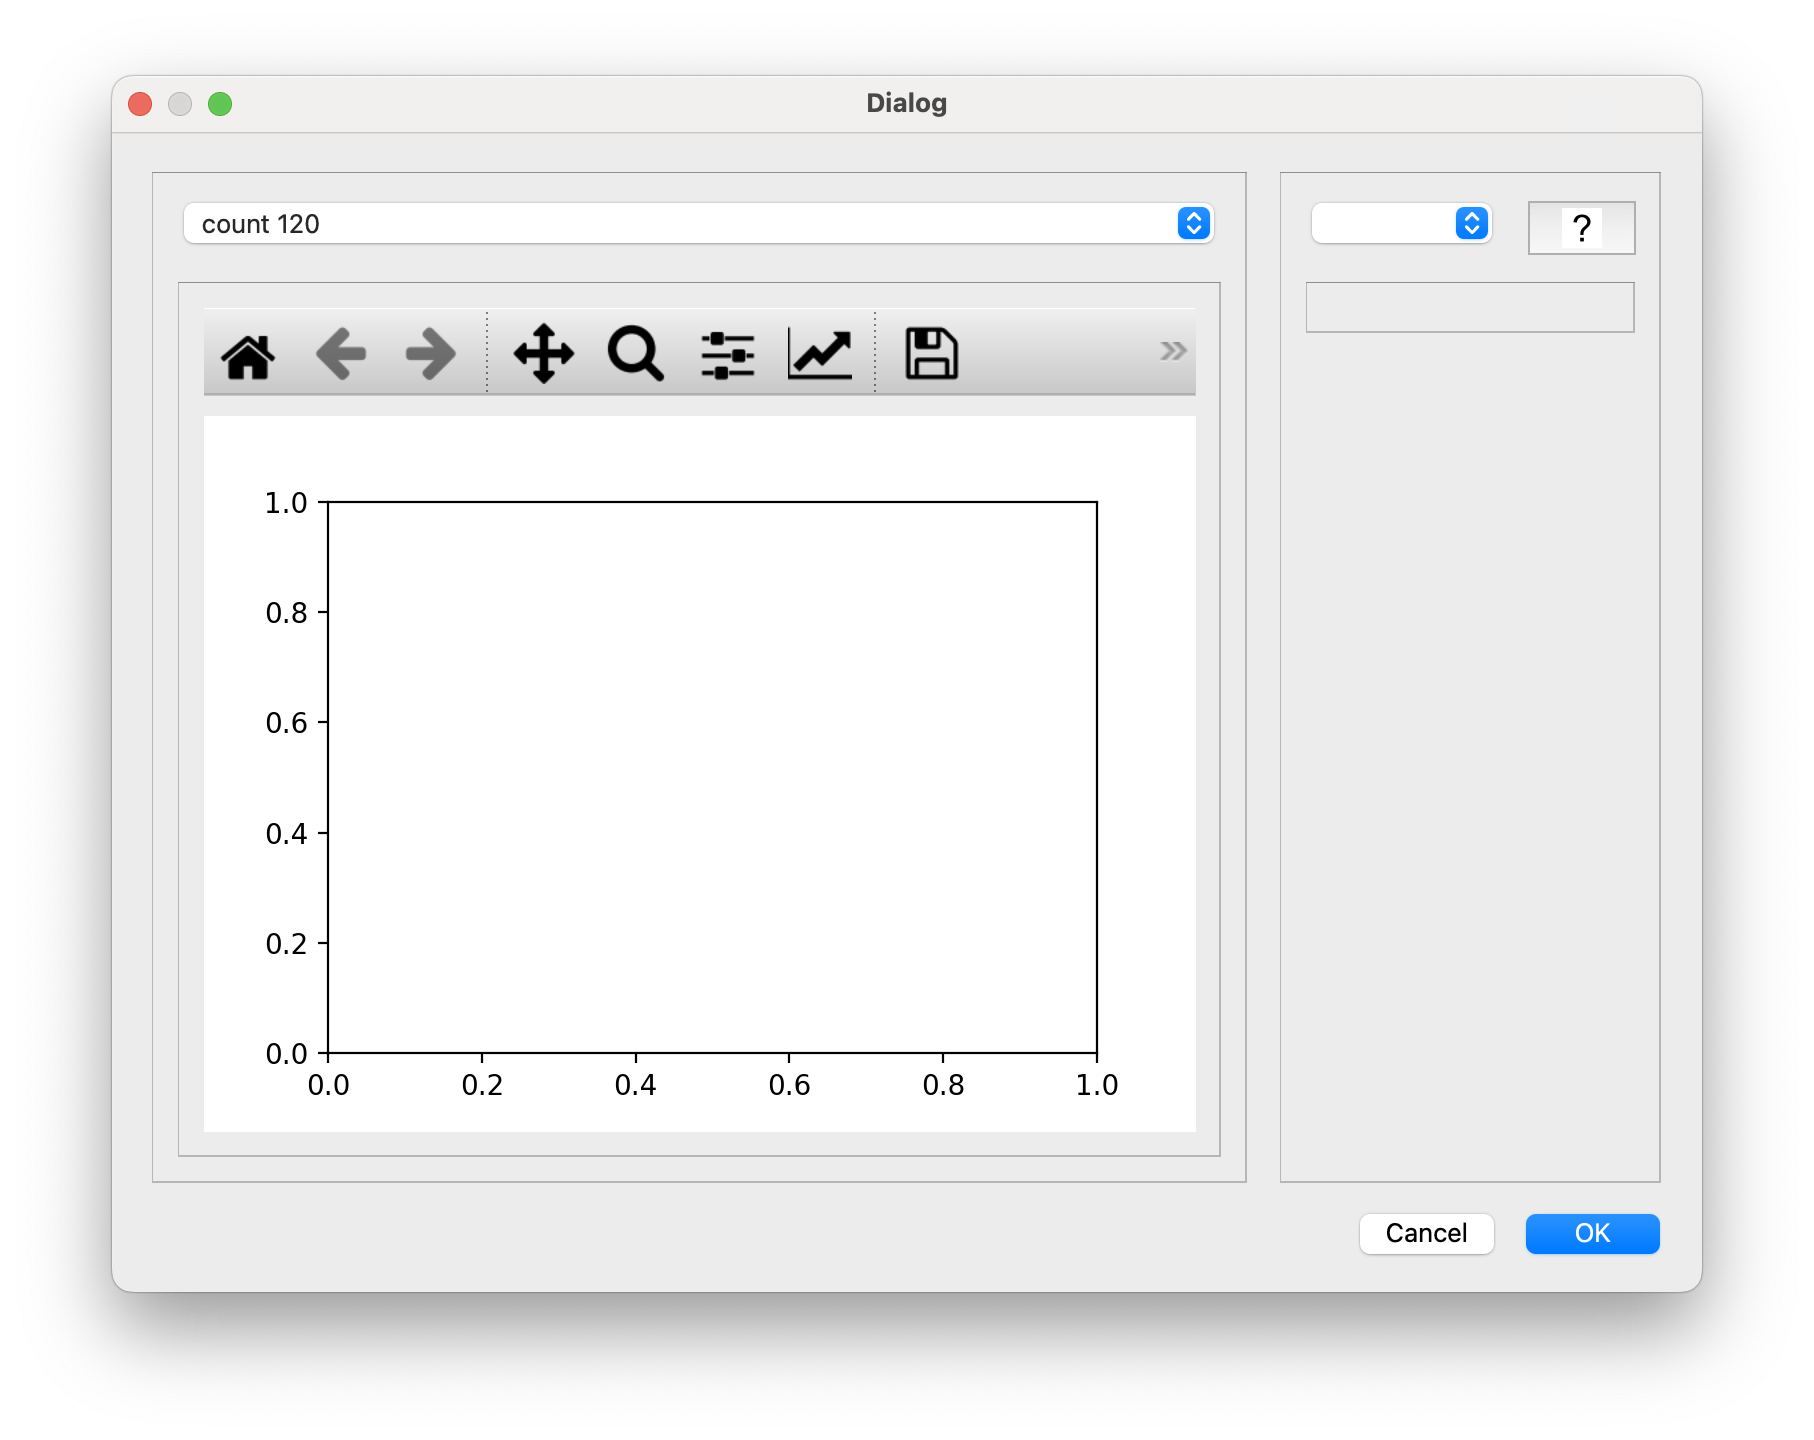
\includegraphics[width=0.9\textwidth]{img/ParameterCurve.png}
    \end{center}
    \item We can now add functionailities to the GUI. First, we display the curve that we select in the combobobx. To do so, we will call the \texttt{handle\_data} function when the combobox is changed. This function will extract the data from the wrapper corresponding to the selected curve and plot it on the graph.
\begin{lstlisting}
def __init__(self, parent=None, wrp_base = None, path_base = None, path_curves = None, path_frequency = None, frequency = None):
super().__init__(parent, wrp_base.get_child(path_base))

if frequency is None:
self.path_curves = path_curves
self.path_frequency = path_frequency
self.path_frequency_unique = None
else:
self.path_curves = None
self.path_frequency = None
self.path_frequency_unique = frequency

# Initializes the graph
self.cb_curves.currentIndexChanged.connect(self.handle_data)
\end{lstlisting}
    Note that we have also stored the paths to the frequencies associated to the curves in respectively the \texttt{path\_frequency} and \texttt{path\_curves} attributes. In the case where only one array is shown, then the path to the frequency array is stored in the \texttt{path\_frequency\_unique} attribute. 
    \item The \texttt{handle\_data} function extracts the path associated to a value in the combobox and gets both the Power Spectral Density and the frequency array from the wrapper corresponding to the selected curve. It then plots the data on the graph.
\begin{lstlisting}
def handle_data(self):
"""
Plots the curve that is currently selected in the combobox. This function also defines self.data and updates the parameters.
"""
# Extract the raw data from the wrapper corresponding to the selected curve in the combobox
wrp = self.wrapper

if len(self.combobox_curve_codes) > 1:
path = self.combobox_curve_codes[self.combobox_curve_names.index(self.cb_curves.currentText())]
path = path[5:]

if type(path) == list:
    for e in path:
        wrp = wrp.data[e]
else:
    wrp = wrp.data[path]

self.data = wrp.data["Power Spectral Density"]
if self.path_frequency is None:
    self.frequency = wrp.get_child(self.path_frequency_unique)[:]
else:
    self.frequency = wrp.get_child(self.path_frequency[self.path_curves.index(path+"/Power Spectral Density")])[:]

# Plot the data
self.graph_canvas.axes.cla()

self.graph_canvas.axes.plot(self.frequency, self.data)
self.graph_canvas.axes.set_xlabel("Frequency Shift (GHz)")
self.graph_canvas.axes.set_ylabel("Intensity (AU)")
self.graph_canvas.draw()
self.update_parameters()
\end{lstlisting}
    Note that the last line of this function is calling the function \texttt{update\_parameters}. This function will update the list of parameters needed to run the treatment. 
    \item We can define the \texttt{update\_parameters} function. This function will most likely be common to most treatments. Its goal is to inspect the "treat" module from the \texttt{HDF5\_BLS} package and extract the list of functions and parameters that are needed automatically. Then it displays the list of functions in the dedicated combobox and the list of parameters in the dedicated frame. If the nomenclature of the parameters and the definition of the treatment function follow a fixed nomenclature, this function automatically links the graph with the relevant parameters so that the graph becomes interactive. Further information about how to develop new treatment functions can be found in section \hyperref[subsec:treatment.new]{Adding a new treatment function}. Out of curiosity, here is the detail of the code of this function:
\begin{lstlisting}
def update_parameters(self):
def initialize_parameters(self, module):
functions = [func for func in getmembers(module, isfunction)]
function_names = [func[0] for func in functions]
functions = [func[1] for func in functions]

self.cb_functions.clear()
self.cb_functions.addItems(function_names)
self.cb_functions.setCurrentIndex(0)
self.cb_functions.currentIndexChanged.connect(lambda: self.show_parameters_function(functions, function_names))

return functions, function_names

def setup_button_help_function(self, functions, function_names):
def show_help_function():
    docstring = functions[function_names.index(self.function_name)].__doc__ or ""
    msgBox = HelpFunction(self, self.function_name, docstring)
    msgBox.exec_()

self.b_helpFunction.clicked.connect(show_help_function)

def onclick_x0(event = None):
if event.inaxes:
    x = float(event.xdata) * 1e6//1
    x = x/1e6
    self.parameters["center_frequency"]["line_edit"].setText(str(x))

def onclick_linewidth(event = None):
if event.inaxes:
    self.temp_linewidth = float(event.xdata)
    self.graph_canvas.mpl_connect('motion_notify_event', on_drag)

def on_drag(event):
if event.inaxes and event.button == 1:
    x1 = float(event.xdata)
linewidth = abs(x1 - self.temp_linewidth) * 1e6//1
linewidth = linewidth/1e6
self.parameters["linewidth"]["line_edit"].setText(str(linewidth))

# Define the module to be used 
import HDF5_BLS.treat as module 

# Extracts the functions and the function names from the module
self.functions, self.function_names = initialize_parameters(self, module)

# Sets the combobox with the functions
self.show_parameters_function(self.functions, self.function_names)

# Adds the models in the dedicated combobox.
Models = module.Models()
self.parameters["c_model"]["combobox"].addItems(Models.models.keys())

# Connects the QLineEdit widget to the onclick_x0 function
self.parameters["center_frequency"]["line_edit"].mousePressEvent = lambda event: self.graph_canvas.mpl_connect('button_press_event', onclick_x0)

# Connects the QLineEdit widget to the onclick_linewidth function
self.parameters["linewidth"]["line_edit"].mousePressEvent = lambda event: self.graph_canvas.mpl_connect('button_press_event', onclick_linewidth)

# Sets the help button to display the function's docstring
setup_button_help_function(self, self.functions, self.function_names)
\end{lstlisting}
    Note that the last line of this function is calling the function \texttt{button\_help\_function}. This function is meant to display the docstring of the function in a dedicated window when the "Help" button is pressed on the interface.
    \item The next step is to allow the user to apply the selected function with the parameters defined in the dedicated frame. To do so, we will setup a "Treat" button in the "setup\_apply\_button" function. 
\begin{lstlisting}
def setup_button_apply(self):
"""
Creates the layout for the buttons to apply the function.
"""
layout = qtw.QGridLayout(self.frame_confirmParam)

button_treat = qtw.QPushButton()
button_treat.setText("Treat")
button_treat.clicked.connect(self.apply_function)

layout.addWidget(button_treat, 0, 0, 1, 1)
\end{lstlisting}
    Note that the button is connected to the \texttt{apply\_function} function. This function returns the entered parameters of the treatement so that it can be performed.
    \item The \texttt{apply\_function} function is meant to read the parameters of the treatment and return an object that will allow the treatment on either one or multiple arrays. This function is developped as a switch between the different treatment functions that were defined in the dedicated combobox. Therefore its structure is the following:
\begin{lstlisting}
def apply_function(self):
"""
Creates the layout for the buttons to apply the function.
"""
func = self.functions[self.function_names.index(self.function_name)]

if self.function_name == "unicorn":
# Extract the parameters proper to the "unicorn" treatment
elif self.function_name == "elf":
# Extract the parameters proper to the "elf" treatment
\end{lstlisting}
    As a more concrete example, here is the code for the \texttt{fit\_model\_v0} treatment function:
\begin{lstlisting}
def apply_function(self):
"""
Extracts the parameters from the GUI and pplies the treatment to the data.
"""
func = self.functions[self.function_names.index(self.function_name)]

if self.function_name == "fit_model_v0":
# Extract the parameters of the function
dic = {}
try:
    dic["center_frequency"] = float(self.parameters["center_frequency"]["line_edit"].text())
    dic["linewidth"] = float(self.parameters["linewidth"]["line_edit"].text())
    dic["normalize"] = not bool(self.parameters["normalize"]["checkbox"].text())
    dic["c_model"] = str(self.parameters["c_model"]["combobox"].currentText())
    dic["fit_S_and_AS"] = not bool(self.parameters["fit_S_and_AS"]["checkbox"].checkState())
    dic["window_peak_find"] = float(self.parameters["window_peak_find"]["line_edit"].text()) 
    dic["window_peak_fit"] = float(self.parameters["window_peak_fit"]["line_edit"].text())
    dic["correct_elastic"] = not bool(self.parameters["correct_elastic"]["checkbox"].checkState())
    IR_wndw = self.parameters["IR_wndw"]["line_edit"].text()
    if IR_wndw == "None": 
        dic["IR_wndw"] = None
    else:
        dic["IR_wndw"] = IR_wndw.replace("(","").replace(")","").replace(" ","")
        dic["IR_wndw"] = tuple(map(float, dic["IR_wndw"].split(",")))

    self.parameter_return["Parameters"] = dic
    self.parameter_return["Function"] = func

    qtw.QMessageBox.information(self, "Treatment parameters stored", "The parameters for the treatment have been stored. You can now close the window to apply the treatment.")

except:
    qtw.QMessageBox.warning(self, "Error while retrieving parameters", "An error happened while retrieving the parameters")
\end{lstlisting}
    Note that the parameters are stored in the "parameter\_return" dictionary. This dictionary is meant to be returned to the \texttt{treat\_ui} module, which will then apply the treatment to the data.
\end{enumerate}
        

\chapter{Specification sheet of the project}
    \renewcommand{\arraystretch}{1.4} % Adjust row height for better readability

\begin{tabular}{|p{1cm}|p{14cm}|}
    \hline
    \rowcolor{grayheavy} 1 & Format \\ \hline

    \rowcolor{graylight} 1.1 & Simplicity \\ \hline

    \rowcolor{graysuperlight} 1.1.1 &  The format should be conceptually simple, unambiguous and easy to create and use. \\ \hline
    \textit{1.1.1.1} & \textit{Storing a single measure should be easy and unambiguous.} \\ \hline
    \textit{1.1.1.2} & \textit{Storing arguments associated with a measure should be easy and unambiguous. The arguments should have a predefined nomenclature.} \\ \hline
    \textit{1.1.1.3} & \textit{Storing measures performed with changes of different hyper parameters should be easy and unambiguous.} \\ \hline
    \textit{1.1.1.4} & \textit{Storing a PSD and Frequency arrays extracted from a measure should be easy and unambiguous.} \\ \hline
    \textit{1.1.1.5} & \textit{Storing the result of a treatment should be easy and unambiguous.} \\ \hline

    \rowcolor{graylight} 1.2 & Universality \\ \hline

    \rowcolor{graysuperlight} 1.2.1 &  The format should be compatible with existing HDF5 softwares. \\ \hline
    \textit{1.2.1.1} & \textit{Opening the file with an HDF5 viewer should give us access to a user-friendly hierarchical structure.} \\ \hline

    \rowcolor{graysuperlight} 1.2.2 &  The format should allow the storage of complemetary datasets obtained with other modalities (e.g. Raman, NMR, fluorescence, etc.). \\ \hline
    \textit{1.2.2.1} & \textit{The format should make a clear distinction between datasets related to BLS measurements and other datasets.} \\ \hline
    \textit{1.2.2.2} & \textit{The format should allow user to store datasets related to other modalities with an arbitrary structure in the first description of the format.} \\ \hline

    \rowcolor{graysuperlight} 1.2.3 &  The format should be adapted for storing Brillouin spectra obtained with different techniques. \\ \hline
    \textit{1.2.3.1} & \textit{The format should allow measures obtained with all techniques to be stored. This includes the sotrage of datasets with arbitrary dimensions, additional technique-specific datasets and additional technique-specific attributes.} \\ \hline

    \rowcolor{graylight} 1.3 & Expandability \\ \hline

    \rowcolor{graysuperlight} 1.3.1 &  The format should accomodate future needs \\ \hline
    \textit{1.3.1.1} & \textit{The format should classify the data preferably by the hyper parameters that were varied for the experiment.} \\ \hline


    \rowcolor{grayheavy} 2 & Analysis and treatment \\ \hline

    \rowcolor{graylight} 2.1 & Power Spectral Density \\ \hline
\end{tabular}

\begin{tabular}{|p{1cm}|p{14cm}|}
    \hline
    \rowcolor{graysuperlight} 2.1.1 &  It must be possible to obtain a Power Spectral Density. \\ \hline
    \textit{2.1.1.1} & \textit{All relevant information and datasets for the obtention of the PSD should be in the same file at the moment of treatment.} \\ \hline
    \textit{2.1.1.2} & \textit{All relevant information and datasets should be unambiguously and simply accessible.} \\ \hline
    \textit{2.1.1.3} & \textit{The PSD and Frequency arrays should be stored unambiguously in the file so that we know which arrays and parameters were used to obtain them.} \\ \hline
    \textit{2.1.1.4} & \textit{The process of obtaining the PSD should be documented in the file in a reusable way.} \\ \hline
    \rowcolor{graysuperlight} 2.1.2 &  It must be possible to create custom algorithms to extract the PSD and frequency. \\ \hline
    \textit{2.1.2.1} & \textit{The function(s) extracting the PSD and frequency should have a fixed nomenclature for their name.} \\ \hline
    \textit{2.1.2.2} & \textit{The function(s) extracting the PSD and frequency should all return the same type of data.} \\ \hline
    \textit{2.1.2.3} & \textit{The function(s) extracting the PSD and frequency should all use the same type of documentation.} \\ \hline
    \textit{2.1.2.4} & \textit{All function(s) extracting the PSD and frequency should be stored in the same module.} \\ \hline
    \textit{2.1.2.5} & \textit{All function(s) extracting the PSD and frequency should also return the parameters they used to obtain the PSD and frequency, with which it is possible to reproduce the PSD and frequency.} \\ \hline

    \rowcolor{graylight} 2.2 & Extraction of peak information \\ \hline
    \rowcolor{graysuperlight}\textit{2.2.1} & \textit{The PSD and Frequency datasets should allow for a unified way of extracting information, independent on the spectrometer used.} \\ \hline
    \textit{2.2.1.1} & \textit{It should be unambiguous to assign a frequency axis to a PSD dataset based on the PSD and Frequency arrays.} \\ \hline

    \rowcolor{graysuperlight}\textit{2.2.2} & \textit{The format should allow the user to extract information with different treatment and store all the results in the same file.} \\ \hline
    \textit{2.2.2.1} & \textit{The treatments should have an identifier that can be incremented to allow the user to store different treatments.} \\ \hline
    \textit{2.2.2.2} & \textit{Each new treatment should also store the parameters used to obtain the information in a way that the user can reproduce the information.} \\ \hline

    \rowcolor{grayheavy} 3 & Graphical User Interface \\ \hline

    \rowcolor{graylight} 3.1 &  Simplicity \\ \hline
    \rowcolor{graysuperlight} 3.1.1 &  Interaction with files and attributes should be as intuitive as possible. \\ \hline
    \textit{3.1.1.1} &  \textit{Adding a file (attribute file or data file) to the format should be possible by dragging and dropping it in the GUI.} \\ \hline
    \textit{3.1.1.2} &  \textit{Changing a visible property of a dataset or group should be possible by left clicking on it and editing its value in the GUI.} \\ \hline
    \textit{3.1.1.3} &  \textit{A right click on a file or group should open a context menu with the action options to perform on the file or group.} \\ \hline
    \textit{3.1.1.4} &  \textit{It should be possible to perform the same action in the GUI by at least 2 redundant ways.}\\ \hline
    \textit{3.1.1.5} &  \textit{The GUI should be idiot proof and be able to flag all actions that might damage the file, make a treatment impossible, or induce any type of incompatibility.}\\ \hline
    


\end{tabular}





\end{document}